\documentclass[twoside]{book}

% Packages required by doxygen
\usepackage{fixltx2e}
\usepackage{calc}
\usepackage{doxygen}
\usepackage[export]{adjustbox} % also loads graphicx
\usepackage{graphicx}
\usepackage[utf8]{inputenc}
\usepackage{makeidx}
\usepackage{multicol}
\usepackage{multirow}
\PassOptionsToPackage{warn}{textcomp}
\usepackage{textcomp}
\usepackage[nointegrals]{wasysym}
\usepackage[table]{xcolor}

% Font selection
\usepackage[T1]{fontenc}
\usepackage[scaled=.90]{helvet}
\usepackage{courier}
\usepackage{amssymb}
\usepackage{sectsty}
\renewcommand{\familydefault}{\sfdefault}
\allsectionsfont{%
  \fontseries{bc}\selectfont%
  \color{darkgray}%
}
\renewcommand{\DoxyLabelFont}{%
  \fontseries{bc}\selectfont%
  \color{darkgray}%
}
\newcommand{\+}{\discretionary{\mbox{\scriptsize$\hookleftarrow$}}{}{}}

% Page & text layout
\usepackage{geometry}
\geometry{%
  a4paper,%
  top=2.5cm,%
  bottom=2.5cm,%
  left=2.5cm,%
  right=2.5cm%
}
\tolerance=750
\hfuzz=15pt
\hbadness=750
\setlength{\emergencystretch}{15pt}
\setlength{\parindent}{0cm}
\setlength{\parskip}{3ex plus 2ex minus 2ex}
\makeatletter
\renewcommand{\paragraph}{%
  \@startsection{paragraph}{4}{0ex}{-1.0ex}{1.0ex}{%
    \normalfont\normalsize\bfseries\SS@parafont%
  }%
}
\renewcommand{\subparagraph}{%
  \@startsection{subparagraph}{5}{0ex}{-1.0ex}{1.0ex}{%
    \normalfont\normalsize\bfseries\SS@subparafont%
  }%
}
\makeatother

% Headers & footers
\usepackage{fancyhdr}
\pagestyle{fancyplain}
\fancyhead[LE]{\fancyplain{}{\bfseries\thepage}}
\fancyhead[CE]{\fancyplain{}{}}
\fancyhead[RE]{\fancyplain{}{\bfseries\leftmark}}
\fancyhead[LO]{\fancyplain{}{\bfseries\rightmark}}
\fancyhead[CO]{\fancyplain{}{}}
\fancyhead[RO]{\fancyplain{}{\bfseries\thepage}}
\fancyfoot[LE]{\fancyplain{}{}}
\fancyfoot[CE]{\fancyplain{}{}}
\fancyfoot[RE]{\fancyplain{}{\bfseries\scriptsize Generated by Doxygen }}
\fancyfoot[LO]{\fancyplain{}{\bfseries\scriptsize Generated by Doxygen }}
\fancyfoot[CO]{\fancyplain{}{}}
\fancyfoot[RO]{\fancyplain{}{}}
\renewcommand{\footrulewidth}{0.4pt}
\renewcommand{\chaptermark}[1]{%
  \markboth{#1}{}%
}
\renewcommand{\sectionmark}[1]{%
  \markright{\thesection\ #1}%
}

% Indices & bibliography
\usepackage{natbib}
\usepackage[titles]{tocloft}
\setcounter{tocdepth}{3}
\setcounter{secnumdepth}{5}
\makeindex

% Hyperlinks (required, but should be loaded last)
\usepackage{ifpdf}
\ifpdf
  \usepackage[pdftex,pagebackref=true]{hyperref}
\else
  \usepackage[ps2pdf,pagebackref=true]{hyperref}
\fi
\hypersetup{%
  colorlinks=true,%
  linkcolor=blue,%
  citecolor=blue,%
  unicode%
}

% Custom commands
\newcommand{\clearemptydoublepage}{%
  \newpage{\pagestyle{empty}\cleardoublepage}%
}

\usepackage{caption}
\captionsetup{labelsep=space,justification=centering,font={bf},singlelinecheck=off,skip=4pt,position=top}

%===== C O N T E N T S =====

\begin{document}

% Titlepage & ToC
\hypersetup{pageanchor=false,
             bookmarksnumbered=true,
             pdfencoding=unicode
            }
\pagenumbering{alph}
\begin{titlepage}
\vspace*{7cm}
\begin{center}%
{\Large My Project }\\
\vspace*{1cm}
{\large Generated by Doxygen 1.8.12}\\
\end{center}
\end{titlepage}
\clearemptydoublepage
\pagenumbering{roman}
\tableofcontents
\clearemptydoublepage
\pagenumbering{arabic}
\hypersetup{pageanchor=true}

%--- Begin generated contents ---
\chapter{Namespace Index}
\section{Namespace List}
Here is a list of all namespaces with brief descriptions\+:\begin{DoxyCompactList}
\item\contentsline{section}{\hyperlink{namespace_fonts}{Fonts} }{\pageref{namespace_fonts}}{}
\item\contentsline{section}{\hyperlink{namespace_music}{Music} }{\pageref{namespace_music}}{}
\item\contentsline{section}{\hyperlink{namespace_scenes}{Scenes} \\*Holds the name/id of each scene }{\pageref{namespace_scenes}}{}
\item\contentsline{section}{\hyperlink{namespacesf}{sf} \\*Handles all the properties of the in game obstacles and items such as the Gas Clouds and the Health Packs }{\pageref{namespacesf}}{}
\item\contentsline{section}{\hyperlink{namespace_shaders}{Shaders} }{\pageref{namespace_shaders}}{}
\item\contentsline{section}{\hyperlink{namespace_sound_effect}{Sound\+Effect} }{\pageref{namespace_sound_effect}}{}
\item\contentsline{section}{\hyperlink{namespace_textures}{Textures} }{\pageref{namespace_textures}}{}
\end{DoxyCompactList}

\chapter{Hierarchical Index}
\section{Class Hierarchy}
This inheritance list is sorted roughly, but not completely, alphabetically\+:\begin{DoxyCompactList}
\item \contentsline{section}{Animation}{\pageref{class_animation}}{}
\item \contentsline{section}{Application}{\pageref{class_application}}{}
\item \contentsline{section}{Astronaut}{\pageref{class_astronaut}}{}
\item \contentsline{section}{Bullet}{\pageref{class_bullet}}{}
\item \contentsline{section}{Camera}{\pageref{class_camera}}{}
\item \contentsline{section}{Scene\+:\+:Context}{\pageref{struct_scene_1_1_context}}{}
\item Drawable\begin{DoxyCompactList}
\item \contentsline{section}{Animated\+Sprite}{\pageref{class_animated_sprite}}{}
\end{DoxyCompactList}
\item \contentsline{section}{Helper}{\pageref{class_helper}}{}
\item Non\+Copyable\begin{DoxyCompactList}
\item \contentsline{section}{Scene\+Stack}{\pageref{class_scene_stack}}{}
\end{DoxyCompactList}
\item \contentsline{section}{Player}{\pageref{class_player}}{}
\item \contentsline{section}{Resource\+Holder$<$ Resource, Identifier $>$}{\pageref{class_resource_holder}}{}
\item \contentsline{section}{Resource\+Holder$<$ sf\+:\+:Font, Fonts\+:\+:ID $>$}{\pageref{class_resource_holder}}{}
\item \contentsline{section}{Resource\+Holder$<$ sf\+:\+:Shader, Shaders\+:\+:ID $>$}{\pageref{class_resource_holder}}{}
\item \contentsline{section}{Resource\+Holder$<$ sf\+:\+:Sound\+Buffer, Sound\+Effect\+:\+:ID $>$}{\pageref{class_resource_holder}}{}
\item \contentsline{section}{Resource\+Holder$<$ sf\+:\+:Texture, Textures\+:\+:ID $>$}{\pageref{class_resource_holder}}{}
\item \contentsline{section}{Scene}{\pageref{class_scene}}{}
\begin{DoxyCompactList}
\item \contentsline{section}{Game\+Scene}{\pageref{class_game_scene}}{}
\item \contentsline{section}{Pause\+Scene}{\pageref{class_pause_scene}}{}
\item \contentsline{section}{Title\+Scene}{\pageref{class_title_scene}}{}
\end{DoxyCompactList}
\item \contentsline{section}{Sound\+Player}{\pageref{class_sound_player}}{}
\item Transformable\begin{DoxyCompactList}
\item \contentsline{section}{Animated\+Sprite}{\pageref{class_animated_sprite}}{}
\end{DoxyCompactList}
\end{DoxyCompactList}

\chapter{Class Index}
\section{Class List}
Here are the classes, structs, unions and interfaces with brief descriptions\+:\begin{DoxyCompactList}
\item\contentsline{section}{\hyperlink{class_a_i}{AI} }{\pageref{class_a_i}}{}
\item\contentsline{section}{\hyperlink{class_alien}{Alien} }{\pageref{class_alien}}{}
\item\contentsline{section}{\hyperlink{class_animated_sprite}{Animated\+Sprite} }{\pageref{class_animated_sprite}}{}
\item\contentsline{section}{\hyperlink{class_animation}{Animation} }{\pageref{class_animation}}{}
\item\contentsline{section}{\hyperlink{class_application}{Application} }{\pageref{class_application}}{}
\item\contentsline{section}{\hyperlink{class_astronaut}{Astronaut} }{\pageref{class_astronaut}}{}
\item\contentsline{section}{\hyperlink{class_bullet}{Bullet} }{\pageref{class_bullet}}{}
\item\contentsline{section}{\hyperlink{class_bullet_manager}{Bullet\+Manager} }{\pageref{class_bullet_manager}}{}
\item\contentsline{section}{\hyperlink{class_camera}{Camera} }{\pageref{class_camera}}{}
\item\contentsline{section}{\hyperlink{class_collision_manager}{Collision\+Manager} }{\pageref{class_collision_manager}}{}
\item\contentsline{section}{\hyperlink{struct_scene_1_1_context}{Scene\+::\+Context} }{\pageref{struct_scene_1_1_context}}{}
\item\contentsline{section}{\hyperlink{class_gameover_scene}{Gameover\+Scene} }{\pageref{class_gameover_scene}}{}
\item\contentsline{section}{\hyperlink{class_game_scene}{Game\+Scene} }{\pageref{class_game_scene}}{}
\item\contentsline{section}{\hyperlink{class_helper}{Helper} }{\pageref{class_helper}}{}
\item\contentsline{section}{\hyperlink{class_h_u_d}{H\+UD} }{\pageref{class_h_u_d}}{}
\item\contentsline{section}{\hyperlink{class_mutant}{Mutant} }{\pageref{class_mutant}}{}
\item\contentsline{section}{\hyperlink{class_nest}{Nest} }{\pageref{class_nest}}{}
\item\contentsline{section}{\hyperlink{class_obstacle}{Obstacle} }{\pageref{class_obstacle}}{}
\item\contentsline{section}{\hyperlink{class_pause_scene}{Pause\+Scene} }{\pageref{class_pause_scene}}{}
\item\contentsline{section}{\hyperlink{class_player}{Player} }{\pageref{class_player}}{}
\item\contentsline{section}{\hyperlink{class_pvector}{Pvector} }{\pageref{class_pvector}}{}
\item\contentsline{section}{\hyperlink{class_resource_holder}{Resource\+Holder$<$ Resource, Identifier $>$} }{\pageref{class_resource_holder}}{}
\item\contentsline{section}{\hyperlink{class_scene}{Scene} }{\pageref{class_scene}}{}
\item\contentsline{section}{\hyperlink{class_scene_stack}{Scene\+Stack} }{\pageref{class_scene_stack}}{}
\item\contentsline{section}{\hyperlink{class_score}{Score} }{\pageref{class_score}}{}
\item\contentsline{section}{\hyperlink{class_sound_player}{Sound\+Player} }{\pageref{class_sound_player}}{}
\item\contentsline{section}{\hyperlink{class_title_scene}{Title\+Scene} }{\pageref{class_title_scene}}{}
\end{DoxyCompactList}

\chapter{File Index}
\section{File List}
Here is a list of all files with brief descriptions\+:\begin{DoxyCompactList}
\item\contentsline{section}{S\+F\+M\+L Engine/\+S\+F\+M\+L Engine/\hyperlink{_animated_sprite_8cpp}{Animated\+Sprite.\+cpp} }{\pageref{_animated_sprite_8cpp}}{}
\item\contentsline{section}{S\+F\+M\+L Engine/\+S\+F\+M\+L Engine/\hyperlink{_animated_sprite_8h}{Animated\+Sprite.\+h} }{\pageref{_animated_sprite_8h}}{}
\item\contentsline{section}{S\+F\+M\+L Engine/\+S\+F\+M\+L Engine/\hyperlink{_animation_8cpp}{Animation.\+cpp} }{\pageref{_animation_8cpp}}{}
\item\contentsline{section}{S\+F\+M\+L Engine/\+S\+F\+M\+L Engine/\hyperlink{_animation_8h}{Animation.\+h} }{\pageref{_animation_8h}}{}
\item\contentsline{section}{S\+F\+M\+L Engine/\+S\+F\+M\+L Engine/\hyperlink{_application_8cpp}{Application.\+cpp} }{\pageref{_application_8cpp}}{}
\item\contentsline{section}{S\+F\+M\+L Engine/\+S\+F\+M\+L Engine/\hyperlink{_application_8h}{Application.\+h} }{\pageref{_application_8h}}{}
\item\contentsline{section}{S\+F\+M\+L Engine/\+S\+F\+M\+L Engine/\hyperlink{_astronaut_8cpp}{Astronaut.\+cpp} }{\pageref{_astronaut_8cpp}}{}
\item\contentsline{section}{S\+F\+M\+L Engine/\+S\+F\+M\+L Engine/\hyperlink{_astronaut_8h}{Astronaut.\+h} }{\pageref{_astronaut_8h}}{}
\item\contentsline{section}{S\+F\+M\+L Engine/\+S\+F\+M\+L Engine/\hyperlink{_bullet_8cpp}{Bullet.\+cpp} }{\pageref{_bullet_8cpp}}{}
\item\contentsline{section}{S\+F\+M\+L Engine/\+S\+F\+M\+L Engine/\hyperlink{_bullet_8h}{Bullet.\+h} }{\pageref{_bullet_8h}}{}
\item\contentsline{section}{S\+F\+M\+L Engine/\+S\+F\+M\+L Engine/\hyperlink{_camera_8cpp}{Camera.\+cpp} }{\pageref{_camera_8cpp}}{}
\item\contentsline{section}{S\+F\+M\+L Engine/\+S\+F\+M\+L Engine/\hyperlink{_camera_8h}{Camera.\+h} }{\pageref{_camera_8h}}{}
\item\contentsline{section}{S\+F\+M\+L Engine/\+S\+F\+M\+L Engine/\hyperlink{_game_scene_8cpp}{Game\+Scene.\+cpp} }{\pageref{_game_scene_8cpp}}{}
\item\contentsline{section}{S\+F\+M\+L Engine/\+S\+F\+M\+L Engine/\hyperlink{_game_scene_8h}{Game\+Scene.\+h} }{\pageref{_game_scene_8h}}{}
\item\contentsline{section}{S\+F\+M\+L Engine/\+S\+F\+M\+L Engine/\hyperlink{_helper_8cpp}{Helper.\+cpp} }{\pageref{_helper_8cpp}}{}
\item\contentsline{section}{S\+F\+M\+L Engine/\+S\+F\+M\+L Engine/\hyperlink{_helper_8h}{Helper.\+h} }{\pageref{_helper_8h}}{}
\item\contentsline{section}{S\+F\+M\+L Engine/\+S\+F\+M\+L Engine/\hyperlink{_pause_scene_8cpp}{Pause\+Scene.\+cpp} }{\pageref{_pause_scene_8cpp}}{}
\item\contentsline{section}{S\+F\+M\+L Engine/\+S\+F\+M\+L Engine/\hyperlink{_pause_scene_8h}{Pause\+Scene.\+h} }{\pageref{_pause_scene_8h}}{}
\item\contentsline{section}{S\+F\+M\+L Engine/\+S\+F\+M\+L Engine/\hyperlink{_player_8cpp}{Player.\+cpp} }{\pageref{_player_8cpp}}{}
\item\contentsline{section}{S\+F\+M\+L Engine/\+S\+F\+M\+L Engine/\hyperlink{_player_8h}{Player.\+h} }{\pageref{_player_8h}}{}
\item\contentsline{section}{S\+F\+M\+L Engine/\+S\+F\+M\+L Engine/\hyperlink{_resource_holder_8h}{Resource\+Holder.\+h} }{\pageref{_resource_holder_8h}}{}
\item\contentsline{section}{S\+F\+M\+L Engine/\+S\+F\+M\+L Engine/\hyperlink{_resource_holder_8inl}{Resource\+Holder.\+inl} }{\pageref{_resource_holder_8inl}}{}
\item\contentsline{section}{S\+F\+M\+L Engine/\+S\+F\+M\+L Engine/\hyperlink{_resource_identifiers_8h}{Resource\+Identifiers.\+h} }{\pageref{_resource_identifiers_8h}}{}
\item\contentsline{section}{S\+F\+M\+L Engine/\+S\+F\+M\+L Engine/\hyperlink{_scene_8cpp}{Scene.\+cpp} }{\pageref{_scene_8cpp}}{}
\item\contentsline{section}{S\+F\+M\+L Engine/\+S\+F\+M\+L Engine/\hyperlink{_scene_8h}{Scene.\+h} }{\pageref{_scene_8h}}{}
\item\contentsline{section}{S\+F\+M\+L Engine/\+S\+F\+M\+L Engine/\hyperlink{_scene_identifiers_8h}{Scene\+Identifiers.\+h} }{\pageref{_scene_identifiers_8h}}{}
\item\contentsline{section}{S\+F\+M\+L Engine/\+S\+F\+M\+L Engine/\hyperlink{_scene_stack_8cpp}{Scene\+Stack.\+cpp} }{\pageref{_scene_stack_8cpp}}{}
\item\contentsline{section}{S\+F\+M\+L Engine/\+S\+F\+M\+L Engine/\hyperlink{_scene_stack_8h}{Scene\+Stack.\+h} }{\pageref{_scene_stack_8h}}{}
\item\contentsline{section}{S\+F\+M\+L Engine/\+S\+F\+M\+L Engine/\hyperlink{_s_f_m_l_01_engine_8cpp}{S\+F\+M\+L Engine.\+cpp} }{\pageref{_s_f_m_l_01_engine_8cpp}}{}
\item\contentsline{section}{S\+F\+M\+L Engine/\+S\+F\+M\+L Engine/\hyperlink{_sound_player_8cpp}{Sound\+Player.\+cpp} }{\pageref{_sound_player_8cpp}}{}
\item\contentsline{section}{S\+F\+M\+L Engine/\+S\+F\+M\+L Engine/\hyperlink{_sound_player_8h}{Sound\+Player.\+h} }{\pageref{_sound_player_8h}}{}
\item\contentsline{section}{S\+F\+M\+L Engine/\+S\+F\+M\+L Engine/\hyperlink{stdafx_8cpp}{stdafx.\+cpp} }{\pageref{stdafx_8cpp}}{}
\item\contentsline{section}{S\+F\+M\+L Engine/\+S\+F\+M\+L Engine/\hyperlink{stdafx_8h}{stdafx.\+h} }{\pageref{stdafx_8h}}{}
\item\contentsline{section}{S\+F\+M\+L Engine/\+S\+F\+M\+L Engine/\hyperlink{targetver_8h}{targetver.\+h} }{\pageref{targetver_8h}}{}
\item\contentsline{section}{S\+F\+M\+L Engine/\+S\+F\+M\+L Engine/\hyperlink{_title_scene_8cpp}{Title\+Scene.\+cpp} }{\pageref{_title_scene_8cpp}}{}
\item\contentsline{section}{S\+F\+M\+L Engine/\+S\+F\+M\+L Engine/\hyperlink{_title_scene_8h}{Title\+Scene.\+h} }{\pageref{_title_scene_8h}}{}
\end{DoxyCompactList}

\chapter{Namespace Documentation}
\hypertarget{namespace_fonts}{}\section{Fonts Namespace Reference}
\label{namespace_fonts}\index{Fonts@{Fonts}}
\subsection*{Enumerations}
\begin{DoxyCompactItemize}
\item 
enum \hyperlink{namespace_fonts_a240717ec0dc75e98501af734a02c396d}{ID} \{ \hyperlink{namespace_fonts_a240717ec0dc75e98501af734a02c396dab947c11fcf1d458feb7709e9c3733e65}{P\+S2P}
 \}
\end{DoxyCompactItemize}


\subsection{Enumeration Type Documentation}
\hypertarget{namespace_fonts_a240717ec0dc75e98501af734a02c396d}{}\label{namespace_fonts_a240717ec0dc75e98501af734a02c396d} 
\index{Fonts@{Fonts}!ID@{ID}}
\index{ID@{ID}!Fonts@{Fonts}}
\subsubsection{\texorpdfstring{ID}{ID}}
{\footnotesize\ttfamily enum \hyperlink{namespace_fonts_a240717ec0dc75e98501af734a02c396d}{Fonts\+::\+ID}}

\begin{DoxyEnumFields}{Enumerator}
\raisebox{\heightof{T}}[0pt][0pt]{\index{P\+S2P@{P\+S2P}!Fonts@{Fonts}}\index{Fonts@{Fonts}!P\+S2P@{P\+S2P}}}\hypertarget{namespace_fonts_a240717ec0dc75e98501af734a02c396dab947c11fcf1d458feb7709e9c3733e65}{}\label{namespace_fonts_a240717ec0dc75e98501af734a02c396dab947c11fcf1d458feb7709e9c3733e65} 
P\+S2P&\\
\hline

\end{DoxyEnumFields}

\hypertarget{namespace_music}{}\section{Music Namespace Reference}
\label{namespace_music}\index{Music@{Music}}
\subsection*{Enumerations}
\begin{DoxyCompactItemize}
\item 
enum \hyperlink{namespace_music_ad5e0c8c2e2e7bdcbffbb125051531b86}{ID} \{ \hyperlink{namespace_music_ad5e0c8c2e2e7bdcbffbb125051531b86a6bcadfc9c1f05aec18efb26a7bec3bc0}{Menu\+Theme}
 \}
\end{DoxyCompactItemize}


\subsection{Enumeration Type Documentation}
\hypertarget{namespace_music_ad5e0c8c2e2e7bdcbffbb125051531b86}{}\label{namespace_music_ad5e0c8c2e2e7bdcbffbb125051531b86} 
\index{Music@{Music}!ID@{ID}}
\index{ID@{ID}!Music@{Music}}
\subsubsection{\texorpdfstring{ID}{ID}}
{\footnotesize\ttfamily enum \hyperlink{namespace_music_ad5e0c8c2e2e7bdcbffbb125051531b86}{Music\+::\+ID}}

\begin{DoxyEnumFields}{Enumerator}
\raisebox{\heightof{T}}[0pt][0pt]{\index{Menu\+Theme@{Menu\+Theme}!Music@{Music}}\index{Music@{Music}!Menu\+Theme@{Menu\+Theme}}}\hypertarget{namespace_music_ad5e0c8c2e2e7bdcbffbb125051531b86a6bcadfc9c1f05aec18efb26a7bec3bc0}{}\label{namespace_music_ad5e0c8c2e2e7bdcbffbb125051531b86a6bcadfc9c1f05aec18efb26a7bec3bc0} 
Menu\+Theme&\\
\hline

\end{DoxyEnumFields}

\hypertarget{namespace_scenes}{}\section{Scenes Namespace Reference}
\label{namespace_scenes}\index{Scenes@{Scenes}}
\subsection*{Enumerations}
\begin{DoxyCompactItemize}
\item 
enum \hyperlink{namespace_scenes_a0ad7ab6856b1d77d498e3a251f6bb275}{ID} \{ \newline
\hyperlink{namespace_scenes_a0ad7ab6856b1d77d498e3a251f6bb275a62ed6cc2cc350c0b2f007bba07e0aac6}{None}, 
\hyperlink{namespace_scenes_a0ad7ab6856b1d77d498e3a251f6bb275a777d5475dda0030fdd34a9f736b5891a}{Title}, 
\hyperlink{namespace_scenes_a0ad7ab6856b1d77d498e3a251f6bb275a8c6d665468f36f79d9f0b1d02ec46b74}{Menu}, 
\hyperlink{namespace_scenes_a0ad7ab6856b1d77d498e3a251f6bb275a1c09bc977521c21c5bd955eca43c24f1}{Game}, 
\newline
\hyperlink{namespace_scenes_a0ad7ab6856b1d77d498e3a251f6bb275aa64f4adb0e245eb77f79e2cf3c2c10e7}{Loading}, 
\hyperlink{namespace_scenes_a0ad7ab6856b1d77d498e3a251f6bb275a554bcf6b884325cfc3097b9d12f3d97b}{Pause}, 
\hyperlink{namespace_scenes_a0ad7ab6856b1d77d498e3a251f6bb275a81c375e87af8f99a546d728ce60e4620}{Settings}, 
\hyperlink{namespace_scenes_a0ad7ab6856b1d77d498e3a251f6bb275aca2e7abcafce28f8ca6e764360a04047}{Gameover}
 \}
\end{DoxyCompactItemize}


\subsection{Enumeration Type Documentation}
\mbox{\Hypertarget{namespace_scenes_a0ad7ab6856b1d77d498e3a251f6bb275}\label{namespace_scenes_a0ad7ab6856b1d77d498e3a251f6bb275}} 
\index{Scenes@{Scenes}!ID@{ID}}
\index{ID@{ID}!Scenes@{Scenes}}
\subsubsection{\texorpdfstring{ID}{ID}}
{\footnotesize\ttfamily enum \hyperlink{namespace_scenes_a0ad7ab6856b1d77d498e3a251f6bb275}{Scenes\+::\+ID}}

\begin{DoxyEnumFields}{Enumerator}
\raisebox{\heightof{T}}[0pt][0pt]{\index{None@{None}!Scenes@{Scenes}}\index{Scenes@{Scenes}!None@{None}}}\mbox{\Hypertarget{namespace_scenes_a0ad7ab6856b1d77d498e3a251f6bb275a62ed6cc2cc350c0b2f007bba07e0aac6}\label{namespace_scenes_a0ad7ab6856b1d77d498e3a251f6bb275a62ed6cc2cc350c0b2f007bba07e0aac6}} 
None&\\
\hline

\raisebox{\heightof{T}}[0pt][0pt]{\index{Title@{Title}!Scenes@{Scenes}}\index{Scenes@{Scenes}!Title@{Title}}}\mbox{\Hypertarget{namespace_scenes_a0ad7ab6856b1d77d498e3a251f6bb275a777d5475dda0030fdd34a9f736b5891a}\label{namespace_scenes_a0ad7ab6856b1d77d498e3a251f6bb275a777d5475dda0030fdd34a9f736b5891a}} 
Title&\\
\hline

\raisebox{\heightof{T}}[0pt][0pt]{\index{Menu@{Menu}!Scenes@{Scenes}}\index{Scenes@{Scenes}!Menu@{Menu}}}\mbox{\Hypertarget{namespace_scenes_a0ad7ab6856b1d77d498e3a251f6bb275a8c6d665468f36f79d9f0b1d02ec46b74}\label{namespace_scenes_a0ad7ab6856b1d77d498e3a251f6bb275a8c6d665468f36f79d9f0b1d02ec46b74}} 
Menu&\\
\hline

\raisebox{\heightof{T}}[0pt][0pt]{\index{Game@{Game}!Scenes@{Scenes}}\index{Scenes@{Scenes}!Game@{Game}}}\mbox{\Hypertarget{namespace_scenes_a0ad7ab6856b1d77d498e3a251f6bb275a1c09bc977521c21c5bd955eca43c24f1}\label{namespace_scenes_a0ad7ab6856b1d77d498e3a251f6bb275a1c09bc977521c21c5bd955eca43c24f1}} 
Game&\\
\hline

\raisebox{\heightof{T}}[0pt][0pt]{\index{Loading@{Loading}!Scenes@{Scenes}}\index{Scenes@{Scenes}!Loading@{Loading}}}\mbox{\Hypertarget{namespace_scenes_a0ad7ab6856b1d77d498e3a251f6bb275aa64f4adb0e245eb77f79e2cf3c2c10e7}\label{namespace_scenes_a0ad7ab6856b1d77d498e3a251f6bb275aa64f4adb0e245eb77f79e2cf3c2c10e7}} 
Loading&\\
\hline

\raisebox{\heightof{T}}[0pt][0pt]{\index{Pause@{Pause}!Scenes@{Scenes}}\index{Scenes@{Scenes}!Pause@{Pause}}}\mbox{\Hypertarget{namespace_scenes_a0ad7ab6856b1d77d498e3a251f6bb275a554bcf6b884325cfc3097b9d12f3d97b}\label{namespace_scenes_a0ad7ab6856b1d77d498e3a251f6bb275a554bcf6b884325cfc3097b9d12f3d97b}} 
Pause&\\
\hline

\raisebox{\heightof{T}}[0pt][0pt]{\index{Settings@{Settings}!Scenes@{Scenes}}\index{Scenes@{Scenes}!Settings@{Settings}}}\mbox{\Hypertarget{namespace_scenes_a0ad7ab6856b1d77d498e3a251f6bb275a81c375e87af8f99a546d728ce60e4620}\label{namespace_scenes_a0ad7ab6856b1d77d498e3a251f6bb275a81c375e87af8f99a546d728ce60e4620}} 
Settings&\\
\hline

\raisebox{\heightof{T}}[0pt][0pt]{\index{Gameover@{Gameover}!Scenes@{Scenes}}\index{Scenes@{Scenes}!Gameover@{Gameover}}}\mbox{\Hypertarget{namespace_scenes_a0ad7ab6856b1d77d498e3a251f6bb275aca2e7abcafce28f8ca6e764360a04047}\label{namespace_scenes_a0ad7ab6856b1d77d498e3a251f6bb275aca2e7abcafce28f8ca6e764360a04047}} 
Gameover&\\
\hline

\end{DoxyEnumFields}

\hypertarget{namespacesf}{}\section{sf Namespace Reference}
\label{namespacesf}\index{sf@{sf}}


Handles all the properties of the in game obstacles and items such as the Gas Clouds and the Health Packs.  




\subsection{Detailed Description}
Handles all the properties of the in game obstacles and items such as the Gas Clouds and the Health Packs. 


\hypertarget{namespace_shaders}{}\section{Shaders Namespace Reference}
\label{namespace_shaders}\index{Shaders@{Shaders}}
\subsection*{Enumerations}
\begin{DoxyCompactItemize}
\item 
enum \hyperlink{namespace_shaders_ac69c86b4e324fdda75990b34e9a1dc7e}{ID} \{ \hyperlink{namespace_shaders_ac69c86b4e324fdda75990b34e9a1dc7eaf02a64b9b6206367e82aae811cd52d1b}{Shockwave}, 
\hyperlink{namespace_shaders_ac69c86b4e324fdda75990b34e9a1dc7eaa670629dfa701b0829eec82754034c35}{Ripple}
 \}
\end{DoxyCompactItemize}


\subsection{Enumeration Type Documentation}
\mbox{\Hypertarget{namespace_shaders_ac69c86b4e324fdda75990b34e9a1dc7e}\label{namespace_shaders_ac69c86b4e324fdda75990b34e9a1dc7e}} 
\index{Shaders@{Shaders}!ID@{ID}}
\index{ID@{ID}!Shaders@{Shaders}}
\subsubsection{\texorpdfstring{ID}{ID}}
{\footnotesize\ttfamily enum \hyperlink{namespace_shaders_ac69c86b4e324fdda75990b34e9a1dc7e}{Shaders\+::\+ID}}

\begin{DoxyEnumFields}{Enumerator}
\raisebox{\heightof{T}}[0pt][0pt]{\index{Shockwave@{Shockwave}!Shaders@{Shaders}}\index{Shaders@{Shaders}!Shockwave@{Shockwave}}}\mbox{\Hypertarget{namespace_shaders_ac69c86b4e324fdda75990b34e9a1dc7eaf02a64b9b6206367e82aae811cd52d1b}\label{namespace_shaders_ac69c86b4e324fdda75990b34e9a1dc7eaf02a64b9b6206367e82aae811cd52d1b}} 
Shockwave&\\
\hline

\raisebox{\heightof{T}}[0pt][0pt]{\index{Ripple@{Ripple}!Shaders@{Shaders}}\index{Shaders@{Shaders}!Ripple@{Ripple}}}\mbox{\Hypertarget{namespace_shaders_ac69c86b4e324fdda75990b34e9a1dc7eaa670629dfa701b0829eec82754034c35}\label{namespace_shaders_ac69c86b4e324fdda75990b34e9a1dc7eaa670629dfa701b0829eec82754034c35}} 
Ripple&\\
\hline

\end{DoxyEnumFields}

\hypertarget{namespace_sound_effect}{}\section{Sound\+Effect Namespace Reference}
\label{namespace_sound_effect}\index{Sound\+Effect@{Sound\+Effect}}
\subsection*{Enumerations}
\begin{DoxyCompactItemize}
\item 
enum \hyperlink{namespace_sound_effect_a11ffbf1eb89e85a34cbfd5a59b2cd9cb}{ID} \{ \hyperlink{namespace_sound_effect_a11ffbf1eb89e85a34cbfd5a59b2cd9cba089c46ca5650d2908d73313697639681}{Charge}
 \}
\end{DoxyCompactItemize}


\subsection{Enumeration Type Documentation}
\mbox{\Hypertarget{namespace_sound_effect_a11ffbf1eb89e85a34cbfd5a59b2cd9cb}\label{namespace_sound_effect_a11ffbf1eb89e85a34cbfd5a59b2cd9cb}} 
\index{Sound\+Effect@{Sound\+Effect}!ID@{ID}}
\index{ID@{ID}!Sound\+Effect@{Sound\+Effect}}
\subsubsection{\texorpdfstring{ID}{ID}}
{\footnotesize\ttfamily enum \hyperlink{namespace_sound_effect_a11ffbf1eb89e85a34cbfd5a59b2cd9cb}{Sound\+Effect\+::\+ID}}

\begin{DoxyEnumFields}{Enumerator}
\raisebox{\heightof{T}}[0pt][0pt]{\index{Charge@{Charge}!Sound\+Effect@{Sound\+Effect}}\index{Sound\+Effect@{Sound\+Effect}!Charge@{Charge}}}\mbox{\Hypertarget{namespace_sound_effect_a11ffbf1eb89e85a34cbfd5a59b2cd9cba089c46ca5650d2908d73313697639681}\label{namespace_sound_effect_a11ffbf1eb89e85a34cbfd5a59b2cd9cba089c46ca5650d2908d73313697639681}} 
Charge&\\
\hline

\end{DoxyEnumFields}

\hypertarget{namespace_textures}{}\section{Textures Namespace Reference}
\label{namespace_textures}\index{Textures@{Textures}}
\subsection*{Enumerations}
\begin{DoxyCompactItemize}
\item 
enum \hyperlink{namespace_textures_a2cfe2099537d4e80b08437b4978301a5}{ID} \{ \newline
\hyperlink{namespace_textures_a2cfe2099537d4e80b08437b4978301a5aa7eca1b35d39c70635eb67e8d21dc819}{Playo}, 
\hyperlink{namespace_textures_a2cfe2099537d4e80b08437b4978301a5a61cbf1132258cda586a6130a03e804c9}{Astro}, 
\hyperlink{namespace_textures_a2cfe2099537d4e80b08437b4978301a5ae0de724966274dc241ef3de7eadc396d}{Nest}, 
\hyperlink{namespace_textures_a2cfe2099537d4e80b08437b4978301a5a52aa97e3cdb226168982426b7ab0aa2d}{Game\+Background}, 
\newline
\hyperlink{namespace_textures_a2cfe2099537d4e80b08437b4978301a5aa39a5e3bca9832daaaa9cbf31b8961f9}{Pause\+Background}, 
\hyperlink{namespace_textures_a2cfe2099537d4e80b08437b4978301a5aa7d0eb38e6c55469c163efe01cb88695}{Main\+Menu\+BG}, 
\hyperlink{namespace_textures_a2cfe2099537d4e80b08437b4978301a5a24f167674de87c1108c92fffd3837cd0}{Game\+Over\+BG}, 
\hyperlink{namespace_textures_a2cfe2099537d4e80b08437b4978301a5ac583013e9c40cfacce00147270928966}{Button}, 
\newline
\hyperlink{namespace_textures_a2cfe2099537d4e80b08437b4978301a5a34760cfde35030b2a2e35c8e81d6602a}{H\+UD}, 
\hyperlink{namespace_textures_a2cfe2099537d4e80b08437b4978301a5aa9db10d857958d53d192c3165dead752}{Gas\+Cloud}
 \}
\end{DoxyCompactItemize}


\subsection{Enumeration Type Documentation}
\mbox{\Hypertarget{namespace_textures_a2cfe2099537d4e80b08437b4978301a5}\label{namespace_textures_a2cfe2099537d4e80b08437b4978301a5}} 
\index{Textures@{Textures}!ID@{ID}}
\index{ID@{ID}!Textures@{Textures}}
\subsubsection{\texorpdfstring{ID}{ID}}
{\footnotesize\ttfamily enum \hyperlink{namespace_textures_a2cfe2099537d4e80b08437b4978301a5}{Textures\+::\+ID}}

\begin{DoxyEnumFields}{Enumerator}
\raisebox{\heightof{T}}[0pt][0pt]{\index{Playo@{Playo}!Textures@{Textures}}\index{Textures@{Textures}!Playo@{Playo}}}\mbox{\Hypertarget{namespace_textures_a2cfe2099537d4e80b08437b4978301a5aa7eca1b35d39c70635eb67e8d21dc819}\label{namespace_textures_a2cfe2099537d4e80b08437b4978301a5aa7eca1b35d39c70635eb67e8d21dc819}} 
Playo&\\
\hline

\raisebox{\heightof{T}}[0pt][0pt]{\index{Astro@{Astro}!Textures@{Textures}}\index{Textures@{Textures}!Astro@{Astro}}}\mbox{\Hypertarget{namespace_textures_a2cfe2099537d4e80b08437b4978301a5a61cbf1132258cda586a6130a03e804c9}\label{namespace_textures_a2cfe2099537d4e80b08437b4978301a5a61cbf1132258cda586a6130a03e804c9}} 
Astro&\\
\hline

\raisebox{\heightof{T}}[0pt][0pt]{\index{Nest@{Nest}!Textures@{Textures}}\index{Textures@{Textures}!Nest@{Nest}}}\mbox{\Hypertarget{namespace_textures_a2cfe2099537d4e80b08437b4978301a5ae0de724966274dc241ef3de7eadc396d}\label{namespace_textures_a2cfe2099537d4e80b08437b4978301a5ae0de724966274dc241ef3de7eadc396d}} 
Nest&\\
\hline

\raisebox{\heightof{T}}[0pt][0pt]{\index{Game\+Background@{Game\+Background}!Textures@{Textures}}\index{Textures@{Textures}!Game\+Background@{Game\+Background}}}\mbox{\Hypertarget{namespace_textures_a2cfe2099537d4e80b08437b4978301a5a52aa97e3cdb226168982426b7ab0aa2d}\label{namespace_textures_a2cfe2099537d4e80b08437b4978301a5a52aa97e3cdb226168982426b7ab0aa2d}} 
Game\+Background&\\
\hline

\raisebox{\heightof{T}}[0pt][0pt]{\index{Pause\+Background@{Pause\+Background}!Textures@{Textures}}\index{Textures@{Textures}!Pause\+Background@{Pause\+Background}}}\mbox{\Hypertarget{namespace_textures_a2cfe2099537d4e80b08437b4978301a5aa39a5e3bca9832daaaa9cbf31b8961f9}\label{namespace_textures_a2cfe2099537d4e80b08437b4978301a5aa39a5e3bca9832daaaa9cbf31b8961f9}} 
Pause\+Background&\\
\hline

\raisebox{\heightof{T}}[0pt][0pt]{\index{Main\+Menu\+BG@{Main\+Menu\+BG}!Textures@{Textures}}\index{Textures@{Textures}!Main\+Menu\+BG@{Main\+Menu\+BG}}}\mbox{\Hypertarget{namespace_textures_a2cfe2099537d4e80b08437b4978301a5aa7d0eb38e6c55469c163efe01cb88695}\label{namespace_textures_a2cfe2099537d4e80b08437b4978301a5aa7d0eb38e6c55469c163efe01cb88695}} 
Main\+Menu\+BG&\\
\hline

\raisebox{\heightof{T}}[0pt][0pt]{\index{Game\+Over\+BG@{Game\+Over\+BG}!Textures@{Textures}}\index{Textures@{Textures}!Game\+Over\+BG@{Game\+Over\+BG}}}\mbox{\Hypertarget{namespace_textures_a2cfe2099537d4e80b08437b4978301a5a24f167674de87c1108c92fffd3837cd0}\label{namespace_textures_a2cfe2099537d4e80b08437b4978301a5a24f167674de87c1108c92fffd3837cd0}} 
Game\+Over\+BG&\\
\hline

\raisebox{\heightof{T}}[0pt][0pt]{\index{Button@{Button}!Textures@{Textures}}\index{Textures@{Textures}!Button@{Button}}}\mbox{\Hypertarget{namespace_textures_a2cfe2099537d4e80b08437b4978301a5ac583013e9c40cfacce00147270928966}\label{namespace_textures_a2cfe2099537d4e80b08437b4978301a5ac583013e9c40cfacce00147270928966}} 
Button&\\
\hline

\raisebox{\heightof{T}}[0pt][0pt]{\index{H\+UD@{H\+UD}!Textures@{Textures}}\index{Textures@{Textures}!H\+UD@{H\+UD}}}\mbox{\Hypertarget{namespace_textures_a2cfe2099537d4e80b08437b4978301a5a34760cfde35030b2a2e35c8e81d6602a}\label{namespace_textures_a2cfe2099537d4e80b08437b4978301a5a34760cfde35030b2a2e35c8e81d6602a}} 
H\+UD&\\
\hline

\raisebox{\heightof{T}}[0pt][0pt]{\index{Gas\+Cloud@{Gas\+Cloud}!Textures@{Textures}}\index{Textures@{Textures}!Gas\+Cloud@{Gas\+Cloud}}}\mbox{\Hypertarget{namespace_textures_a2cfe2099537d4e80b08437b4978301a5aa9db10d857958d53d192c3165dead752}\label{namespace_textures_a2cfe2099537d4e80b08437b4978301a5aa9db10d857958d53d192c3165dead752}} 
Gas\+Cloud&\\
\hline

\end{DoxyEnumFields}

\chapter{Class Documentation}
\hypertarget{class_animated_sprite}{}\section{Animated\+Sprite Class Reference}
\label{class_animated_sprite}\index{Animated\+Sprite@{Animated\+Sprite}}


{\ttfamily \#include $<$Animated\+Sprite.\+h$>$}

Inheritance diagram for Animated\+Sprite\+:\begin{figure}[H]
\begin{center}
\leavevmode
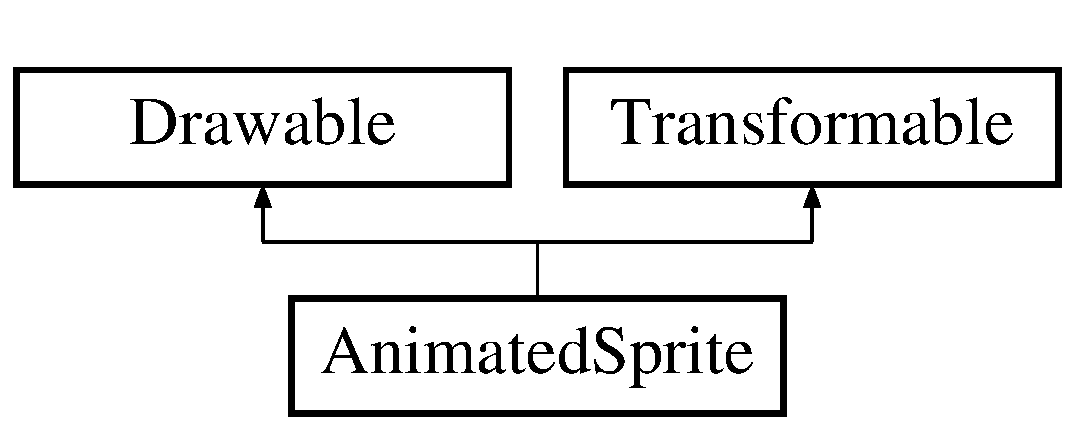
\includegraphics[height=2.000000cm]{class_animated_sprite}
\end{center}
\end{figure}
\subsection*{Public Member Functions}
\begin{DoxyCompactItemize}
\item 
\hyperlink{class_animated_sprite_a097ab8444824e7085d71a1f7144e7763}{Animated\+Sprite} (sf\+::\+Time frame\+Time=sf\+::seconds(0.\+2f), bool paused=false, bool looped=true)
\item 
void \hyperlink{class_animated_sprite_a17a41ff812631a9d8947d272933d6696}{update} (sf\+::\+Time delta\+Time)
\item 
void \hyperlink{class_animated_sprite_ab1afc57d90d57a0c4bc4f5b090f2dacf}{set\+Animation} (const \hyperlink{class_animation}{Animation} \&animation)
\item 
void \hyperlink{class_animated_sprite_af598fab5c3599ccc5ed1e2d4fefa68cc}{set\+Frame\+Time} (sf\+::\+Time time)
\item 
void \hyperlink{class_animated_sprite_a203b968f1cb374cca5dbc89716174020}{play} ()
\item 
void \hyperlink{class_animated_sprite_a9ea345649a4e012d096bc04aafe1ecb0}{play} (const \hyperlink{class_animation}{Animation} \&animation)
\item 
void \hyperlink{class_animated_sprite_a48384db59427423b5c1d98f6ee94fe45}{pause} ()
\item 
void \hyperlink{class_animated_sprite_af9734f4346d3d2370322b2dcaeef133c}{stop} ()
\item 
void \hyperlink{class_animated_sprite_a855a5a48ea2e1c51c7c9304857dd2f8c}{set\+Looped} (bool looped)
\item 
void \hyperlink{class_animated_sprite_a1a96a0f6570efddd2eb26f89bc5b6f50}{set\+Color} (const sf\+::\+Color \&color)
\item 
const \hyperlink{class_animation}{Animation} $\ast$ \hyperlink{class_animated_sprite_a03bacdbaf638cb6f7987e342980206c2}{get\+Animation} () const
\item 
sf\+::\+Float\+Rect \hyperlink{class_animated_sprite_ac4c88435c8698f452629c5cd78bfb3c9}{get\+Local\+Bounds} () const
\item 
sf\+::\+Float\+Rect \hyperlink{class_animated_sprite_a86dca0906c53b3e630aaeac2f0085a0e}{get\+Global\+Bounds} () const
\item 
bool \hyperlink{class_animated_sprite_aaf2c2fb0e1487e689af4a6bbeb7e3e85}{is\+Looped} () const
\item 
bool \hyperlink{class_animated_sprite_a55f450add05d45e5369a6ad24f9e438f}{is\+Playing} () const
\item 
sf\+::\+Time \hyperlink{class_animated_sprite_a5291f8e24fe2c6e4284bc7ff9499ef77}{get\+Frame\+Time} () const
\item 
void \hyperlink{class_animated_sprite_a0b3e38fffdc1d29f46fa08df9ef2a747}{set\+Frame} (std\+::size\+\_\+t new\+Frame, bool reset\+Time=true)
\item 
int \hyperlink{class_animated_sprite_a8e929c48b0ca713b7aac7dd769e4f00c}{get\+Frame} ()
\end{DoxyCompactItemize}


\subsection{Constructor \& Destructor Documentation}
\mbox{\Hypertarget{class_animated_sprite_a097ab8444824e7085d71a1f7144e7763}\label{class_animated_sprite_a097ab8444824e7085d71a1f7144e7763}} 
\index{Animated\+Sprite@{Animated\+Sprite}!Animated\+Sprite@{Animated\+Sprite}}
\index{Animated\+Sprite@{Animated\+Sprite}!Animated\+Sprite@{Animated\+Sprite}}
\subsubsection{\texorpdfstring{Animated\+Sprite()}{AnimatedSprite()}}
{\footnotesize\ttfamily Animated\+Sprite\+::\+Animated\+Sprite (\begin{DoxyParamCaption}\item[{sf\+::\+Time}]{frame\+Time = {\ttfamily sf\+:\+:seconds(0.2f)},  }\item[{bool}]{paused = {\ttfamily false},  }\item[{bool}]{looped = {\ttfamily true} }\end{DoxyParamCaption})\hspace{0.3cm}{\ttfamily [explicit]}}



\subsection{Member Function Documentation}
\mbox{\Hypertarget{class_animated_sprite_a03bacdbaf638cb6f7987e342980206c2}\label{class_animated_sprite_a03bacdbaf638cb6f7987e342980206c2}} 
\index{Animated\+Sprite@{Animated\+Sprite}!get\+Animation@{get\+Animation}}
\index{get\+Animation@{get\+Animation}!Animated\+Sprite@{Animated\+Sprite}}
\subsubsection{\texorpdfstring{get\+Animation()}{getAnimation()}}
{\footnotesize\ttfamily const \hyperlink{class_animation}{Animation} $\ast$ Animated\+Sprite\+::get\+Animation (\begin{DoxyParamCaption}{ }\end{DoxyParamCaption}) const}

\mbox{\Hypertarget{class_animated_sprite_a8e929c48b0ca713b7aac7dd769e4f00c}\label{class_animated_sprite_a8e929c48b0ca713b7aac7dd769e4f00c}} 
\index{Animated\+Sprite@{Animated\+Sprite}!get\+Frame@{get\+Frame}}
\index{get\+Frame@{get\+Frame}!Animated\+Sprite@{Animated\+Sprite}}
\subsubsection{\texorpdfstring{get\+Frame()}{getFrame()}}
{\footnotesize\ttfamily int Animated\+Sprite\+::get\+Frame (\begin{DoxyParamCaption}{ }\end{DoxyParamCaption})}

\mbox{\Hypertarget{class_animated_sprite_a5291f8e24fe2c6e4284bc7ff9499ef77}\label{class_animated_sprite_a5291f8e24fe2c6e4284bc7ff9499ef77}} 
\index{Animated\+Sprite@{Animated\+Sprite}!get\+Frame\+Time@{get\+Frame\+Time}}
\index{get\+Frame\+Time@{get\+Frame\+Time}!Animated\+Sprite@{Animated\+Sprite}}
\subsubsection{\texorpdfstring{get\+Frame\+Time()}{getFrameTime()}}
{\footnotesize\ttfamily sf\+::\+Time Animated\+Sprite\+::get\+Frame\+Time (\begin{DoxyParamCaption}{ }\end{DoxyParamCaption}) const}

\mbox{\Hypertarget{class_animated_sprite_a86dca0906c53b3e630aaeac2f0085a0e}\label{class_animated_sprite_a86dca0906c53b3e630aaeac2f0085a0e}} 
\index{Animated\+Sprite@{Animated\+Sprite}!get\+Global\+Bounds@{get\+Global\+Bounds}}
\index{get\+Global\+Bounds@{get\+Global\+Bounds}!Animated\+Sprite@{Animated\+Sprite}}
\subsubsection{\texorpdfstring{get\+Global\+Bounds()}{getGlobalBounds()}}
{\footnotesize\ttfamily sf\+::\+Float\+Rect Animated\+Sprite\+::get\+Global\+Bounds (\begin{DoxyParamCaption}{ }\end{DoxyParamCaption}) const}

\mbox{\Hypertarget{class_animated_sprite_ac4c88435c8698f452629c5cd78bfb3c9}\label{class_animated_sprite_ac4c88435c8698f452629c5cd78bfb3c9}} 
\index{Animated\+Sprite@{Animated\+Sprite}!get\+Local\+Bounds@{get\+Local\+Bounds}}
\index{get\+Local\+Bounds@{get\+Local\+Bounds}!Animated\+Sprite@{Animated\+Sprite}}
\subsubsection{\texorpdfstring{get\+Local\+Bounds()}{getLocalBounds()}}
{\footnotesize\ttfamily sf\+::\+Float\+Rect Animated\+Sprite\+::get\+Local\+Bounds (\begin{DoxyParamCaption}{ }\end{DoxyParamCaption}) const}

\mbox{\Hypertarget{class_animated_sprite_aaf2c2fb0e1487e689af4a6bbeb7e3e85}\label{class_animated_sprite_aaf2c2fb0e1487e689af4a6bbeb7e3e85}} 
\index{Animated\+Sprite@{Animated\+Sprite}!is\+Looped@{is\+Looped}}
\index{is\+Looped@{is\+Looped}!Animated\+Sprite@{Animated\+Sprite}}
\subsubsection{\texorpdfstring{is\+Looped()}{isLooped()}}
{\footnotesize\ttfamily bool Animated\+Sprite\+::is\+Looped (\begin{DoxyParamCaption}{ }\end{DoxyParamCaption}) const}

\mbox{\Hypertarget{class_animated_sprite_a55f450add05d45e5369a6ad24f9e438f}\label{class_animated_sprite_a55f450add05d45e5369a6ad24f9e438f}} 
\index{Animated\+Sprite@{Animated\+Sprite}!is\+Playing@{is\+Playing}}
\index{is\+Playing@{is\+Playing}!Animated\+Sprite@{Animated\+Sprite}}
\subsubsection{\texorpdfstring{is\+Playing()}{isPlaying()}}
{\footnotesize\ttfamily bool Animated\+Sprite\+::is\+Playing (\begin{DoxyParamCaption}{ }\end{DoxyParamCaption}) const}

\mbox{\Hypertarget{class_animated_sprite_a48384db59427423b5c1d98f6ee94fe45}\label{class_animated_sprite_a48384db59427423b5c1d98f6ee94fe45}} 
\index{Animated\+Sprite@{Animated\+Sprite}!pause@{pause}}
\index{pause@{pause}!Animated\+Sprite@{Animated\+Sprite}}
\subsubsection{\texorpdfstring{pause()}{pause()}}
{\footnotesize\ttfamily void Animated\+Sprite\+::pause (\begin{DoxyParamCaption}{ }\end{DoxyParamCaption})}

\mbox{\Hypertarget{class_animated_sprite_a203b968f1cb374cca5dbc89716174020}\label{class_animated_sprite_a203b968f1cb374cca5dbc89716174020}} 
\index{Animated\+Sprite@{Animated\+Sprite}!play@{play}}
\index{play@{play}!Animated\+Sprite@{Animated\+Sprite}}
\subsubsection{\texorpdfstring{play()}{play()}\hspace{0.1cm}{\footnotesize\ttfamily [1/2]}}
{\footnotesize\ttfamily void Animated\+Sprite\+::play (\begin{DoxyParamCaption}{ }\end{DoxyParamCaption})}

\mbox{\Hypertarget{class_animated_sprite_a9ea345649a4e012d096bc04aafe1ecb0}\label{class_animated_sprite_a9ea345649a4e012d096bc04aafe1ecb0}} 
\index{Animated\+Sprite@{Animated\+Sprite}!play@{play}}
\index{play@{play}!Animated\+Sprite@{Animated\+Sprite}}
\subsubsection{\texorpdfstring{play()}{play()}\hspace{0.1cm}{\footnotesize\ttfamily [2/2]}}
{\footnotesize\ttfamily void Animated\+Sprite\+::play (\begin{DoxyParamCaption}\item[{const \hyperlink{class_animation}{Animation} \&}]{animation }\end{DoxyParamCaption})}

\mbox{\Hypertarget{class_animated_sprite_ab1afc57d90d57a0c4bc4f5b090f2dacf}\label{class_animated_sprite_ab1afc57d90d57a0c4bc4f5b090f2dacf}} 
\index{Animated\+Sprite@{Animated\+Sprite}!set\+Animation@{set\+Animation}}
\index{set\+Animation@{set\+Animation}!Animated\+Sprite@{Animated\+Sprite}}
\subsubsection{\texorpdfstring{set\+Animation()}{setAnimation()}}
{\footnotesize\ttfamily void Animated\+Sprite\+::set\+Animation (\begin{DoxyParamCaption}\item[{const \hyperlink{class_animation}{Animation} \&}]{animation }\end{DoxyParamCaption})}

\mbox{\Hypertarget{class_animated_sprite_a1a96a0f6570efddd2eb26f89bc5b6f50}\label{class_animated_sprite_a1a96a0f6570efddd2eb26f89bc5b6f50}} 
\index{Animated\+Sprite@{Animated\+Sprite}!set\+Color@{set\+Color}}
\index{set\+Color@{set\+Color}!Animated\+Sprite@{Animated\+Sprite}}
\subsubsection{\texorpdfstring{set\+Color()}{setColor()}}
{\footnotesize\ttfamily void Animated\+Sprite\+::set\+Color (\begin{DoxyParamCaption}\item[{const sf\+::\+Color \&}]{color }\end{DoxyParamCaption})}

\mbox{\Hypertarget{class_animated_sprite_a0b3e38fffdc1d29f46fa08df9ef2a747}\label{class_animated_sprite_a0b3e38fffdc1d29f46fa08df9ef2a747}} 
\index{Animated\+Sprite@{Animated\+Sprite}!set\+Frame@{set\+Frame}}
\index{set\+Frame@{set\+Frame}!Animated\+Sprite@{Animated\+Sprite}}
\subsubsection{\texorpdfstring{set\+Frame()}{setFrame()}}
{\footnotesize\ttfamily void Animated\+Sprite\+::set\+Frame (\begin{DoxyParamCaption}\item[{std\+::size\+\_\+t}]{new\+Frame,  }\item[{bool}]{reset\+Time = {\ttfamily true} }\end{DoxyParamCaption})}

\mbox{\Hypertarget{class_animated_sprite_af598fab5c3599ccc5ed1e2d4fefa68cc}\label{class_animated_sprite_af598fab5c3599ccc5ed1e2d4fefa68cc}} 
\index{Animated\+Sprite@{Animated\+Sprite}!set\+Frame\+Time@{set\+Frame\+Time}}
\index{set\+Frame\+Time@{set\+Frame\+Time}!Animated\+Sprite@{Animated\+Sprite}}
\subsubsection{\texorpdfstring{set\+Frame\+Time()}{setFrameTime()}}
{\footnotesize\ttfamily void Animated\+Sprite\+::set\+Frame\+Time (\begin{DoxyParamCaption}\item[{sf\+::\+Time}]{time }\end{DoxyParamCaption})}

\mbox{\Hypertarget{class_animated_sprite_a855a5a48ea2e1c51c7c9304857dd2f8c}\label{class_animated_sprite_a855a5a48ea2e1c51c7c9304857dd2f8c}} 
\index{Animated\+Sprite@{Animated\+Sprite}!set\+Looped@{set\+Looped}}
\index{set\+Looped@{set\+Looped}!Animated\+Sprite@{Animated\+Sprite}}
\subsubsection{\texorpdfstring{set\+Looped()}{setLooped()}}
{\footnotesize\ttfamily void Animated\+Sprite\+::set\+Looped (\begin{DoxyParamCaption}\item[{bool}]{looped }\end{DoxyParamCaption})}

\mbox{\Hypertarget{class_animated_sprite_af9734f4346d3d2370322b2dcaeef133c}\label{class_animated_sprite_af9734f4346d3d2370322b2dcaeef133c}} 
\index{Animated\+Sprite@{Animated\+Sprite}!stop@{stop}}
\index{stop@{stop}!Animated\+Sprite@{Animated\+Sprite}}
\subsubsection{\texorpdfstring{stop()}{stop()}}
{\footnotesize\ttfamily void Animated\+Sprite\+::stop (\begin{DoxyParamCaption}{ }\end{DoxyParamCaption})}

\mbox{\Hypertarget{class_animated_sprite_a17a41ff812631a9d8947d272933d6696}\label{class_animated_sprite_a17a41ff812631a9d8947d272933d6696}} 
\index{Animated\+Sprite@{Animated\+Sprite}!update@{update}}
\index{update@{update}!Animated\+Sprite@{Animated\+Sprite}}
\subsubsection{\texorpdfstring{update()}{update()}}
{\footnotesize\ttfamily void Animated\+Sprite\+::update (\begin{DoxyParamCaption}\item[{sf\+::\+Time}]{delta\+Time }\end{DoxyParamCaption})}



The documentation for this class was generated from the following files\+:\begin{DoxyCompactItemize}
\item 
S\+F\+M\+L Engine/\hyperlink{_animated_sprite_8h}{Animated\+Sprite.\+h}\item 
S\+F\+M\+L Engine/\hyperlink{_animated_sprite_8cpp}{Animated\+Sprite.\+cpp}\end{DoxyCompactItemize}

\hypertarget{class_animation}{}\section{Animation Class Reference}
\label{class_animation}\index{Animation@{Animation}}


{\ttfamily \#include $<$Animation.\+h$>$}

\subsection*{Public Member Functions}
\begin{DoxyCompactItemize}
\item 
\hyperlink{class_animation_a83f0a16cef7117f187ad596de38dd9d6}{Animation} ()
\item 
void \hyperlink{class_animation_a486ee5fa2d40ae90f227a19866998c91}{add\+Frame} (sf\+::\+Int\+Rect rect)
\item 
void \hyperlink{class_animation_a2fb16f452a323d51a0104c0aa454cab3}{set\+Sprite\+Sheet} (const sf\+::\+Texture \&texture)
\item 
const sf\+::\+Texture $\ast$ \hyperlink{class_animation_abf4f00f8b1657829583d7d92e71b93d1}{get\+Sprite\+Sheet} () const
\item 
std\+::size\+\_\+t \hyperlink{class_animation_ac6854dc96e9fc8ffd97feba43547c869}{get\+Size} () const
\item 
const sf\+::\+Int\+Rect \& \hyperlink{class_animation_a8cf30a3b19ba104eeb34b08f45cfabe2}{get\+Frame} (std\+::size\+\_\+t n) const
\end{DoxyCompactItemize}


\subsection{Constructor \& Destructor Documentation}
\hypertarget{class_animation_a83f0a16cef7117f187ad596de38dd9d6}{}\label{class_animation_a83f0a16cef7117f187ad596de38dd9d6} 
\index{Animation@{Animation}!Animation@{Animation}}
\index{Animation@{Animation}!Animation@{Animation}}
\subsubsection{\texorpdfstring{Animation()}{Animation()}}
{\footnotesize\ttfamily Animation\+::\+Animation (\begin{DoxyParamCaption}{ }\end{DoxyParamCaption})}



\subsection{Member Function Documentation}
\hypertarget{class_animation_a486ee5fa2d40ae90f227a19866998c91}{}\label{class_animation_a486ee5fa2d40ae90f227a19866998c91} 
\index{Animation@{Animation}!add\+Frame@{add\+Frame}}
\index{add\+Frame@{add\+Frame}!Animation@{Animation}}
\subsubsection{\texorpdfstring{add\+Frame()}{addFrame()}}
{\footnotesize\ttfamily void Animation\+::add\+Frame (\begin{DoxyParamCaption}\item[{sf\+::\+Int\+Rect}]{rect }\end{DoxyParamCaption})}

\hypertarget{class_animation_a8cf30a3b19ba104eeb34b08f45cfabe2}{}\label{class_animation_a8cf30a3b19ba104eeb34b08f45cfabe2} 
\index{Animation@{Animation}!get\+Frame@{get\+Frame}}
\index{get\+Frame@{get\+Frame}!Animation@{Animation}}
\subsubsection{\texorpdfstring{get\+Frame()}{getFrame()}}
{\footnotesize\ttfamily const sf\+::\+Int\+Rect \& Animation\+::get\+Frame (\begin{DoxyParamCaption}\item[{std\+::size\+\_\+t}]{n }\end{DoxyParamCaption}) const}

\hypertarget{class_animation_ac6854dc96e9fc8ffd97feba43547c869}{}\label{class_animation_ac6854dc96e9fc8ffd97feba43547c869} 
\index{Animation@{Animation}!get\+Size@{get\+Size}}
\index{get\+Size@{get\+Size}!Animation@{Animation}}
\subsubsection{\texorpdfstring{get\+Size()}{getSize()}}
{\footnotesize\ttfamily std\+::size\+\_\+t Animation\+::get\+Size (\begin{DoxyParamCaption}{ }\end{DoxyParamCaption}) const}

\hypertarget{class_animation_abf4f00f8b1657829583d7d92e71b93d1}{}\label{class_animation_abf4f00f8b1657829583d7d92e71b93d1} 
\index{Animation@{Animation}!get\+Sprite\+Sheet@{get\+Sprite\+Sheet}}
\index{get\+Sprite\+Sheet@{get\+Sprite\+Sheet}!Animation@{Animation}}
\subsubsection{\texorpdfstring{get\+Sprite\+Sheet()}{getSpriteSheet()}}
{\footnotesize\ttfamily const sf\+::\+Texture $\ast$ Animation\+::get\+Sprite\+Sheet (\begin{DoxyParamCaption}{ }\end{DoxyParamCaption}) const}

\hypertarget{class_animation_a2fb16f452a323d51a0104c0aa454cab3}{}\label{class_animation_a2fb16f452a323d51a0104c0aa454cab3} 
\index{Animation@{Animation}!set\+Sprite\+Sheet@{set\+Sprite\+Sheet}}
\index{set\+Sprite\+Sheet@{set\+Sprite\+Sheet}!Animation@{Animation}}
\subsubsection{\texorpdfstring{set\+Sprite\+Sheet()}{setSpriteSheet()}}
{\footnotesize\ttfamily void Animation\+::set\+Sprite\+Sheet (\begin{DoxyParamCaption}\item[{const sf\+::\+Texture \&}]{texture }\end{DoxyParamCaption})}



The documentation for this class was generated from the following files\+:\begin{DoxyCompactItemize}
\item 
S\+F\+M\+L Engine/\+S\+F\+M\+L Engine/\hyperlink{_animation_8h}{Animation.\+h}\item 
S\+F\+M\+L Engine/\+S\+F\+M\+L Engine/\hyperlink{_animation_8cpp}{Animation.\+cpp}\end{DoxyCompactItemize}

\hypertarget{class_application}{}\section{Application Class Reference}
\label{class_application}\index{Application@{Application}}


Handles the input, loading of textures and fonts, creates scenes.  




{\ttfamily \#include $<$Application.\+h$>$}

\subsection*{Public Member Functions}
\begin{DoxyCompactItemize}
\item 
\hyperlink{class_application_afa8cc05ce6b6092be5ecdfdae44e05f8}{Application} ()
\item 
void \hyperlink{class_application_a68965449404743bf1add056784d6cf81}{run} ()
\end{DoxyCompactItemize}


\subsection{Detailed Description}
Handles the input, loading of textures and fonts, creates scenes. 



\subsection{Constructor \& Destructor Documentation}
\mbox{\Hypertarget{class_application_afa8cc05ce6b6092be5ecdfdae44e05f8}\label{class_application_afa8cc05ce6b6092be5ecdfdae44e05f8}} 
\index{Application@{Application}!Application@{Application}}
\index{Application@{Application}!Application@{Application}}
\subsubsection{\texorpdfstring{Application()}{Application()}}
{\footnotesize\ttfamily Application\+::\+Application (\begin{DoxyParamCaption}{ }\end{DoxyParamCaption})}



\subsection{Member Function Documentation}
\mbox{\Hypertarget{class_application_a68965449404743bf1add056784d6cf81}\label{class_application_a68965449404743bf1add056784d6cf81}} 
\index{Application@{Application}!run@{run}}
\index{run@{run}!Application@{Application}}
\subsubsection{\texorpdfstring{run()}{run()}}
{\footnotesize\ttfamily void Application\+::run (\begin{DoxyParamCaption}{ }\end{DoxyParamCaption})}

Runs gameloop" 

The documentation for this class was generated from the following files\+:\begin{DoxyCompactItemize}
\item 
S\+F\+M\+L Engine/\hyperlink{_application_8h}{Application.\+h}\item 
S\+F\+M\+L Engine/\hyperlink{_application_8cpp}{Application.\+cpp}\end{DoxyCompactItemize}

\hypertarget{class_astronaut}{}\section{Astronaut Class Reference}
\label{class_astronaut}\index{Astronaut@{Astronaut}}


Handles all the properties of the astronaut.  




{\ttfamily \#include $<$Astronaut.\+h$>$}

\subsection*{Public Types}
\begin{DoxyCompactItemize}
\item 
enum \hyperlink{class_astronaut_a36c4be46e5ecdf54256228b3f37d0ba3}{Anims} \{ \hyperlink{class_astronaut_a36c4be46e5ecdf54256228b3f37d0ba3af5bc7e1f65137bfd2ca4f23291f282d8}{Walk\+Left}, 
\hyperlink{class_astronaut_a36c4be46e5ecdf54256228b3f37d0ba3ac615271362fc6d2058af61d13bc5d07a}{Walk\+Right}, 
\hyperlink{class_astronaut_a36c4be46e5ecdf54256228b3f37d0ba3af300bb1b0243d51a6a6e6ac48416b043}{Falling\+\_\+\+Abducted}
 \}
\item 
enum \hyperlink{class_astronaut_ac8bdb05a39112336728de09ce0428c9f}{State} \{ \hyperlink{class_astronaut_ac8bdb05a39112336728de09ce0428c9fa5cfbf42b26cd3105e16fdebca0e00f00}{Flee}, 
\hyperlink{class_astronaut_ac8bdb05a39112336728de09ce0428c9fad608422fad91be9e6303f166e3774136}{Wander}, 
\hyperlink{class_astronaut_ac8bdb05a39112336728de09ce0428c9fa3318318cb25512762266bbc2a0cf3213}{Falling}, 
\hyperlink{class_astronaut_ac8bdb05a39112336728de09ce0428c9fa93070abd8f976010b6e4955962e63a48}{Abducted}
 \}
\end{DoxyCompactItemize}
\subsection*{Public Member Functions}
\begin{DoxyCompactItemize}
\item 
\hyperlink{class_astronaut_a13872a765bd37b5df0a12c89df08627b}{Astronaut} (sf\+::\+Texture \&tex, int x\+Pos)
\item 
\hyperlink{class_astronaut_af31f9de205719a042df5f0a1879ee064}{$\sim$\+Astronaut} ()
\item 
void \hyperlink{class_astronaut_a1f21de93b38b191d9641b8b23bcbbacb}{init} (sf\+::\+Vector2f pos)
\item 
void \hyperlink{class_astronaut_a2df268d2fa9a1783fda0c772130cddd2}{update} (sf\+::\+Time delta\+Time)
\item 
sf\+::\+Vector2f \hyperlink{class_astronaut_a3738ff50527c44f089b110ecdb0be2f3}{get\+Position} ()
\item 
sf\+::\+Vector2f \hyperlink{class_astronaut_a7b30fc496f4f8bb28770b05c641222a1}{get\+Abduct\+Position} ()
\item 
void \hyperlink{class_astronaut_a76e03abf8dd510b493c4e079015725d8}{set\+Position} (sf\+::\+Vector2f position)
\item 
\hyperlink{class_animated_sprite}{Animated\+Sprite} \hyperlink{class_astronaut_a0dca06c39c27c2f451de64bbc1785d0a}{draw} ()
\item 
void \hyperlink{class_astronaut_a08c429446d2b203c6f0386bfd4ce746e}{set\+Abducted} ()
\item 
int \hyperlink{class_astronaut_a6396ab5b07039062ab97666d36bb781a}{get\+State} ()
\item 
void \hyperlink{class_astronaut_aad3dde72837f3a51c18cfe70ce881f93}{set\+Targeted} (bool targeted)
\item 
bool \hyperlink{class_astronaut_abf65a970647ce5388dc8488e5fd232d3}{is\+Targeted} ()
\item 
int \hyperlink{class_astronaut_afcf013c7b009a8ef65ab84613eba4000}{get\+Radius} ()
\item 
void \hyperlink{class_astronaut_aca642a5da85bd7546c7750d87ffdad5c}{set\+Falling} ()
\item 
void \hyperlink{class_astronaut_ac969b5ce6219bb260e0c88a8ec57f459}{set\+Alive} (bool alive)
\item 
bool \hyperlink{class_astronaut_aeba104cdac7b5d4bf3be18b890dd0b25}{is\+Alive} ()
\end{DoxyCompactItemize}


\subsection{Detailed Description}
Handles all the properties of the astronaut. 



\subsection{Member Enumeration Documentation}
\mbox{\Hypertarget{class_astronaut_a36c4be46e5ecdf54256228b3f37d0ba3}\label{class_astronaut_a36c4be46e5ecdf54256228b3f37d0ba3}} 
\index{Astronaut@{Astronaut}!Anims@{Anims}}
\index{Anims@{Anims}!Astronaut@{Astronaut}}
\subsubsection{\texorpdfstring{Anims}{Anims}}
{\footnotesize\ttfamily enum \hyperlink{class_astronaut_a36c4be46e5ecdf54256228b3f37d0ba3}{Astronaut\+::\+Anims}}

$<$ Enum for \hyperlink{class_animation}{Animation} types \begin{DoxyEnumFields}{Enumerator}
\raisebox{\heightof{T}}[0pt][0pt]{\index{Walk\+Left@{Walk\+Left}!Astronaut@{Astronaut}}\index{Astronaut@{Astronaut}!Walk\+Left@{Walk\+Left}}}\mbox{\Hypertarget{class_astronaut_a36c4be46e5ecdf54256228b3f37d0ba3af5bc7e1f65137bfd2ca4f23291f282d8}\label{class_astronaut_a36c4be46e5ecdf54256228b3f37d0ba3af5bc7e1f65137bfd2ca4f23291f282d8}} 
Walk\+Left&\\
\hline

\raisebox{\heightof{T}}[0pt][0pt]{\index{Walk\+Right@{Walk\+Right}!Astronaut@{Astronaut}}\index{Astronaut@{Astronaut}!Walk\+Right@{Walk\+Right}}}\mbox{\Hypertarget{class_astronaut_a36c4be46e5ecdf54256228b3f37d0ba3ac615271362fc6d2058af61d13bc5d07a}\label{class_astronaut_a36c4be46e5ecdf54256228b3f37d0ba3ac615271362fc6d2058af61d13bc5d07a}} 
Walk\+Right&\\
\hline

\raisebox{\heightof{T}}[0pt][0pt]{\index{Falling\+\_\+\+Abducted@{Falling\+\_\+\+Abducted}!Astronaut@{Astronaut}}\index{Astronaut@{Astronaut}!Falling\+\_\+\+Abducted@{Falling\+\_\+\+Abducted}}}\mbox{\Hypertarget{class_astronaut_a36c4be46e5ecdf54256228b3f37d0ba3af300bb1b0243d51a6a6e6ac48416b043}\label{class_astronaut_a36c4be46e5ecdf54256228b3f37d0ba3af300bb1b0243d51a6a6e6ac48416b043}} 
Falling\+\_\+\+Abducted&\\
\hline

\end{DoxyEnumFields}
\mbox{\Hypertarget{class_astronaut_ac8bdb05a39112336728de09ce0428c9f}\label{class_astronaut_ac8bdb05a39112336728de09ce0428c9f}} 
\index{Astronaut@{Astronaut}!State@{State}}
\index{State@{State}!Astronaut@{Astronaut}}
\subsubsection{\texorpdfstring{State}{State}}
{\footnotesize\ttfamily enum \hyperlink{class_astronaut_ac8bdb05a39112336728de09ce0428c9f}{Astronaut\+::\+State}}

$<$ Enum for States \begin{DoxyEnumFields}{Enumerator}
\raisebox{\heightof{T}}[0pt][0pt]{\index{Flee@{Flee}!Astronaut@{Astronaut}}\index{Astronaut@{Astronaut}!Flee@{Flee}}}\mbox{\Hypertarget{class_astronaut_ac8bdb05a39112336728de09ce0428c9fa5cfbf42b26cd3105e16fdebca0e00f00}\label{class_astronaut_ac8bdb05a39112336728de09ce0428c9fa5cfbf42b26cd3105e16fdebca0e00f00}} 
Flee&\\
\hline

\raisebox{\heightof{T}}[0pt][0pt]{\index{Wander@{Wander}!Astronaut@{Astronaut}}\index{Astronaut@{Astronaut}!Wander@{Wander}}}\mbox{\Hypertarget{class_astronaut_ac8bdb05a39112336728de09ce0428c9fad608422fad91be9e6303f166e3774136}\label{class_astronaut_ac8bdb05a39112336728de09ce0428c9fad608422fad91be9e6303f166e3774136}} 
Wander&\\
\hline

\raisebox{\heightof{T}}[0pt][0pt]{\index{Falling@{Falling}!Astronaut@{Astronaut}}\index{Astronaut@{Astronaut}!Falling@{Falling}}}\mbox{\Hypertarget{class_astronaut_ac8bdb05a39112336728de09ce0428c9fa3318318cb25512762266bbc2a0cf3213}\label{class_astronaut_ac8bdb05a39112336728de09ce0428c9fa3318318cb25512762266bbc2a0cf3213}} 
Falling&\\
\hline

\raisebox{\heightof{T}}[0pt][0pt]{\index{Abducted@{Abducted}!Astronaut@{Astronaut}}\index{Astronaut@{Astronaut}!Abducted@{Abducted}}}\mbox{\Hypertarget{class_astronaut_ac8bdb05a39112336728de09ce0428c9fa93070abd8f976010b6e4955962e63a48}\label{class_astronaut_ac8bdb05a39112336728de09ce0428c9fa93070abd8f976010b6e4955962e63a48}} 
Abducted&\\
\hline

\end{DoxyEnumFields}


\subsection{Constructor \& Destructor Documentation}
\mbox{\Hypertarget{class_astronaut_a13872a765bd37b5df0a12c89df08627b}\label{class_astronaut_a13872a765bd37b5df0a12c89df08627b}} 
\index{Astronaut@{Astronaut}!Astronaut@{Astronaut}}
\index{Astronaut@{Astronaut}!Astronaut@{Astronaut}}
\subsubsection{\texorpdfstring{Astronaut()}{Astronaut()}}
{\footnotesize\ttfamily Astronaut\+::\+Astronaut (\begin{DoxyParamCaption}\item[{sf\+::\+Texture \&}]{tex,  }\item[{int}]{x\+Pos }\end{DoxyParamCaption})}

\mbox{\Hypertarget{class_astronaut_af31f9de205719a042df5f0a1879ee064}\label{class_astronaut_af31f9de205719a042df5f0a1879ee064}} 
\index{Astronaut@{Astronaut}!````~Astronaut@{$\sim$\+Astronaut}}
\index{````~Astronaut@{$\sim$\+Astronaut}!Astronaut@{Astronaut}}
\subsubsection{\texorpdfstring{$\sim$\+Astronaut()}{~Astronaut()}}
{\footnotesize\ttfamily Astronaut\+::$\sim$\+Astronaut (\begin{DoxyParamCaption}{ }\end{DoxyParamCaption})}



\subsection{Member Function Documentation}
\mbox{\Hypertarget{class_astronaut_a0dca06c39c27c2f451de64bbc1785d0a}\label{class_astronaut_a0dca06c39c27c2f451de64bbc1785d0a}} 
\index{Astronaut@{Astronaut}!draw@{draw}}
\index{draw@{draw}!Astronaut@{Astronaut}}
\subsubsection{\texorpdfstring{draw()}{draw()}}
{\footnotesize\ttfamily \hyperlink{class_animated_sprite}{Animated\+Sprite} Astronaut\+::draw (\begin{DoxyParamCaption}{ }\end{DoxyParamCaption})}

Returns sprite ready to be drawn \mbox{\Hypertarget{class_astronaut_a7b30fc496f4f8bb28770b05c641222a1}\label{class_astronaut_a7b30fc496f4f8bb28770b05c641222a1}} 
\index{Astronaut@{Astronaut}!get\+Abduct\+Position@{get\+Abduct\+Position}}
\index{get\+Abduct\+Position@{get\+Abduct\+Position}!Astronaut@{Astronaut}}
\subsubsection{\texorpdfstring{get\+Abduct\+Position()}{getAbductPosition()}}
{\footnotesize\ttfamily sf\+::\+Vector2f Astronaut\+::get\+Abduct\+Position (\begin{DoxyParamCaption}{ }\end{DoxyParamCaption})}

Returns abduction position \mbox{\Hypertarget{class_astronaut_a3738ff50527c44f089b110ecdb0be2f3}\label{class_astronaut_a3738ff50527c44f089b110ecdb0be2f3}} 
\index{Astronaut@{Astronaut}!get\+Position@{get\+Position}}
\index{get\+Position@{get\+Position}!Astronaut@{Astronaut}}
\subsubsection{\texorpdfstring{get\+Position()}{getPosition()}}
{\footnotesize\ttfamily sf\+::\+Vector2f Astronaut\+::get\+Position (\begin{DoxyParamCaption}{ }\end{DoxyParamCaption})}

Returns position \mbox{\Hypertarget{class_astronaut_afcf013c7b009a8ef65ab84613eba4000}\label{class_astronaut_afcf013c7b009a8ef65ab84613eba4000}} 
\index{Astronaut@{Astronaut}!get\+Radius@{get\+Radius}}
\index{get\+Radius@{get\+Radius}!Astronaut@{Astronaut}}
\subsubsection{\texorpdfstring{get\+Radius()}{getRadius()}}
{\footnotesize\ttfamily int Astronaut\+::get\+Radius (\begin{DoxyParamCaption}{ }\end{DoxyParamCaption})}

Gets collision radius/bounds \mbox{\Hypertarget{class_astronaut_a6396ab5b07039062ab97666d36bb781a}\label{class_astronaut_a6396ab5b07039062ab97666d36bb781a}} 
\index{Astronaut@{Astronaut}!get\+State@{get\+State}}
\index{get\+State@{get\+State}!Astronaut@{Astronaut}}
\subsubsection{\texorpdfstring{get\+State()}{getState()}}
{\footnotesize\ttfamily int Astronaut\+::get\+State (\begin{DoxyParamCaption}{ }\end{DoxyParamCaption})}

Gets currentstate \mbox{\Hypertarget{class_astronaut_a1f21de93b38b191d9641b8b23bcbbacb}\label{class_astronaut_a1f21de93b38b191d9641b8b23bcbbacb}} 
\index{Astronaut@{Astronaut}!init@{init}}
\index{init@{init}!Astronaut@{Astronaut}}
\subsubsection{\texorpdfstring{init()}{init()}}
{\footnotesize\ttfamily void Astronaut\+::init (\begin{DoxyParamCaption}\item[{sf\+::\+Vector2f}]{pos }\end{DoxyParamCaption})}

Initialise ready for the current game \mbox{\Hypertarget{class_astronaut_aeba104cdac7b5d4bf3be18b890dd0b25}\label{class_astronaut_aeba104cdac7b5d4bf3be18b890dd0b25}} 
\index{Astronaut@{Astronaut}!is\+Alive@{is\+Alive}}
\index{is\+Alive@{is\+Alive}!Astronaut@{Astronaut}}
\subsubsection{\texorpdfstring{is\+Alive()}{isAlive()}}
{\footnotesize\ttfamily bool Astronaut\+::is\+Alive (\begin{DoxyParamCaption}{ }\end{DoxyParamCaption})}

Gets is alive \mbox{\Hypertarget{class_astronaut_abf65a970647ce5388dc8488e5fd232d3}\label{class_astronaut_abf65a970647ce5388dc8488e5fd232d3}} 
\index{Astronaut@{Astronaut}!is\+Targeted@{is\+Targeted}}
\index{is\+Targeted@{is\+Targeted}!Astronaut@{Astronaut}}
\subsubsection{\texorpdfstring{is\+Targeted()}{isTargeted()}}
{\footnotesize\ttfamily bool Astronaut\+::is\+Targeted (\begin{DoxyParamCaption}{ }\end{DoxyParamCaption})}

Gets targeted \mbox{\Hypertarget{class_astronaut_a08c429446d2b203c6f0386bfd4ce746e}\label{class_astronaut_a08c429446d2b203c6f0386bfd4ce746e}} 
\index{Astronaut@{Astronaut}!set\+Abducted@{set\+Abducted}}
\index{set\+Abducted@{set\+Abducted}!Astronaut@{Astronaut}}
\subsubsection{\texorpdfstring{set\+Abducted()}{setAbducted()}}
{\footnotesize\ttfamily void Astronaut\+::set\+Abducted (\begin{DoxyParamCaption}{ }\end{DoxyParamCaption})}

Sets currentstate to abducted \mbox{\Hypertarget{class_astronaut_ac969b5ce6219bb260e0c88a8ec57f459}\label{class_astronaut_ac969b5ce6219bb260e0c88a8ec57f459}} 
\index{Astronaut@{Astronaut}!set\+Alive@{set\+Alive}}
\index{set\+Alive@{set\+Alive}!Astronaut@{Astronaut}}
\subsubsection{\texorpdfstring{set\+Alive()}{setAlive()}}
{\footnotesize\ttfamily void Astronaut\+::set\+Alive (\begin{DoxyParamCaption}\item[{bool}]{alive }\end{DoxyParamCaption})}

Sets is alive \mbox{\Hypertarget{class_astronaut_aca642a5da85bd7546c7750d87ffdad5c}\label{class_astronaut_aca642a5da85bd7546c7750d87ffdad5c}} 
\index{Astronaut@{Astronaut}!set\+Falling@{set\+Falling}}
\index{set\+Falling@{set\+Falling}!Astronaut@{Astronaut}}
\subsubsection{\texorpdfstring{set\+Falling()}{setFalling()}}
{\footnotesize\ttfamily void Astronaut\+::set\+Falling (\begin{DoxyParamCaption}{ }\end{DoxyParamCaption})}

Sets current state to falling \mbox{\Hypertarget{class_astronaut_a76e03abf8dd510b493c4e079015725d8}\label{class_astronaut_a76e03abf8dd510b493c4e079015725d8}} 
\index{Astronaut@{Astronaut}!set\+Position@{set\+Position}}
\index{set\+Position@{set\+Position}!Astronaut@{Astronaut}}
\subsubsection{\texorpdfstring{set\+Position()}{setPosition()}}
{\footnotesize\ttfamily void Astronaut\+::set\+Position (\begin{DoxyParamCaption}\item[{sf\+::\+Vector2f}]{position }\end{DoxyParamCaption})}

Sets position \mbox{\Hypertarget{class_astronaut_aad3dde72837f3a51c18cfe70ce881f93}\label{class_astronaut_aad3dde72837f3a51c18cfe70ce881f93}} 
\index{Astronaut@{Astronaut}!set\+Targeted@{set\+Targeted}}
\index{set\+Targeted@{set\+Targeted}!Astronaut@{Astronaut}}
\subsubsection{\texorpdfstring{set\+Targeted()}{setTargeted()}}
{\footnotesize\ttfamily void Astronaut\+::set\+Targeted (\begin{DoxyParamCaption}\item[{bool}]{targeted }\end{DoxyParamCaption})}

Sets targeted \mbox{\Hypertarget{class_astronaut_a2df268d2fa9a1783fda0c772130cddd2}\label{class_astronaut_a2df268d2fa9a1783fda0c772130cddd2}} 
\index{Astronaut@{Astronaut}!update@{update}}
\index{update@{update}!Astronaut@{Astronaut}}
\subsubsection{\texorpdfstring{update()}{update()}}
{\footnotesize\ttfamily void Astronaut\+::update (\begin{DoxyParamCaption}\item[{sf\+::\+Time}]{delta\+Time }\end{DoxyParamCaption})}

Update 

The documentation for this class was generated from the following files\+:\begin{DoxyCompactItemize}
\item 
S\+F\+M\+L Engine/\hyperlink{_astronaut_8h}{Astronaut.\+h}\item 
S\+F\+M\+L Engine/\hyperlink{_astronaut_8cpp}{Astronaut.\+cpp}\end{DoxyCompactItemize}

\hypertarget{class_bullet}{}\section{Bullet Class Reference}
\label{class_bullet}\index{Bullet@{Bullet}}


{\ttfamily \#include $<$Bullet.\+h$>$}

\subsection*{Public Member Functions}
\begin{DoxyCompactItemize}
\item 
\hyperlink{class_bullet_acd7befc0bc18907cc1d871d37bbdddeb}{Bullet} ()
\item 
\hyperlink{class_bullet_aaeb5cb41d7db89f49007b08b41f1bfcf}{$\sim$\+Bullet} ()
\item 
void \hyperlink{class_bullet_a0a0740a3138524771a496847f7198cf4}{init} (sf\+::\+Texture \&tex)
\item 
void \hyperlink{class_bullet_a94a279bd2d28fa50c0c639915300b52f}{set\+Up\+Bullet} (sf\+::\+Vector2f position, int direction, int type, bool player\+Bullet)
\item 
void \hyperlink{class_bullet_a5ee57e44e79f829920f4c117937d5f97}{set\+Up\+Missile} (sf\+::\+Vector2f position, sf\+::\+Vector2f player\+Pos, int type)
\item 
void \hyperlink{class_bullet_a9da6e150f1e7586f0f934b1ee029bc1a}{update} (sf\+::\+Time delta\+Time, sf\+::\+Vector2f player\+Pos)
\item 
void \hyperlink{class_bullet_a143a06245534960d6af5ffb10b101750}{set\+Position} (sf\+::\+Vector2f position)
\item 
sf\+::\+Vector2f \hyperlink{class_bullet_a64e4ce634f62ab31d338bd142c1987c9}{get\+Position} ()
\item 
bool \hyperlink{class_bullet_ae23f1f04ccd644d823184feb0da3c6b2}{is\+Alive} ()
\item 
void \hyperlink{class_bullet_a49da1f5862bcb89f36588ead6e620c06}{collided} (bool)
\item 
int \hyperlink{class_bullet_a73634149134359bca3f2201fb6284707}{get\+Type} ()
\item 
\hyperlink{class_animated_sprite}{Animated\+Sprite} \hyperlink{class_bullet_abd80643d0485e32232ad46cc2087de40}{draw} ()
\end{DoxyCompactItemize}


\subsection{Constructor \& Destructor Documentation}
\hypertarget{class_bullet_acd7befc0bc18907cc1d871d37bbdddeb}{}\label{class_bullet_acd7befc0bc18907cc1d871d37bbdddeb} 
\index{Bullet@{Bullet}!Bullet@{Bullet}}
\index{Bullet@{Bullet}!Bullet@{Bullet}}
\subsubsection{\texorpdfstring{Bullet()}{Bullet()}}
{\footnotesize\ttfamily Bullet\+::\+Bullet (\begin{DoxyParamCaption}{ }\end{DoxyParamCaption})}

\hypertarget{class_bullet_aaeb5cb41d7db89f49007b08b41f1bfcf}{}\label{class_bullet_aaeb5cb41d7db89f49007b08b41f1bfcf} 
\index{Bullet@{Bullet}!````~Bullet@{$\sim$\+Bullet}}
\index{````~Bullet@{$\sim$\+Bullet}!Bullet@{Bullet}}
\subsubsection{\texorpdfstring{$\sim$\+Bullet()}{~Bullet()}}
{\footnotesize\ttfamily Bullet\+::$\sim$\+Bullet (\begin{DoxyParamCaption}{ }\end{DoxyParamCaption})}



\subsection{Member Function Documentation}
\hypertarget{class_bullet_a49da1f5862bcb89f36588ead6e620c06}{}\label{class_bullet_a49da1f5862bcb89f36588ead6e620c06} 
\index{Bullet@{Bullet}!collided@{collided}}
\index{collided@{collided}!Bullet@{Bullet}}
\subsubsection{\texorpdfstring{collided()}{collided()}}
{\footnotesize\ttfamily void Bullet\+::collided (\begin{DoxyParamCaption}\item[{bool}]{ }\end{DoxyParamCaption})}

\hypertarget{class_bullet_abd80643d0485e32232ad46cc2087de40}{}\label{class_bullet_abd80643d0485e32232ad46cc2087de40} 
\index{Bullet@{Bullet}!draw@{draw}}
\index{draw@{draw}!Bullet@{Bullet}}
\subsubsection{\texorpdfstring{draw()}{draw()}}
{\footnotesize\ttfamily \hyperlink{class_animated_sprite}{Animated\+Sprite} Bullet\+::draw (\begin{DoxyParamCaption}{ }\end{DoxyParamCaption})}

\hypertarget{class_bullet_a64e4ce634f62ab31d338bd142c1987c9}{}\label{class_bullet_a64e4ce634f62ab31d338bd142c1987c9} 
\index{Bullet@{Bullet}!get\+Position@{get\+Position}}
\index{get\+Position@{get\+Position}!Bullet@{Bullet}}
\subsubsection{\texorpdfstring{get\+Position()}{getPosition()}}
{\footnotesize\ttfamily sf\+::\+Vector2f Bullet\+::get\+Position (\begin{DoxyParamCaption}{ }\end{DoxyParamCaption})}

\hypertarget{class_bullet_a73634149134359bca3f2201fb6284707}{}\label{class_bullet_a73634149134359bca3f2201fb6284707} 
\index{Bullet@{Bullet}!get\+Type@{get\+Type}}
\index{get\+Type@{get\+Type}!Bullet@{Bullet}}
\subsubsection{\texorpdfstring{get\+Type()}{getType()}}
{\footnotesize\ttfamily int Bullet\+::get\+Type (\begin{DoxyParamCaption}{ }\end{DoxyParamCaption})}

\hypertarget{class_bullet_a0a0740a3138524771a496847f7198cf4}{}\label{class_bullet_a0a0740a3138524771a496847f7198cf4} 
\index{Bullet@{Bullet}!init@{init}}
\index{init@{init}!Bullet@{Bullet}}
\subsubsection{\texorpdfstring{init()}{init()}}
{\footnotesize\ttfamily void Bullet\+::init (\begin{DoxyParamCaption}\item[{sf\+::\+Texture \&}]{tex }\end{DoxyParamCaption})}

\hypertarget{class_bullet_ae23f1f04ccd644d823184feb0da3c6b2}{}\label{class_bullet_ae23f1f04ccd644d823184feb0da3c6b2} 
\index{Bullet@{Bullet}!is\+Alive@{is\+Alive}}
\index{is\+Alive@{is\+Alive}!Bullet@{Bullet}}
\subsubsection{\texorpdfstring{is\+Alive()}{isAlive()}}
{\footnotesize\ttfamily bool Bullet\+::is\+Alive (\begin{DoxyParamCaption}{ }\end{DoxyParamCaption})}

\hypertarget{class_bullet_a143a06245534960d6af5ffb10b101750}{}\label{class_bullet_a143a06245534960d6af5ffb10b101750} 
\index{Bullet@{Bullet}!set\+Position@{set\+Position}}
\index{set\+Position@{set\+Position}!Bullet@{Bullet}}
\subsubsection{\texorpdfstring{set\+Position()}{setPosition()}}
{\footnotesize\ttfamily void Bullet\+::set\+Position (\begin{DoxyParamCaption}\item[{sf\+::\+Vector2f}]{position }\end{DoxyParamCaption})}

\hypertarget{class_bullet_a94a279bd2d28fa50c0c639915300b52f}{}\label{class_bullet_a94a279bd2d28fa50c0c639915300b52f} 
\index{Bullet@{Bullet}!set\+Up\+Bullet@{set\+Up\+Bullet}}
\index{set\+Up\+Bullet@{set\+Up\+Bullet}!Bullet@{Bullet}}
\subsubsection{\texorpdfstring{set\+Up\+Bullet()}{setUpBullet()}}
{\footnotesize\ttfamily void Bullet\+::set\+Up\+Bullet (\begin{DoxyParamCaption}\item[{sf\+::\+Vector2f}]{position,  }\item[{int}]{direction,  }\item[{int}]{type,  }\item[{bool}]{player\+Bullet }\end{DoxyParamCaption})}

\hypertarget{class_bullet_a5ee57e44e79f829920f4c117937d5f97}{}\label{class_bullet_a5ee57e44e79f829920f4c117937d5f97} 
\index{Bullet@{Bullet}!set\+Up\+Missile@{set\+Up\+Missile}}
\index{set\+Up\+Missile@{set\+Up\+Missile}!Bullet@{Bullet}}
\subsubsection{\texorpdfstring{set\+Up\+Missile()}{setUpMissile()}}
{\footnotesize\ttfamily void Bullet\+::set\+Up\+Missile (\begin{DoxyParamCaption}\item[{sf\+::\+Vector2f}]{position,  }\item[{sf\+::\+Vector2f}]{player\+Pos,  }\item[{int}]{type }\end{DoxyParamCaption})}

\hypertarget{class_bullet_a9da6e150f1e7586f0f934b1ee029bc1a}{}\label{class_bullet_a9da6e150f1e7586f0f934b1ee029bc1a} 
\index{Bullet@{Bullet}!update@{update}}
\index{update@{update}!Bullet@{Bullet}}
\subsubsection{\texorpdfstring{update()}{update()}}
{\footnotesize\ttfamily void Bullet\+::update (\begin{DoxyParamCaption}\item[{sf\+::\+Time}]{delta\+Time,  }\item[{sf\+::\+Vector2f}]{player\+Pos }\end{DoxyParamCaption})}



The documentation for this class was generated from the following files\+:\begin{DoxyCompactItemize}
\item 
S\+F\+M\+L Engine/\+S\+F\+M\+L Engine/\hyperlink{_bullet_8h}{Bullet.\+h}\item 
S\+F\+M\+L Engine/\+S\+F\+M\+L Engine/\hyperlink{_bullet_8cpp}{Bullet.\+cpp}\end{DoxyCompactItemize}

\hypertarget{class_camera}{}\section{Camera Class Reference}
\label{class_camera}\index{Camera@{Camera}}


Handles all the properties of the camera, controls the view.  




{\ttfamily \#include $<$Camera.\+h$>$}

\subsection*{Public Member Functions}
\begin{DoxyCompactItemize}
\item 
\hyperlink{class_camera_ac66d9226b88695dcd665d9c089b18219}{Camera} (sf\+::\+Vector2i, sf\+::\+Vector2i)
\item 
\hyperlink{class_camera_ad1897942d0ccf91052386388a497349f}{$\sim$\+Camera} ()
\item 
sf\+::\+View \hyperlink{class_camera_a261c43250d32bcc95b26f092225a9d2f}{Update} (float playerX)
\end{DoxyCompactItemize}


\subsection{Detailed Description}
Handles all the properties of the camera, controls the view. 



\subsection{Constructor \& Destructor Documentation}
\mbox{\Hypertarget{class_camera_ac66d9226b88695dcd665d9c089b18219}\label{class_camera_ac66d9226b88695dcd665d9c089b18219}} 
\index{Camera@{Camera}!Camera@{Camera}}
\index{Camera@{Camera}!Camera@{Camera}}
\subsubsection{\texorpdfstring{Camera()}{Camera()}}
{\footnotesize\ttfamily Camera\+::\+Camera (\begin{DoxyParamCaption}\item[{sf\+::\+Vector2i}]{world\+Size,  }\item[{sf\+::\+Vector2i}]{view\+Size }\end{DoxyParamCaption})}

\mbox{\Hypertarget{class_camera_ad1897942d0ccf91052386388a497349f}\label{class_camera_ad1897942d0ccf91052386388a497349f}} 
\index{Camera@{Camera}!````~Camera@{$\sim$\+Camera}}
\index{````~Camera@{$\sim$\+Camera}!Camera@{Camera}}
\subsubsection{\texorpdfstring{$\sim$\+Camera()}{~Camera()}}
{\footnotesize\ttfamily Camera\+::$\sim$\+Camera (\begin{DoxyParamCaption}{ }\end{DoxyParamCaption})}



\subsection{Member Function Documentation}
\mbox{\Hypertarget{class_camera_a261c43250d32bcc95b26f092225a9d2f}\label{class_camera_a261c43250d32bcc95b26f092225a9d2f}} 
\index{Camera@{Camera}!Update@{Update}}
\index{Update@{Update}!Camera@{Camera}}
\subsubsection{\texorpdfstring{Update()}{Update()}}
{\footnotesize\ttfamily sf\+::\+View Camera\+::\+Update (\begin{DoxyParamCaption}\item[{float}]{playerX }\end{DoxyParamCaption})}



The documentation for this class was generated from the following files\+:\begin{DoxyCompactItemize}
\item 
S\+F\+M\+L Engine/\hyperlink{_camera_8h}{Camera.\+h}\item 
S\+F\+M\+L Engine/\hyperlink{_camera_8cpp}{Camera.\+cpp}\end{DoxyCompactItemize}

\hypertarget{struct_scene_1_1_context}{}\section{Scene\+:\+:Context Struct Reference}
\label{struct_scene_1_1_context}\index{Scene\+::\+Context@{Scene\+::\+Context}}


{\ttfamily \#include $<$Scene.\+h$>$}

\subsection*{Public Member Functions}
\begin{DoxyCompactItemize}
\item 
\hyperlink{struct_scene_1_1_context_ac08956521e8de60178029d2fe236819b}{Context} (sf\+::\+Render\+Window \&\hyperlink{struct_scene_1_1_context_a4ea0d87e64ed3888a01bfb67e7ac1b84}{window}, \hyperlink{_resource_identifiers_8h_a96220f9135333a0209f9367a28b7da13}{Texture\+Holder} \&\hyperlink{struct_scene_1_1_context_a6ec97ee92bfa4d09abc6edc9508d0050}{textures}, \hyperlink{_resource_identifiers_8h_ac2733d29d4a4d26a739742097fc51ede}{Font\+Holder} \&\hyperlink{struct_scene_1_1_context_ae8a09bf6b99a1081940f2f2d73db0272}{fonts})
\end{DoxyCompactItemize}
\subsection*{Public Attributes}
\begin{DoxyCompactItemize}
\item 
sf\+::\+Render\+Window $\ast$ \hyperlink{struct_scene_1_1_context_a4ea0d87e64ed3888a01bfb67e7ac1b84}{window}
\item 
\hyperlink{_resource_identifiers_8h_a96220f9135333a0209f9367a28b7da13}{Texture\+Holder} $\ast$ \hyperlink{struct_scene_1_1_context_a6ec97ee92bfa4d09abc6edc9508d0050}{textures}
\item 
\hyperlink{_resource_identifiers_8h_ac2733d29d4a4d26a739742097fc51ede}{Font\+Holder} $\ast$ \hyperlink{struct_scene_1_1_context_ae8a09bf6b99a1081940f2f2d73db0272}{fonts}
\end{DoxyCompactItemize}


\subsection{Constructor \& Destructor Documentation}
\hypertarget{struct_scene_1_1_context_ac08956521e8de60178029d2fe236819b}{}\label{struct_scene_1_1_context_ac08956521e8de60178029d2fe236819b} 
\index{Scene\+::\+Context@{Scene\+::\+Context}!Context@{Context}}
\index{Context@{Context}!Scene\+::\+Context@{Scene\+::\+Context}}
\subsubsection{\texorpdfstring{Context()}{Context()}}
{\footnotesize\ttfamily Scene\+::\+Context\+::\+Context (\begin{DoxyParamCaption}\item[{sf\+::\+Render\+Window \&}]{window,  }\item[{\hyperlink{_resource_identifiers_8h_a96220f9135333a0209f9367a28b7da13}{Texture\+Holder} \&}]{textures,  }\item[{\hyperlink{_resource_identifiers_8h_ac2733d29d4a4d26a739742097fc51ede}{Font\+Holder} \&}]{fonts }\end{DoxyParamCaption})}



\subsection{Member Data Documentation}
\hypertarget{struct_scene_1_1_context_ae8a09bf6b99a1081940f2f2d73db0272}{}\label{struct_scene_1_1_context_ae8a09bf6b99a1081940f2f2d73db0272} 
\index{Scene\+::\+Context@{Scene\+::\+Context}!fonts@{fonts}}
\index{fonts@{fonts}!Scene\+::\+Context@{Scene\+::\+Context}}
\subsubsection{\texorpdfstring{fonts}{fonts}}
{\footnotesize\ttfamily \hyperlink{_resource_identifiers_8h_ac2733d29d4a4d26a739742097fc51ede}{Font\+Holder}$\ast$ Scene\+::\+Context\+::fonts}

\hypertarget{struct_scene_1_1_context_a6ec97ee92bfa4d09abc6edc9508d0050}{}\label{struct_scene_1_1_context_a6ec97ee92bfa4d09abc6edc9508d0050} 
\index{Scene\+::\+Context@{Scene\+::\+Context}!textures@{textures}}
\index{textures@{textures}!Scene\+::\+Context@{Scene\+::\+Context}}
\subsubsection{\texorpdfstring{textures}{textures}}
{\footnotesize\ttfamily \hyperlink{_resource_identifiers_8h_a96220f9135333a0209f9367a28b7da13}{Texture\+Holder}$\ast$ Scene\+::\+Context\+::textures}

\hypertarget{struct_scene_1_1_context_a4ea0d87e64ed3888a01bfb67e7ac1b84}{}\label{struct_scene_1_1_context_a4ea0d87e64ed3888a01bfb67e7ac1b84} 
\index{Scene\+::\+Context@{Scene\+::\+Context}!window@{window}}
\index{window@{window}!Scene\+::\+Context@{Scene\+::\+Context}}
\subsubsection{\texorpdfstring{window}{window}}
{\footnotesize\ttfamily sf\+::\+Render\+Window$\ast$ Scene\+::\+Context\+::window}



The documentation for this struct was generated from the following files\+:\begin{DoxyCompactItemize}
\item 
S\+F\+M\+L Engine/\+S\+F\+M\+L Engine/\hyperlink{_scene_8h}{Scene.\+h}\item 
S\+F\+M\+L Engine/\+S\+F\+M\+L Engine/\hyperlink{_scene_8cpp}{Scene.\+cpp}\end{DoxyCompactItemize}

\hypertarget{class_game_scene}{}\section{Game\+Scene Class Reference}
\label{class_game_scene}\index{Game\+Scene@{Game\+Scene}}


Handles everything that occurs during the game.  




{\ttfamily \#include $<$Game\+Scene.\+h$>$}

Inheritance diagram for Game\+Scene\+:\begin{figure}[H]
\begin{center}
\leavevmode
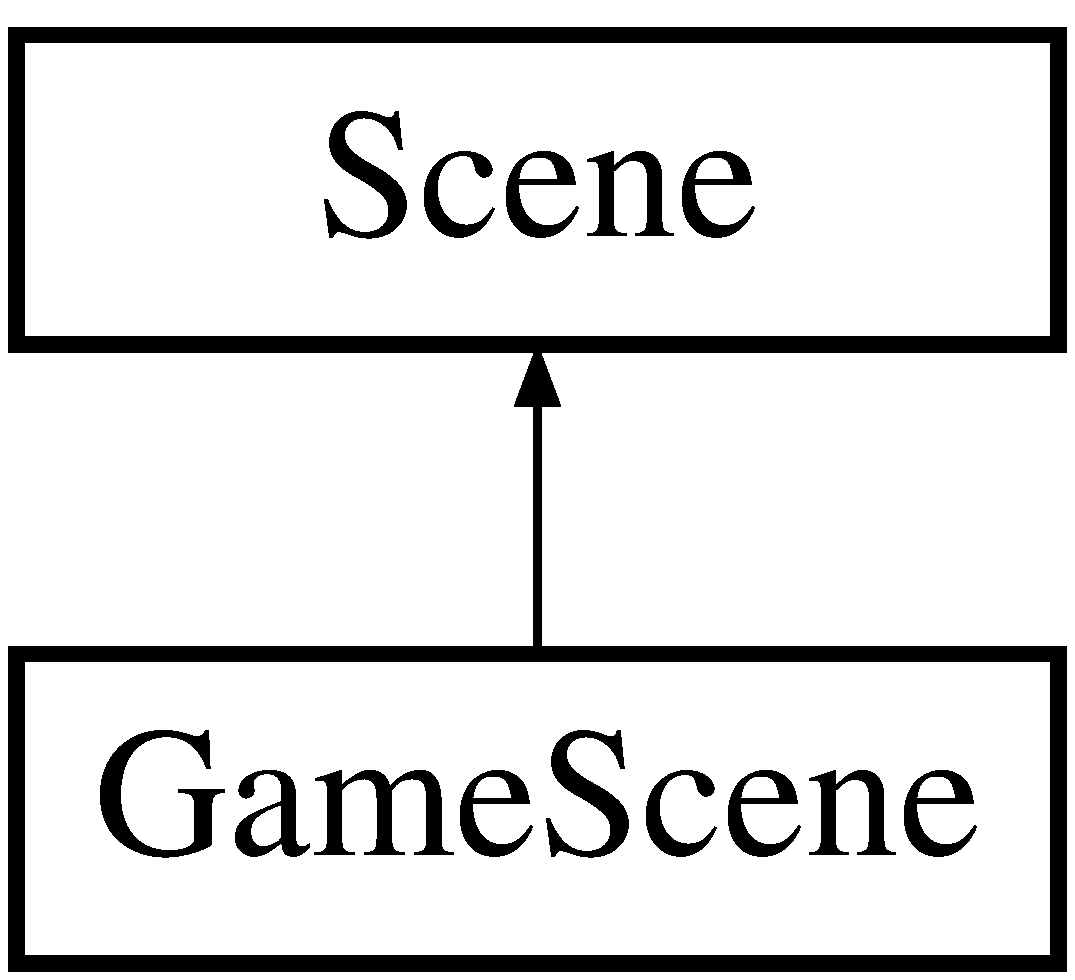
\includegraphics[height=2.000000cm]{class_game_scene}
\end{center}
\end{figure}
\subsection*{Public Member Functions}
\begin{DoxyCompactItemize}
\item 
\hyperlink{class_game_scene_a09ae1eacea6ea92074d008c016e0ed1f}{Game\+Scene} (\hyperlink{class_scene_stack}{Scene\+Stack} \&stack, \hyperlink{struct_scene_1_1_context}{Context} context)
\item 
\hyperlink{class_game_scene_add5bc48c372aaa7f526c02558a8adf00}{$\sim$\+Game\+Scene} ()
\item 
virtual void \hyperlink{class_game_scene_ae9eb60cbb8fa55eeb07b951e3d83f426}{draw} ()
\item 
virtual bool \hyperlink{class_game_scene_ae54628d2f041bcad66242584b2db10d6}{update} (sf\+::\+Time delta\+Time)
\item 
virtual bool \hyperlink{class_game_scene_aa494372b1f451f3c3a268558fddb30f2}{handle\+Event} (const sf\+::\+Event \&event)
\item 
bool \hyperlink{class_game_scene_a6cef526c611ff96b8771e60eea8ccebe}{check\+Enemies\+Alive} ()
\item 
void \hyperlink{class_game_scene_a67664e1bbce6bec9eda855a9b109d9ec}{setup\+Shockwave} (sf\+::\+Vector2f player\+Pos)
\item 
void \hyperlink{class_game_scene_aca0b30f731595929fb7182e2f65941b1}{setup\+Ripple} (sf\+::\+Vector2f player\+Pos)
\item 
void \hyperlink{class_game_scene_a030583d6469d9f44fda3fc5777c46a08}{screen\+Switch} (std\+::vector$<$ \hyperlink{class_bullet}{Bullet} $\ast$$>$ bullets)
\end{DoxyCompactItemize}
\subsection*{Additional Inherited Members}


\subsection{Detailed Description}
Handles everything that occurs during the game. 



\subsection{Constructor \& Destructor Documentation}
\mbox{\Hypertarget{class_game_scene_a09ae1eacea6ea92074d008c016e0ed1f}\label{class_game_scene_a09ae1eacea6ea92074d008c016e0ed1f}} 
\index{Game\+Scene@{Game\+Scene}!Game\+Scene@{Game\+Scene}}
\index{Game\+Scene@{Game\+Scene}!Game\+Scene@{Game\+Scene}}
\subsubsection{\texorpdfstring{Game\+Scene()}{GameScene()}}
{\footnotesize\ttfamily Game\+Scene\+::\+Game\+Scene (\begin{DoxyParamCaption}\item[{\hyperlink{class_scene_stack}{Scene\+Stack} \&}]{stack,  }\item[{\hyperlink{struct_scene_1_1_context}{Context}}]{context }\end{DoxyParamCaption})}

\mbox{\Hypertarget{class_game_scene_add5bc48c372aaa7f526c02558a8adf00}\label{class_game_scene_add5bc48c372aaa7f526c02558a8adf00}} 
\index{Game\+Scene@{Game\+Scene}!````~Game\+Scene@{$\sim$\+Game\+Scene}}
\index{````~Game\+Scene@{$\sim$\+Game\+Scene}!Game\+Scene@{Game\+Scene}}
\subsubsection{\texorpdfstring{$\sim$\+Game\+Scene()}{~GameScene()}}
{\footnotesize\ttfamily Game\+Scene\+::$\sim$\+Game\+Scene (\begin{DoxyParamCaption}{ }\end{DoxyParamCaption})}



\subsection{Member Function Documentation}
\mbox{\Hypertarget{class_game_scene_a6cef526c611ff96b8771e60eea8ccebe}\label{class_game_scene_a6cef526c611ff96b8771e60eea8ccebe}} 
\index{Game\+Scene@{Game\+Scene}!check\+Enemies\+Alive@{check\+Enemies\+Alive}}
\index{check\+Enemies\+Alive@{check\+Enemies\+Alive}!Game\+Scene@{Game\+Scene}}
\subsubsection{\texorpdfstring{check\+Enemies\+Alive()}{checkEnemiesAlive()}}
{\footnotesize\ttfamily bool Game\+Scene\+::check\+Enemies\+Alive (\begin{DoxyParamCaption}{ }\end{DoxyParamCaption})}

Check to see if all enemies have been killed, complete game when all enemies are dead \mbox{\Hypertarget{class_game_scene_ae9eb60cbb8fa55eeb07b951e3d83f426}\label{class_game_scene_ae9eb60cbb8fa55eeb07b951e3d83f426}} 
\index{Game\+Scene@{Game\+Scene}!draw@{draw}}
\index{draw@{draw}!Game\+Scene@{Game\+Scene}}
\subsubsection{\texorpdfstring{draw()}{draw()}}
{\footnotesize\ttfamily void Game\+Scene\+::draw (\begin{DoxyParamCaption}{ }\end{DoxyParamCaption})\hspace{0.3cm}{\ttfamily [virtual]}}

Manages drawing all game entities in the gamescene 

Implements \hyperlink{class_scene_a789c16961aa1e316b2a4a05b95187546}{Scene}.

\mbox{\Hypertarget{class_game_scene_aa494372b1f451f3c3a268558fddb30f2}\label{class_game_scene_aa494372b1f451f3c3a268558fddb30f2}} 
\index{Game\+Scene@{Game\+Scene}!handle\+Event@{handle\+Event}}
\index{handle\+Event@{handle\+Event}!Game\+Scene@{Game\+Scene}}
\subsubsection{\texorpdfstring{handle\+Event()}{handleEvent()}}
{\footnotesize\ttfamily bool Game\+Scene\+::handle\+Event (\begin{DoxyParamCaption}\item[{const sf\+::\+Event \&}]{event }\end{DoxyParamCaption})\hspace{0.3cm}{\ttfamily [virtual]}}

Manages handle input for the gamescene 

Implements \hyperlink{class_scene_af25e4d2c998aca4e95899fb67488e815}{Scene}.

\mbox{\Hypertarget{class_game_scene_a030583d6469d9f44fda3fc5777c46a08}\label{class_game_scene_a030583d6469d9f44fda3fc5777c46a08}} 
\index{Game\+Scene@{Game\+Scene}!screen\+Switch@{screen\+Switch}}
\index{screen\+Switch@{screen\+Switch}!Game\+Scene@{Game\+Scene}}
\subsubsection{\texorpdfstring{screen\+Switch()}{screenSwitch()}}
{\footnotesize\ttfamily void Game\+Scene\+::screen\+Switch (\begin{DoxyParamCaption}\item[{std\+::vector$<$ \hyperlink{class_bullet}{Bullet} $\ast$$>$}]{bullets }\end{DoxyParamCaption})}

When the player screen swap from onside to the other any enemy with in the players view gets swapped also \mbox{\Hypertarget{class_game_scene_aca0b30f731595929fb7182e2f65941b1}\label{class_game_scene_aca0b30f731595929fb7182e2f65941b1}} 
\index{Game\+Scene@{Game\+Scene}!setup\+Ripple@{setup\+Ripple}}
\index{setup\+Ripple@{setup\+Ripple}!Game\+Scene@{Game\+Scene}}
\subsubsection{\texorpdfstring{setup\+Ripple()}{setupRipple()}}
{\footnotesize\ttfamily void Game\+Scene\+::setup\+Ripple (\begin{DoxyParamCaption}\item[{sf\+::\+Vector2f}]{player\+Pos }\end{DoxyParamCaption})}

Sets up the ripple/teleporting shader effect using players current position \mbox{\Hypertarget{class_game_scene_a67664e1bbce6bec9eda855a9b109d9ec}\label{class_game_scene_a67664e1bbce6bec9eda855a9b109d9ec}} 
\index{Game\+Scene@{Game\+Scene}!setup\+Shockwave@{setup\+Shockwave}}
\index{setup\+Shockwave@{setup\+Shockwave}!Game\+Scene@{Game\+Scene}}
\subsubsection{\texorpdfstring{setup\+Shockwave()}{setupShockwave()}}
{\footnotesize\ttfamily void Game\+Scene\+::setup\+Shockwave (\begin{DoxyParamCaption}\item[{sf\+::\+Vector2f}]{player\+Pos }\end{DoxyParamCaption})}

Sets up the shockwave/smartbomb shader effect using players current position \mbox{\Hypertarget{class_game_scene_ae54628d2f041bcad66242584b2db10d6}\label{class_game_scene_ae54628d2f041bcad66242584b2db10d6}} 
\index{Game\+Scene@{Game\+Scene}!update@{update}}
\index{update@{update}!Game\+Scene@{Game\+Scene}}
\subsubsection{\texorpdfstring{update()}{update()}}
{\footnotesize\ttfamily bool Game\+Scene\+::update (\begin{DoxyParamCaption}\item[{sf\+::\+Time}]{delta\+Time }\end{DoxyParamCaption})\hspace{0.3cm}{\ttfamily [virtual]}}

Manages the update of all game entities in the gamescene 

Implements \hyperlink{class_scene_a72683c984a1da2ce4f757705e93730f2}{Scene}.



The documentation for this class was generated from the following files\+:\begin{DoxyCompactItemize}
\item 
S\+F\+M\+L Engine/\hyperlink{_game_scene_8h}{Game\+Scene.\+h}\item 
S\+F\+M\+L Engine/\hyperlink{_game_scene_8cpp}{Game\+Scene.\+cpp}\end{DoxyCompactItemize}

\hypertarget{class_helper}{}\section{Helper Class Reference}
\label{class_helper}\index{Helper@{Helper}}


{\ttfamily \#include $<$Helper.\+h$>$}

\subsection*{Static Public Member Functions}
\begin{DoxyCompactItemize}
\item 
static float \hyperlink{class_helper_ad2b13a8d9fff4f913a57db9903df7709}{Length} (sf\+::\+Vector2f v)
\item 
static float \hyperlink{class_helper_ad6c52dd3a1875fbffc268196a6a6a887}{Length\+Squared} (sf\+::\+Vector2f v)
\item 
static sf\+::\+Vector2f \hyperlink{class_helper_a1a431211d082593425ccfafe077dd5bc}{Div\+Scaler} (sf\+::\+Vector2f v, float s)
\item 
static float \hyperlink{class_helper_aabf497b73c8aedbaf02b0f579ce73704}{Distance} (sf\+::\+Vector2f v, sf\+::\+Vector2f v2)
\item 
static sf\+::\+Vector2f \hyperlink{class_helper_a7565c8f3c91f44e139d7a4aaef6e0e34}{Normalize} (sf\+::\+Vector2f v)
\item 
static float \hyperlink{class_helper_a7a1497494599fe9b5bc68718c812d903}{dot\+Product} (sf\+::\+Vector2f v, sf\+::\+Vector2f v2)
\item 
static float \hyperlink{class_helper_a0a21ce7bbd26f902abbe5fe078b20044}{angle\+Between} (sf\+::\+Vector2f v, sf\+::\+Vector2f v2)
\end{DoxyCompactItemize}


\subsection{Member Function Documentation}
\mbox{\Hypertarget{class_helper_a0a21ce7bbd26f902abbe5fe078b20044}\label{class_helper_a0a21ce7bbd26f902abbe5fe078b20044}} 
\index{Helper@{Helper}!angle\+Between@{angle\+Between}}
\index{angle\+Between@{angle\+Between}!Helper@{Helper}}
\subsubsection{\texorpdfstring{angle\+Between()}{angleBetween()}}
{\footnotesize\ttfamily static float Helper\+::angle\+Between (\begin{DoxyParamCaption}\item[{sf\+::\+Vector2f}]{v,  }\item[{sf\+::\+Vector2f}]{v2 }\end{DoxyParamCaption})\hspace{0.3cm}{\ttfamily [inline]}, {\ttfamily [static]}}

\mbox{\Hypertarget{class_helper_aabf497b73c8aedbaf02b0f579ce73704}\label{class_helper_aabf497b73c8aedbaf02b0f579ce73704}} 
\index{Helper@{Helper}!Distance@{Distance}}
\index{Distance@{Distance}!Helper@{Helper}}
\subsubsection{\texorpdfstring{Distance()}{Distance()}}
{\footnotesize\ttfamily static float Helper\+::\+Distance (\begin{DoxyParamCaption}\item[{sf\+::\+Vector2f}]{v,  }\item[{sf\+::\+Vector2f}]{v2 }\end{DoxyParamCaption})\hspace{0.3cm}{\ttfamily [inline]}, {\ttfamily [static]}}

\mbox{\Hypertarget{class_helper_a1a431211d082593425ccfafe077dd5bc}\label{class_helper_a1a431211d082593425ccfafe077dd5bc}} 
\index{Helper@{Helper}!Div\+Scaler@{Div\+Scaler}}
\index{Div\+Scaler@{Div\+Scaler}!Helper@{Helper}}
\subsubsection{\texorpdfstring{Div\+Scaler()}{DivScaler()}}
{\footnotesize\ttfamily static sf\+::\+Vector2f Helper\+::\+Div\+Scaler (\begin{DoxyParamCaption}\item[{sf\+::\+Vector2f}]{v,  }\item[{float}]{s }\end{DoxyParamCaption})\hspace{0.3cm}{\ttfamily [inline]}, {\ttfamily [static]}}

\mbox{\Hypertarget{class_helper_a7a1497494599fe9b5bc68718c812d903}\label{class_helper_a7a1497494599fe9b5bc68718c812d903}} 
\index{Helper@{Helper}!dot\+Product@{dot\+Product}}
\index{dot\+Product@{dot\+Product}!Helper@{Helper}}
\subsubsection{\texorpdfstring{dot\+Product()}{dotProduct()}}
{\footnotesize\ttfamily static float Helper\+::dot\+Product (\begin{DoxyParamCaption}\item[{sf\+::\+Vector2f}]{v,  }\item[{sf\+::\+Vector2f}]{v2 }\end{DoxyParamCaption})\hspace{0.3cm}{\ttfamily [inline]}, {\ttfamily [static]}}

\mbox{\Hypertarget{class_helper_ad2b13a8d9fff4f913a57db9903df7709}\label{class_helper_ad2b13a8d9fff4f913a57db9903df7709}} 
\index{Helper@{Helper}!Length@{Length}}
\index{Length@{Length}!Helper@{Helper}}
\subsubsection{\texorpdfstring{Length()}{Length()}}
{\footnotesize\ttfamily static float Helper\+::\+Length (\begin{DoxyParamCaption}\item[{sf\+::\+Vector2f}]{v }\end{DoxyParamCaption})\hspace{0.3cm}{\ttfamily [inline]}, {\ttfamily [static]}}

\mbox{\Hypertarget{class_helper_ad6c52dd3a1875fbffc268196a6a6a887}\label{class_helper_ad6c52dd3a1875fbffc268196a6a6a887}} 
\index{Helper@{Helper}!Length\+Squared@{Length\+Squared}}
\index{Length\+Squared@{Length\+Squared}!Helper@{Helper}}
\subsubsection{\texorpdfstring{Length\+Squared()}{LengthSquared()}}
{\footnotesize\ttfamily static float Helper\+::\+Length\+Squared (\begin{DoxyParamCaption}\item[{sf\+::\+Vector2f}]{v }\end{DoxyParamCaption})\hspace{0.3cm}{\ttfamily [inline]}, {\ttfamily [static]}}

\mbox{\Hypertarget{class_helper_a7565c8f3c91f44e139d7a4aaef6e0e34}\label{class_helper_a7565c8f3c91f44e139d7a4aaef6e0e34}} 
\index{Helper@{Helper}!Normalize@{Normalize}}
\index{Normalize@{Normalize}!Helper@{Helper}}
\subsubsection{\texorpdfstring{Normalize()}{Normalize()}}
{\footnotesize\ttfamily static sf\+::\+Vector2f Helper\+::\+Normalize (\begin{DoxyParamCaption}\item[{sf\+::\+Vector2f}]{v }\end{DoxyParamCaption})\hspace{0.3cm}{\ttfamily [inline]}, {\ttfamily [static]}}



The documentation for this class was generated from the following file\+:\begin{DoxyCompactItemize}
\item 
S\+F\+M\+L Engine/\hyperlink{_helper_8h}{Helper.\+h}\end{DoxyCompactItemize}

\hypertarget{class_pause_scene}{}\section{Pause\+Scene Class Reference}
\label{class_pause_scene}\index{Pause\+Scene@{Pause\+Scene}}


{\ttfamily \#include $<$Pause\+Scene.\+h$>$}

Inheritance diagram for Pause\+Scene\+:\begin{figure}[H]
\begin{center}
\leavevmode
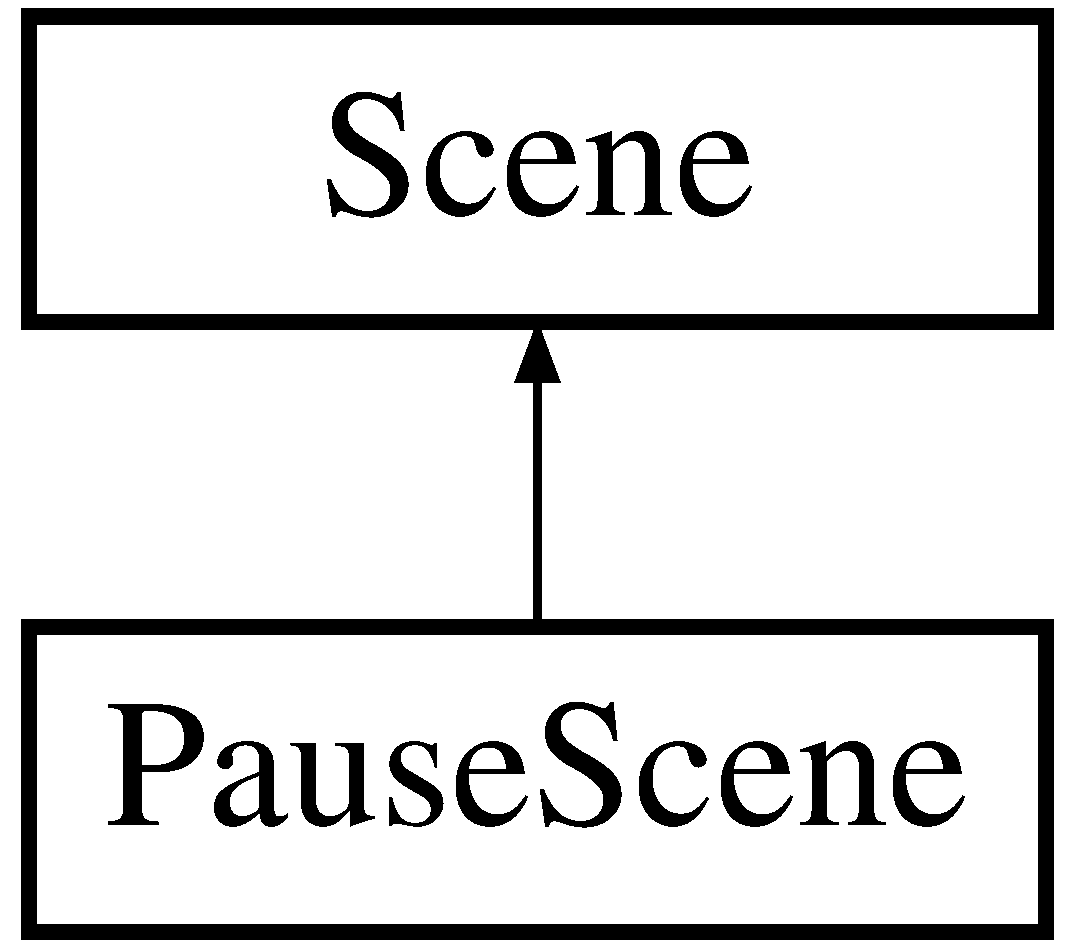
\includegraphics[height=2.000000cm]{class_pause_scene}
\end{center}
\end{figure}
\subsection*{Public Member Functions}
\begin{DoxyCompactItemize}
\item 
\hyperlink{class_pause_scene_a65ac2aa9fca0b1027481e60417749c4f}{Pause\+Scene} (\hyperlink{class_scene_stack}{Scene\+Stack} \&stack, \hyperlink{struct_scene_1_1_context}{Context} context)
\item 
void \hyperlink{class_pause_scene_abfd1398a064a83b3ae6ac5fd98aebf05}{draw} () override
\item 
bool \hyperlink{class_pause_scene_a8504260009b4dfb2380785e938e60b4b}{update} (sf\+::\+Time delta\+Time) override
\item 
bool \hyperlink{class_pause_scene_adeb06e37e0a2afa297ddbe795c3cbe94}{handle\+Event} (const sf\+::\+Event \&event) override
\end{DoxyCompactItemize}
\subsection*{Additional Inherited Members}


\subsection{Constructor \& Destructor Documentation}
\mbox{\Hypertarget{class_pause_scene_a65ac2aa9fca0b1027481e60417749c4f}\label{class_pause_scene_a65ac2aa9fca0b1027481e60417749c4f}} 
\index{Pause\+Scene@{Pause\+Scene}!Pause\+Scene@{Pause\+Scene}}
\index{Pause\+Scene@{Pause\+Scene}!Pause\+Scene@{Pause\+Scene}}
\subsubsection{\texorpdfstring{Pause\+Scene()}{PauseScene()}}
{\footnotesize\ttfamily Pause\+Scene\+::\+Pause\+Scene (\begin{DoxyParamCaption}\item[{\hyperlink{class_scene_stack}{Scene\+Stack} \&}]{stack,  }\item[{\hyperlink{struct_scene_1_1_context}{Context}}]{context }\end{DoxyParamCaption})}



\subsection{Member Function Documentation}
\mbox{\Hypertarget{class_pause_scene_abfd1398a064a83b3ae6ac5fd98aebf05}\label{class_pause_scene_abfd1398a064a83b3ae6ac5fd98aebf05}} 
\index{Pause\+Scene@{Pause\+Scene}!draw@{draw}}
\index{draw@{draw}!Pause\+Scene@{Pause\+Scene}}
\subsubsection{\texorpdfstring{draw()}{draw()}}
{\footnotesize\ttfamily void Pause\+Scene\+::draw (\begin{DoxyParamCaption}{ }\end{DoxyParamCaption})\hspace{0.3cm}{\ttfamily [override]}, {\ttfamily [virtual]}}



Implements \hyperlink{class_scene_a789c16961aa1e316b2a4a05b95187546}{Scene}.

\mbox{\Hypertarget{class_pause_scene_adeb06e37e0a2afa297ddbe795c3cbe94}\label{class_pause_scene_adeb06e37e0a2afa297ddbe795c3cbe94}} 
\index{Pause\+Scene@{Pause\+Scene}!handle\+Event@{handle\+Event}}
\index{handle\+Event@{handle\+Event}!Pause\+Scene@{Pause\+Scene}}
\subsubsection{\texorpdfstring{handle\+Event()}{handleEvent()}}
{\footnotesize\ttfamily bool Pause\+Scene\+::handle\+Event (\begin{DoxyParamCaption}\item[{const sf\+::\+Event \&}]{event }\end{DoxyParamCaption})\hspace{0.3cm}{\ttfamily [override]}, {\ttfamily [virtual]}}



Implements \hyperlink{class_scene_af25e4d2c998aca4e95899fb67488e815}{Scene}.

\mbox{\Hypertarget{class_pause_scene_a8504260009b4dfb2380785e938e60b4b}\label{class_pause_scene_a8504260009b4dfb2380785e938e60b4b}} 
\index{Pause\+Scene@{Pause\+Scene}!update@{update}}
\index{update@{update}!Pause\+Scene@{Pause\+Scene}}
\subsubsection{\texorpdfstring{update()}{update()}}
{\footnotesize\ttfamily bool Pause\+Scene\+::update (\begin{DoxyParamCaption}\item[{sf\+::\+Time}]{delta\+Time }\end{DoxyParamCaption})\hspace{0.3cm}{\ttfamily [override]}, {\ttfamily [virtual]}}



Implements \hyperlink{class_scene_a72683c984a1da2ce4f757705e93730f2}{Scene}.



The documentation for this class was generated from the following files\+:\begin{DoxyCompactItemize}
\item 
S\+F\+M\+L Engine/\hyperlink{_pause_scene_8h}{Pause\+Scene.\+h}\item 
S\+F\+M\+L Engine/\hyperlink{_pause_scene_8cpp}{Pause\+Scene.\+cpp}\end{DoxyCompactItemize}

\hypertarget{class_player}{}\section{Player Class Reference}
\label{class_player}\index{Player@{Player}}


Handles all the properties and responsibilities of the player.  




{\ttfamily \#include $<$Player.\+h$>$}

\subsection*{Public Types}
\begin{DoxyCompactItemize}
\item 
enum \hyperlink{class_player_afd539a18e0e4c3bbf07c820914c0511e}{Smart\+Bomb} \{ \hyperlink{class_player_afd539a18e0e4c3bbf07c820914c0511ea62fc7d85d72db94f418347b5e3a25d28}{Ready}, 
\hyperlink{class_player_afd539a18e0e4c3bbf07c820914c0511ea86d19f9b31edc54d666dd859955f2ae4}{Charging}, 
\hyperlink{class_player_afd539a18e0e4c3bbf07c820914c0511eaefb39c3c6842102cf73bd0203e41b338}{Fired}, 
\hyperlink{class_player_afd539a18e0e4c3bbf07c820914c0511ea0dc1ade8c7310201d494698675fd011d}{Disable}
 \}
\end{DoxyCompactItemize}
\subsection*{Public Member Functions}
\begin{DoxyCompactItemize}
\item 
\hyperlink{class_player_affe0cc3cb714f6deb4e62f0c0d3f1fd8}{Player} ()
\item 
\hyperlink{class_player_a749d2c00e1fe0f5c2746f7505a58c062}{$\sim$\+Player} ()
\item 
void \hyperlink{class_player_ad088063876ac0e5c3eb59fc7c4806929}{init} (sf\+::\+Texture \&tex, sf\+::\+Vector2f pos, sf\+::\+Vector2i tp\+Bounds)
\item 
void \hyperlink{class_player_aeb1ca63f5401afa5d6aef2f308481672}{update} (sf\+::\+Time delta\+Time)
\item 
void \hyperlink{class_player_aab4ff61041f937e6c3d560863fa46f56}{Move} (sf\+::\+Time delta\+Time)
\item 
\hyperlink{class_animated_sprite}{Animated\+Sprite} \hyperlink{class_player_af9e361fd707a32d86ff1a0f75fb2c3b2}{draw} ()
\item 
void \hyperlink{class_player_ad975c53e4e2e21b597079e59c1ed0262}{teleport} (sf\+::\+Time delta\+Time)
\item 
int \hyperlink{class_player_a995b03fe2b8f0b47aa526c975a3b8254}{get\+Teleport} ()
\item 
void \hyperlink{class_player_a805a8d4ae2c5eddaee1ff7c716467f2c}{disable\+Teleporter} ()
\item 
int \hyperlink{class_player_a5aaef7be6b70ec6069a861add36b5e2c}{get\+Smart\+Bomb\+State} ()
\item 
void \hyperlink{class_player_a2c704d0bed9de1dc0b3512113f42bb97}{charge\+Smart\+Bomb} ()
\item 
void \hyperlink{class_player_a41a1a1a4f50f7a878ee22c92b42fd2b1}{update\+Smart\+Bomb} (sf\+::\+Time delta\+Time)
\item 
void \hyperlink{class_player_a065d28e46d0660eff17bad53f2efd622}{set\+Damage} (int damage)
\item 
int \hyperlink{class_player_abcb15d249bed9a4ab0ab86b52b0d747a}{get\+Health} ()
\item 
int \hyperlink{class_player_a96b2c2aa27ba5d756b12fddb2a841cc8}{get\+Radius} ()
\item 
bool \hyperlink{class_player_a98dff5ba148838f3db6d9934048c33d9}{game\+Over} ()
\item 
sf\+::\+Vector2f \hyperlink{class_player_a23356f99a9de86d3d47eadb679b332dc}{get\+Position} ()
\item 
void \hyperlink{class_player_a04a1bb340ea6d425fb2927c397e96e4e}{set\+Position} (sf\+::\+Vector2f pos)
\item 
sf\+::\+Circle\+Shape \hyperlink{class_player_ae47cf3c74c1e396d82c3266290871852}{draw\+Player\+Outline} ()
\item 
sf\+::\+Vector2f \hyperlink{class_player_a0ec9b337a29a388ca7ce6dc9de93ca76}{get\+Vel} ()
\item 
sf\+::\+Vector2f \hyperlink{class_player_acd90a76e6bf73c5a7d2ff168965c3467}{get\+Accel} ()
\end{DoxyCompactItemize}
\subsection*{Public Attributes}
\begin{DoxyCompactItemize}
\item 
\hyperlink{class_animated_sprite}{Animated\+Sprite} \hyperlink{class_player_a6d6dfb4b46e5aa9eac78fd8cced73825}{m\+\_\+animated\+Sprite}
\item 
float \hyperlink{class_player_adb6552419db92fdbc9aeda36e807c6ec}{m\+\_\+smart\+Bomb\+Timer}
\end{DoxyCompactItemize}


\subsection{Detailed Description}
Handles all the properties and responsibilities of the player. 



\subsection{Member Enumeration Documentation}
\mbox{\Hypertarget{class_player_afd539a18e0e4c3bbf07c820914c0511e}\label{class_player_afd539a18e0e4c3bbf07c820914c0511e}} 
\index{Player@{Player}!Smart\+Bomb@{Smart\+Bomb}}
\index{Smart\+Bomb@{Smart\+Bomb}!Player@{Player}}
\subsubsection{\texorpdfstring{Smart\+Bomb}{SmartBomb}}
{\footnotesize\ttfamily enum \hyperlink{class_player_afd539a18e0e4c3bbf07c820914c0511e}{Player\+::\+Smart\+Bomb}}

\begin{DoxyEnumFields}{Enumerator}
\raisebox{\heightof{T}}[0pt][0pt]{\index{Ready@{Ready}!Player@{Player}}\index{Player@{Player}!Ready@{Ready}}}\mbox{\Hypertarget{class_player_afd539a18e0e4c3bbf07c820914c0511ea62fc7d85d72db94f418347b5e3a25d28}\label{class_player_afd539a18e0e4c3bbf07c820914c0511ea62fc7d85d72db94f418347b5e3a25d28}} 
Ready&\\
\hline

\raisebox{\heightof{T}}[0pt][0pt]{\index{Charging@{Charging}!Player@{Player}}\index{Player@{Player}!Charging@{Charging}}}\mbox{\Hypertarget{class_player_afd539a18e0e4c3bbf07c820914c0511ea86d19f9b31edc54d666dd859955f2ae4}\label{class_player_afd539a18e0e4c3bbf07c820914c0511ea86d19f9b31edc54d666dd859955f2ae4}} 
Charging&\\
\hline

\raisebox{\heightof{T}}[0pt][0pt]{\index{Fired@{Fired}!Player@{Player}}\index{Player@{Player}!Fired@{Fired}}}\mbox{\Hypertarget{class_player_afd539a18e0e4c3bbf07c820914c0511eaefb39c3c6842102cf73bd0203e41b338}\label{class_player_afd539a18e0e4c3bbf07c820914c0511eaefb39c3c6842102cf73bd0203e41b338}} 
Fired&\\
\hline

\raisebox{\heightof{T}}[0pt][0pt]{\index{Disable@{Disable}!Player@{Player}}\index{Player@{Player}!Disable@{Disable}}}\mbox{\Hypertarget{class_player_afd539a18e0e4c3bbf07c820914c0511ea0dc1ade8c7310201d494698675fd011d}\label{class_player_afd539a18e0e4c3bbf07c820914c0511ea0dc1ade8c7310201d494698675fd011d}} 
Disable&\\
\hline

\end{DoxyEnumFields}


\subsection{Constructor \& Destructor Documentation}
\mbox{\Hypertarget{class_player_affe0cc3cb714f6deb4e62f0c0d3f1fd8}\label{class_player_affe0cc3cb714f6deb4e62f0c0d3f1fd8}} 
\index{Player@{Player}!Player@{Player}}
\index{Player@{Player}!Player@{Player}}
\subsubsection{\texorpdfstring{Player()}{Player()}}
{\footnotesize\ttfamily Player\+::\+Player (\begin{DoxyParamCaption}{ }\end{DoxyParamCaption})}

\mbox{\Hypertarget{class_player_a749d2c00e1fe0f5c2746f7505a58c062}\label{class_player_a749d2c00e1fe0f5c2746f7505a58c062}} 
\index{Player@{Player}!````~Player@{$\sim$\+Player}}
\index{````~Player@{$\sim$\+Player}!Player@{Player}}
\subsubsection{\texorpdfstring{$\sim$\+Player()}{~Player()}}
{\footnotesize\ttfamily Player\+::$\sim$\+Player (\begin{DoxyParamCaption}{ }\end{DoxyParamCaption})}



\subsection{Member Function Documentation}
\mbox{\Hypertarget{class_player_a2c704d0bed9de1dc0b3512113f42bb97}\label{class_player_a2c704d0bed9de1dc0b3512113f42bb97}} 
\index{Player@{Player}!charge\+Smart\+Bomb@{charge\+Smart\+Bomb}}
\index{charge\+Smart\+Bomb@{charge\+Smart\+Bomb}!Player@{Player}}
\subsubsection{\texorpdfstring{charge\+Smart\+Bomb()}{chargeSmartBomb()}}
{\footnotesize\ttfamily void Player\+::charge\+Smart\+Bomb (\begin{DoxyParamCaption}{ }\end{DoxyParamCaption})}

\mbox{\Hypertarget{class_player_a805a8d4ae2c5eddaee1ff7c716467f2c}\label{class_player_a805a8d4ae2c5eddaee1ff7c716467f2c}} 
\index{Player@{Player}!disable\+Teleporter@{disable\+Teleporter}}
\index{disable\+Teleporter@{disable\+Teleporter}!Player@{Player}}
\subsubsection{\texorpdfstring{disable\+Teleporter()}{disableTeleporter()}}
{\footnotesize\ttfamily void Player\+::disable\+Teleporter (\begin{DoxyParamCaption}{ }\end{DoxyParamCaption})}

\mbox{\Hypertarget{class_player_af9e361fd707a32d86ff1a0f75fb2c3b2}\label{class_player_af9e361fd707a32d86ff1a0f75fb2c3b2}} 
\index{Player@{Player}!draw@{draw}}
\index{draw@{draw}!Player@{Player}}
\subsubsection{\texorpdfstring{draw()}{draw()}}
{\footnotesize\ttfamily \hyperlink{class_animated_sprite}{Animated\+Sprite} Player\+::draw (\begin{DoxyParamCaption}{ }\end{DoxyParamCaption})}

\mbox{\Hypertarget{class_player_ae47cf3c74c1e396d82c3266290871852}\label{class_player_ae47cf3c74c1e396d82c3266290871852}} 
\index{Player@{Player}!draw\+Player\+Outline@{draw\+Player\+Outline}}
\index{draw\+Player\+Outline@{draw\+Player\+Outline}!Player@{Player}}
\subsubsection{\texorpdfstring{draw\+Player\+Outline()}{drawPlayerOutline()}}
{\footnotesize\ttfamily sf\+::\+Circle\+Shape Player\+::draw\+Player\+Outline (\begin{DoxyParamCaption}{ }\end{DoxyParamCaption})}

\mbox{\Hypertarget{class_player_a98dff5ba148838f3db6d9934048c33d9}\label{class_player_a98dff5ba148838f3db6d9934048c33d9}} 
\index{Player@{Player}!game\+Over@{game\+Over}}
\index{game\+Over@{game\+Over}!Player@{Player}}
\subsubsection{\texorpdfstring{game\+Over()}{gameOver()}}
{\footnotesize\ttfamily bool Player\+::game\+Over (\begin{DoxyParamCaption}{ }\end{DoxyParamCaption})}

\mbox{\Hypertarget{class_player_acd90a76e6bf73c5a7d2ff168965c3467}\label{class_player_acd90a76e6bf73c5a7d2ff168965c3467}} 
\index{Player@{Player}!get\+Accel@{get\+Accel}}
\index{get\+Accel@{get\+Accel}!Player@{Player}}
\subsubsection{\texorpdfstring{get\+Accel()}{getAccel()}}
{\footnotesize\ttfamily sf\+::\+Vector2f Player\+::get\+Accel (\begin{DoxyParamCaption}{ }\end{DoxyParamCaption})}

\mbox{\Hypertarget{class_player_abcb15d249bed9a4ab0ab86b52b0d747a}\label{class_player_abcb15d249bed9a4ab0ab86b52b0d747a}} 
\index{Player@{Player}!get\+Health@{get\+Health}}
\index{get\+Health@{get\+Health}!Player@{Player}}
\subsubsection{\texorpdfstring{get\+Health()}{getHealth()}}
{\footnotesize\ttfamily int Player\+::get\+Health (\begin{DoxyParamCaption}{ }\end{DoxyParamCaption})}

\mbox{\Hypertarget{class_player_a23356f99a9de86d3d47eadb679b332dc}\label{class_player_a23356f99a9de86d3d47eadb679b332dc}} 
\index{Player@{Player}!get\+Position@{get\+Position}}
\index{get\+Position@{get\+Position}!Player@{Player}}
\subsubsection{\texorpdfstring{get\+Position()}{getPosition()}}
{\footnotesize\ttfamily sf\+::\+Vector2f Player\+::get\+Position (\begin{DoxyParamCaption}{ }\end{DoxyParamCaption})}

\mbox{\Hypertarget{class_player_a96b2c2aa27ba5d756b12fddb2a841cc8}\label{class_player_a96b2c2aa27ba5d756b12fddb2a841cc8}} 
\index{Player@{Player}!get\+Radius@{get\+Radius}}
\index{get\+Radius@{get\+Radius}!Player@{Player}}
\subsubsection{\texorpdfstring{get\+Radius()}{getRadius()}}
{\footnotesize\ttfamily int Player\+::get\+Radius (\begin{DoxyParamCaption}{ }\end{DoxyParamCaption})}

\mbox{\Hypertarget{class_player_a5aaef7be6b70ec6069a861add36b5e2c}\label{class_player_a5aaef7be6b70ec6069a861add36b5e2c}} 
\index{Player@{Player}!get\+Smart\+Bomb\+State@{get\+Smart\+Bomb\+State}}
\index{get\+Smart\+Bomb\+State@{get\+Smart\+Bomb\+State}!Player@{Player}}
\subsubsection{\texorpdfstring{get\+Smart\+Bomb\+State()}{getSmartBombState()}}
{\footnotesize\ttfamily int Player\+::get\+Smart\+Bomb\+State (\begin{DoxyParamCaption}{ }\end{DoxyParamCaption})}

\mbox{\Hypertarget{class_player_a995b03fe2b8f0b47aa526c975a3b8254}\label{class_player_a995b03fe2b8f0b47aa526c975a3b8254}} 
\index{Player@{Player}!get\+Teleport@{get\+Teleport}}
\index{get\+Teleport@{get\+Teleport}!Player@{Player}}
\subsubsection{\texorpdfstring{get\+Teleport()}{getTeleport()}}
{\footnotesize\ttfamily int Player\+::get\+Teleport (\begin{DoxyParamCaption}{ }\end{DoxyParamCaption})}

\mbox{\Hypertarget{class_player_a0ec9b337a29a388ca7ce6dc9de93ca76}\label{class_player_a0ec9b337a29a388ca7ce6dc9de93ca76}} 
\index{Player@{Player}!get\+Vel@{get\+Vel}}
\index{get\+Vel@{get\+Vel}!Player@{Player}}
\subsubsection{\texorpdfstring{get\+Vel()}{getVel()}}
{\footnotesize\ttfamily sf\+::\+Vector2f Player\+::get\+Vel (\begin{DoxyParamCaption}{ }\end{DoxyParamCaption})}

\mbox{\Hypertarget{class_player_ad088063876ac0e5c3eb59fc7c4806929}\label{class_player_ad088063876ac0e5c3eb59fc7c4806929}} 
\index{Player@{Player}!init@{init}}
\index{init@{init}!Player@{Player}}
\subsubsection{\texorpdfstring{init()}{init()}}
{\footnotesize\ttfamily void Player\+::init (\begin{DoxyParamCaption}\item[{sf\+::\+Texture \&}]{tex,  }\item[{sf\+::\+Vector2f}]{pos,  }\item[{sf\+::\+Vector2i}]{tp\+Bounds }\end{DoxyParamCaption})}

\mbox{\Hypertarget{class_player_aab4ff61041f937e6c3d560863fa46f56}\label{class_player_aab4ff61041f937e6c3d560863fa46f56}} 
\index{Player@{Player}!Move@{Move}}
\index{Move@{Move}!Player@{Player}}
\subsubsection{\texorpdfstring{Move()}{Move()}}
{\footnotesize\ttfamily void Player\+::\+Move (\begin{DoxyParamCaption}\item[{sf\+::\+Time}]{delta\+Time }\end{DoxyParamCaption})}

\mbox{\Hypertarget{class_player_a065d28e46d0660eff17bad53f2efd622}\label{class_player_a065d28e46d0660eff17bad53f2efd622}} 
\index{Player@{Player}!set\+Damage@{set\+Damage}}
\index{set\+Damage@{set\+Damage}!Player@{Player}}
\subsubsection{\texorpdfstring{set\+Damage()}{setDamage()}}
{\footnotesize\ttfamily void Player\+::set\+Damage (\begin{DoxyParamCaption}\item[{int}]{damage }\end{DoxyParamCaption})}

\mbox{\Hypertarget{class_player_a04a1bb340ea6d425fb2927c397e96e4e}\label{class_player_a04a1bb340ea6d425fb2927c397e96e4e}} 
\index{Player@{Player}!set\+Position@{set\+Position}}
\index{set\+Position@{set\+Position}!Player@{Player}}
\subsubsection{\texorpdfstring{set\+Position()}{setPosition()}}
{\footnotesize\ttfamily void Player\+::set\+Position (\begin{DoxyParamCaption}\item[{sf\+::\+Vector2f}]{pos }\end{DoxyParamCaption})}

\mbox{\Hypertarget{class_player_ad975c53e4e2e21b597079e59c1ed0262}\label{class_player_ad975c53e4e2e21b597079e59c1ed0262}} 
\index{Player@{Player}!teleport@{teleport}}
\index{teleport@{teleport}!Player@{Player}}
\subsubsection{\texorpdfstring{teleport()}{teleport()}}
{\footnotesize\ttfamily void Player\+::teleport (\begin{DoxyParamCaption}\item[{sf\+::\+Time}]{delta\+Time }\end{DoxyParamCaption})}

\mbox{\Hypertarget{class_player_aeb1ca63f5401afa5d6aef2f308481672}\label{class_player_aeb1ca63f5401afa5d6aef2f308481672}} 
\index{Player@{Player}!update@{update}}
\index{update@{update}!Player@{Player}}
\subsubsection{\texorpdfstring{update()}{update()}}
{\footnotesize\ttfamily void Player\+::update (\begin{DoxyParamCaption}\item[{sf\+::\+Time}]{delta\+Time }\end{DoxyParamCaption})}

\mbox{\Hypertarget{class_player_a41a1a1a4f50f7a878ee22c92b42fd2b1}\label{class_player_a41a1a1a4f50f7a878ee22c92b42fd2b1}} 
\index{Player@{Player}!update\+Smart\+Bomb@{update\+Smart\+Bomb}}
\index{update\+Smart\+Bomb@{update\+Smart\+Bomb}!Player@{Player}}
\subsubsection{\texorpdfstring{update\+Smart\+Bomb()}{updateSmartBomb()}}
{\footnotesize\ttfamily void Player\+::update\+Smart\+Bomb (\begin{DoxyParamCaption}\item[{sf\+::\+Time}]{delta\+Time }\end{DoxyParamCaption})}



\subsection{Member Data Documentation}
\mbox{\Hypertarget{class_player_a6d6dfb4b46e5aa9eac78fd8cced73825}\label{class_player_a6d6dfb4b46e5aa9eac78fd8cced73825}} 
\index{Player@{Player}!m\+\_\+animated\+Sprite@{m\+\_\+animated\+Sprite}}
\index{m\+\_\+animated\+Sprite@{m\+\_\+animated\+Sprite}!Player@{Player}}
\subsubsection{\texorpdfstring{m\+\_\+animated\+Sprite}{m\_animatedSprite}}
{\footnotesize\ttfamily \hyperlink{class_animated_sprite}{Animated\+Sprite} Player\+::m\+\_\+animated\+Sprite}

\mbox{\Hypertarget{class_player_adb6552419db92fdbc9aeda36e807c6ec}\label{class_player_adb6552419db92fdbc9aeda36e807c6ec}} 
\index{Player@{Player}!m\+\_\+smart\+Bomb\+Timer@{m\+\_\+smart\+Bomb\+Timer}}
\index{m\+\_\+smart\+Bomb\+Timer@{m\+\_\+smart\+Bomb\+Timer}!Player@{Player}}
\subsubsection{\texorpdfstring{m\+\_\+smart\+Bomb\+Timer}{m\_smartBombTimer}}
{\footnotesize\ttfamily float Player\+::m\+\_\+smart\+Bomb\+Timer}



The documentation for this class was generated from the following files\+:\begin{DoxyCompactItemize}
\item 
S\+F\+M\+L Engine/\hyperlink{_player_8h}{Player.\+h}\item 
S\+F\+M\+L Engine/\hyperlink{_player_8cpp}{Player.\+cpp}\end{DoxyCompactItemize}

\hypertarget{class_resource_holder}{}\section{Resource\+Holder$<$ Resource, Identifier $>$ Class Template Reference}
\label{class_resource_holder}\index{Resource\+Holder$<$ Resource, Identifier $>$@{Resource\+Holder$<$ Resource, Identifier $>$}}


{\ttfamily \#include $<$Resource\+Holder.\+h$>$}

\subsection*{Public Member Functions}
\begin{DoxyCompactItemize}
\item 
void \hyperlink{class_resource_holder_accb6a2b6bd2da503ddfd57b5c0028a16}{load} (Identifier id, const std\+::string \&filename)
\item 
{\footnotesize template$<$typename Parameter $>$ }\\void \hyperlink{class_resource_holder_ae83a7a88b2b2a74b6143796eb4452110}{load} (Identifier id, const std\+::string \&filename, const Parameter \&second\+Param)
\item 
Resource \& \hyperlink{class_resource_holder_a6452638a75b6df7ea7d610f204632850}{get} (Identifier id)
\item 
const Resource \& \hyperlink{class_resource_holder_aaf453199dbdfb9b8395c52b29eb915c2}{get} (Identifier id) const
\end{DoxyCompactItemize}


\subsection{Member Function Documentation}
\mbox{\Hypertarget{class_resource_holder_a6452638a75b6df7ea7d610f204632850}\label{class_resource_holder_a6452638a75b6df7ea7d610f204632850}} 
\index{Resource\+Holder@{Resource\+Holder}!get@{get}}
\index{get@{get}!Resource\+Holder@{Resource\+Holder}}
\subsubsection{\texorpdfstring{get()}{get()}\hspace{0.1cm}{\footnotesize\ttfamily [1/2]}}
{\footnotesize\ttfamily template$<$typename Resource , typename Identifier$>$ \\
Resource \& \hyperlink{class_resource_holder}{Resource\+Holder}$<$ Resource, Identifier $>$\+::get (\begin{DoxyParamCaption}\item[{Identifier}]{id }\end{DoxyParamCaption})}

\mbox{\Hypertarget{class_resource_holder_aaf453199dbdfb9b8395c52b29eb915c2}\label{class_resource_holder_aaf453199dbdfb9b8395c52b29eb915c2}} 
\index{Resource\+Holder@{Resource\+Holder}!get@{get}}
\index{get@{get}!Resource\+Holder@{Resource\+Holder}}
\subsubsection{\texorpdfstring{get()}{get()}\hspace{0.1cm}{\footnotesize\ttfamily [2/2]}}
{\footnotesize\ttfamily template$<$typename Resource , typename Identifier$>$ \\
const Resource \& \hyperlink{class_resource_holder}{Resource\+Holder}$<$ Resource, Identifier $>$\+::get (\begin{DoxyParamCaption}\item[{Identifier}]{id }\end{DoxyParamCaption}) const}

\mbox{\Hypertarget{class_resource_holder_accb6a2b6bd2da503ddfd57b5c0028a16}\label{class_resource_holder_accb6a2b6bd2da503ddfd57b5c0028a16}} 
\index{Resource\+Holder@{Resource\+Holder}!load@{load}}
\index{load@{load}!Resource\+Holder@{Resource\+Holder}}
\subsubsection{\texorpdfstring{load()}{load()}\hspace{0.1cm}{\footnotesize\ttfamily [1/2]}}
{\footnotesize\ttfamily template$<$typename Resource , typename Identifier$>$ \\
void \hyperlink{class_resource_holder}{Resource\+Holder}$<$ Resource, Identifier $>$\+::load (\begin{DoxyParamCaption}\item[{Identifier}]{id,  }\item[{const std\+::string \&}]{filename }\end{DoxyParamCaption})}

\mbox{\Hypertarget{class_resource_holder_ae83a7a88b2b2a74b6143796eb4452110}\label{class_resource_holder_ae83a7a88b2b2a74b6143796eb4452110}} 
\index{Resource\+Holder@{Resource\+Holder}!load@{load}}
\index{load@{load}!Resource\+Holder@{Resource\+Holder}}
\subsubsection{\texorpdfstring{load()}{load()}\hspace{0.1cm}{\footnotesize\ttfamily [2/2]}}
{\footnotesize\ttfamily template$<$typename Resource , typename Identifier$>$ \\
template$<$typename Parameter $>$ \\
void \hyperlink{class_resource_holder}{Resource\+Holder}$<$ Resource, Identifier $>$\+::load (\begin{DoxyParamCaption}\item[{Identifier}]{id,  }\item[{const std\+::string \&}]{filename,  }\item[{const Parameter \&}]{second\+Param }\end{DoxyParamCaption})}



The documentation for this class was generated from the following files\+:\begin{DoxyCompactItemize}
\item 
S\+F\+M\+L Engine/\hyperlink{_resource_holder_8h}{Resource\+Holder.\+h}\item 
S\+F\+M\+L Engine/\hyperlink{_resource_holder_8inl}{Resource\+Holder.\+inl}\end{DoxyCompactItemize}

\hypertarget{class_scene}{}\section{Scene Class Reference}
\label{class_scene}\index{Scene@{Scene}}


{\ttfamily \#include $<$Scene.\+h$>$}

Inheritance diagram for Scene\+:\begin{figure}[H]
\begin{center}
\leavevmode
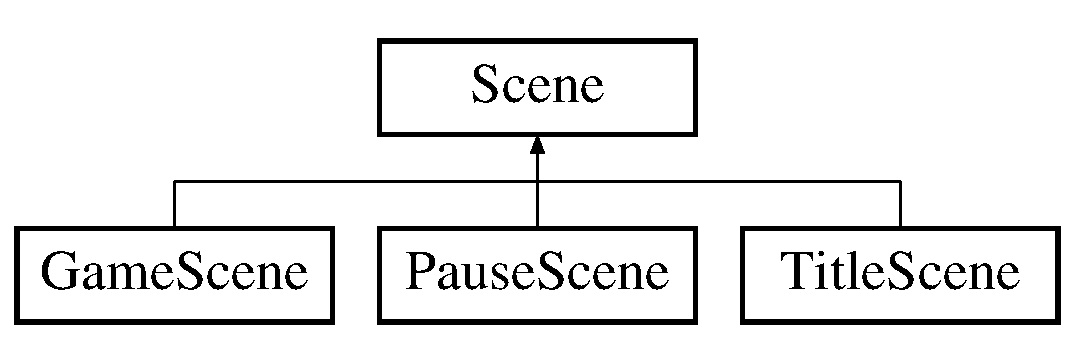
\includegraphics[height=2.000000cm]{class_scene}
\end{center}
\end{figure}
\subsection*{Classes}
\begin{DoxyCompactItemize}
\item 
struct \hyperlink{struct_scene_1_1_context}{Context}
\begin{DoxyCompactList}\small\item\em \hyperlink{struct_scene_1_1_context}{Context} holds map to all textures, render window and all fonts. Only one instance is every created and passed around. \end{DoxyCompactList}\end{DoxyCompactItemize}
\subsection*{Public Member Functions}
\begin{DoxyCompactItemize}
\item 
\hyperlink{class_scene_a9834819a1140a2c066024927e6dc9692}{Scene} (\hyperlink{class_scene_stack}{Scene\+Stack} \&stack, \hyperlink{struct_scene_1_1_context}{Context} context)
\item 
virtual \hyperlink{class_scene_a3b8cec2e32546713915f8c6303c951f1}{$\sim$\+Scene} ()
\item 
virtual void \hyperlink{class_scene_a789c16961aa1e316b2a4a05b95187546}{draw} ()=0
\item 
virtual bool \hyperlink{class_scene_a72683c984a1da2ce4f757705e93730f2}{update} (sf\+::\+Time delta\+Time)=0
\item 
virtual bool \hyperlink{class_scene_af25e4d2c998aca4e95899fb67488e815}{handle\+Event} (const sf\+::\+Event \&event)=0
\end{DoxyCompactItemize}
\subsection*{Protected Member Functions}
\begin{DoxyCompactItemize}
\item 
void \hyperlink{class_scene_a38d36125a421eab649188edb740d1c36}{request\+Stack\+Push} (\hyperlink{namespace_scenes_a0ad7ab6856b1d77d498e3a251f6bb275}{Scenes\+::\+ID} scene\+ID)
\item 
void \hyperlink{class_scene_ad2f2093a8adc09c11e89cda6f94a3dd1}{request\+Stack\+Pop} ()
\item 
void \hyperlink{class_scene_a0cc91a92f27ba281b52c58168b7a000a}{request\+State\+Clear} ()
\item 
\hyperlink{struct_scene_1_1_context}{Context} \hyperlink{class_scene_acab4ecf24b21ffa8e423a8e4fd45c491}{get\+Context} () const
\end{DoxyCompactItemize}


\subsection{Constructor \& Destructor Documentation}
\mbox{\Hypertarget{class_scene_a9834819a1140a2c066024927e6dc9692}\label{class_scene_a9834819a1140a2c066024927e6dc9692}} 
\index{Scene@{Scene}!Scene@{Scene}}
\index{Scene@{Scene}!Scene@{Scene}}
\subsubsection{\texorpdfstring{Scene()}{Scene()}}
{\footnotesize\ttfamily Scene\+::\+Scene (\begin{DoxyParamCaption}\item[{\hyperlink{class_scene_stack}{Scene\+Stack} \&}]{stack,  }\item[{\hyperlink{struct_scene_1_1_context}{Context}}]{context }\end{DoxyParamCaption})}

\mbox{\Hypertarget{class_scene_a3b8cec2e32546713915f8c6303c951f1}\label{class_scene_a3b8cec2e32546713915f8c6303c951f1}} 
\index{Scene@{Scene}!````~Scene@{$\sim$\+Scene}}
\index{````~Scene@{$\sim$\+Scene}!Scene@{Scene}}
\subsubsection{\texorpdfstring{$\sim$\+Scene()}{~Scene()}}
{\footnotesize\ttfamily Scene\+::$\sim$\+Scene (\begin{DoxyParamCaption}{ }\end{DoxyParamCaption})\hspace{0.3cm}{\ttfamily [virtual]}}



\subsection{Member Function Documentation}
\mbox{\Hypertarget{class_scene_a789c16961aa1e316b2a4a05b95187546}\label{class_scene_a789c16961aa1e316b2a4a05b95187546}} 
\index{Scene@{Scene}!draw@{draw}}
\index{draw@{draw}!Scene@{Scene}}
\subsubsection{\texorpdfstring{draw()}{draw()}}
{\footnotesize\ttfamily virtual void Scene\+::draw (\begin{DoxyParamCaption}{ }\end{DoxyParamCaption})\hspace{0.3cm}{\ttfamily [pure virtual]}}

\hyperlink{class_scene}{Scene} virtual draw function 

Implemented in \hyperlink{class_game_scene_ae9eb60cbb8fa55eeb07b951e3d83f426}{Game\+Scene}, \hyperlink{class_gameover_scene_ae8a5e79e002d0e79edaec9ec1b0df902}{Gameover\+Scene}, \hyperlink{class_pause_scene_abfd1398a064a83b3ae6ac5fd98aebf05}{Pause\+Scene}, and \hyperlink{class_title_scene_a3e527255771f75a41c4fe8aaa35999dd}{Title\+Scene}.

\mbox{\Hypertarget{class_scene_acab4ecf24b21ffa8e423a8e4fd45c491}\label{class_scene_acab4ecf24b21ffa8e423a8e4fd45c491}} 
\index{Scene@{Scene}!get\+Context@{get\+Context}}
\index{get\+Context@{get\+Context}!Scene@{Scene}}
\subsubsection{\texorpdfstring{get\+Context()}{getContext()}}
{\footnotesize\ttfamily \hyperlink{struct_scene_1_1_context}{Scene\+::\+Context} Scene\+::get\+Context (\begin{DoxyParamCaption}{ }\end{DoxyParamCaption}) const\hspace{0.3cm}{\ttfamily [protected]}}

Returns context \mbox{\Hypertarget{class_scene_af25e4d2c998aca4e95899fb67488e815}\label{class_scene_af25e4d2c998aca4e95899fb67488e815}} 
\index{Scene@{Scene}!handle\+Event@{handle\+Event}}
\index{handle\+Event@{handle\+Event}!Scene@{Scene}}
\subsubsection{\texorpdfstring{handle\+Event()}{handleEvent()}}
{\footnotesize\ttfamily virtual bool Scene\+::handle\+Event (\begin{DoxyParamCaption}\item[{const sf\+::\+Event \&}]{event }\end{DoxyParamCaption})\hspace{0.3cm}{\ttfamily [pure virtual]}}

\hyperlink{class_scene}{Scene} virtual handle event function 

Implemented in \hyperlink{class_game_scene_aa494372b1f451f3c3a268558fddb30f2}{Game\+Scene}, \hyperlink{class_gameover_scene_ac951bc51d29e2d14807e3da2e885ccc8}{Gameover\+Scene}, \hyperlink{class_pause_scene_adeb06e37e0a2afa297ddbe795c3cbe94}{Pause\+Scene}, and \hyperlink{class_title_scene_a1f019a83309ce967883b4b4d76b816af}{Title\+Scene}.

\mbox{\Hypertarget{class_scene_ad2f2093a8adc09c11e89cda6f94a3dd1}\label{class_scene_ad2f2093a8adc09c11e89cda6f94a3dd1}} 
\index{Scene@{Scene}!request\+Stack\+Pop@{request\+Stack\+Pop}}
\index{request\+Stack\+Pop@{request\+Stack\+Pop}!Scene@{Scene}}
\subsubsection{\texorpdfstring{request\+Stack\+Pop()}{requestStackPop()}}
{\footnotesize\ttfamily void Scene\+::request\+Stack\+Pop (\begin{DoxyParamCaption}{ }\end{DoxyParamCaption})\hspace{0.3cm}{\ttfamily [protected]}}

Request scene to be popped \mbox{\Hypertarget{class_scene_a38d36125a421eab649188edb740d1c36}\label{class_scene_a38d36125a421eab649188edb740d1c36}} 
\index{Scene@{Scene}!request\+Stack\+Push@{request\+Stack\+Push}}
\index{request\+Stack\+Push@{request\+Stack\+Push}!Scene@{Scene}}
\subsubsection{\texorpdfstring{request\+Stack\+Push()}{requestStackPush()}}
{\footnotesize\ttfamily void Scene\+::request\+Stack\+Push (\begin{DoxyParamCaption}\item[{\hyperlink{namespace_scenes_a0ad7ab6856b1d77d498e3a251f6bb275}{Scenes\+::\+ID}}]{scene\+ID }\end{DoxyParamCaption})\hspace{0.3cm}{\ttfamily [protected]}}

Request scene to be pushed \mbox{\Hypertarget{class_scene_a0cc91a92f27ba281b52c58168b7a000a}\label{class_scene_a0cc91a92f27ba281b52c58168b7a000a}} 
\index{Scene@{Scene}!request\+State\+Clear@{request\+State\+Clear}}
\index{request\+State\+Clear@{request\+State\+Clear}!Scene@{Scene}}
\subsubsection{\texorpdfstring{request\+State\+Clear()}{requestStateClear()}}
{\footnotesize\ttfamily void Scene\+::request\+State\+Clear (\begin{DoxyParamCaption}{ }\end{DoxyParamCaption})\hspace{0.3cm}{\ttfamily [protected]}}

Request Flushing the stack of scenes \mbox{\Hypertarget{class_scene_a72683c984a1da2ce4f757705e93730f2}\label{class_scene_a72683c984a1da2ce4f757705e93730f2}} 
\index{Scene@{Scene}!update@{update}}
\index{update@{update}!Scene@{Scene}}
\subsubsection{\texorpdfstring{update()}{update()}}
{\footnotesize\ttfamily virtual bool Scene\+::update (\begin{DoxyParamCaption}\item[{sf\+::\+Time}]{delta\+Time }\end{DoxyParamCaption})\hspace{0.3cm}{\ttfamily [pure virtual]}}

\hyperlink{class_scene}{Scene} virtual update function 

Implemented in \hyperlink{class_game_scene_ae54628d2f041bcad66242584b2db10d6}{Game\+Scene}, \hyperlink{class_gameover_scene_a6b7f650af840f54c78b4fb1cdf2010df}{Gameover\+Scene}, \hyperlink{class_pause_scene_a8504260009b4dfb2380785e938e60b4b}{Pause\+Scene}, and \hyperlink{class_title_scene_a17ce1b5b9f6f8ca44a6ed3326e9e5d0a}{Title\+Scene}.



The documentation for this class was generated from the following files\+:\begin{DoxyCompactItemize}
\item 
S\+F\+M\+L Engine/\hyperlink{_scene_8h}{Scene.\+h}\item 
S\+F\+M\+L Engine/\hyperlink{_scene_8cpp}{Scene.\+cpp}\end{DoxyCompactItemize}

\hypertarget{class_scene_stack}{}\section{Scene\+Stack Class Reference}
\label{class_scene_stack}\index{Scene\+Stack@{Scene\+Stack}}


Controls the changing of scenes.  




{\ttfamily \#include $<$Scene\+Stack.\+h$>$}

Inheritance diagram for Scene\+Stack\+:\begin{figure}[H]
\begin{center}
\leavevmode
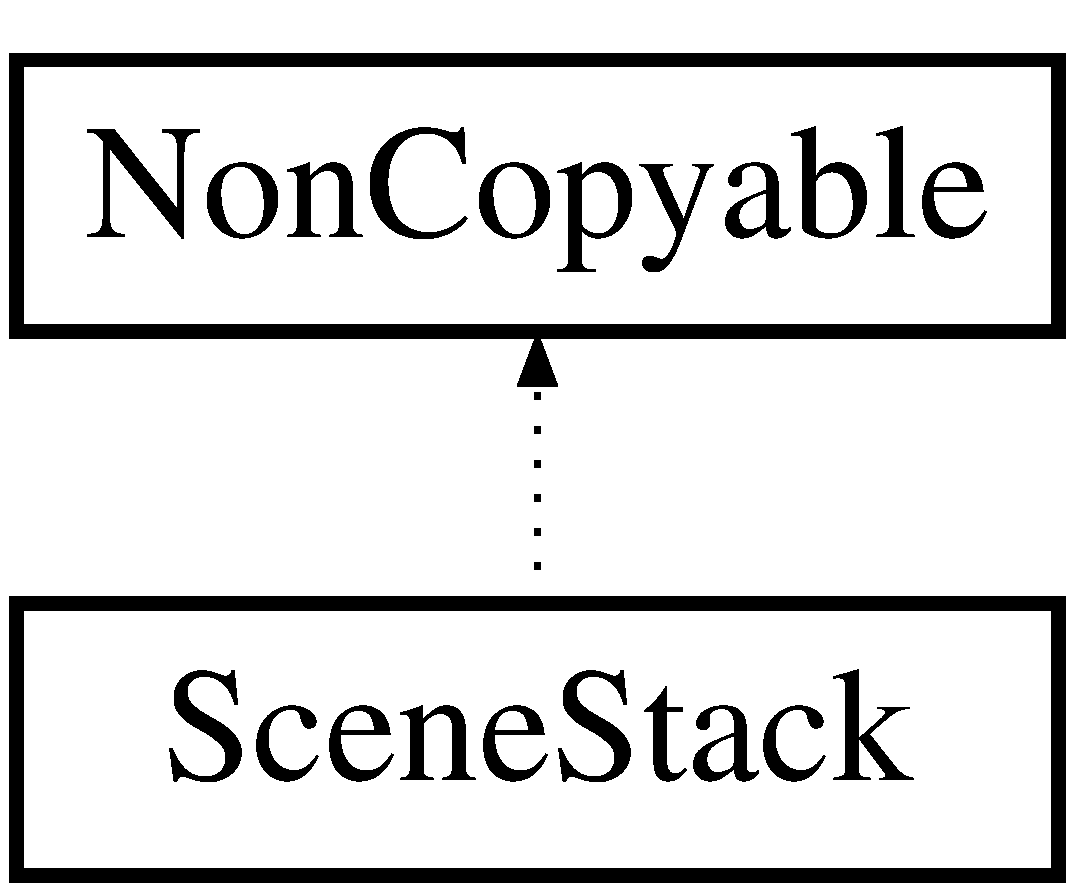
\includegraphics[height=2.000000cm]{class_scene_stack}
\end{center}
\end{figure}
\subsection*{Public Types}
\begin{DoxyCompactItemize}
\item 
enum \hyperlink{class_scene_stack_ab8644e038aad992c6776dc3fb5fcc1f9}{Action} \{ \hyperlink{class_scene_stack_ab8644e038aad992c6776dc3fb5fcc1f9a6cd7480d27e0a88a4b67e2186757358d}{Push}, 
\hyperlink{class_scene_stack_ab8644e038aad992c6776dc3fb5fcc1f9a1d86b0e7cf0989e5717f70598e74fa95}{Pop}, 
\hyperlink{class_scene_stack_ab8644e038aad992c6776dc3fb5fcc1f9af03df5d6746e57023c22bb3548b93779}{Clear}
 \}
\end{DoxyCompactItemize}
\subsection*{Public Member Functions}
\begin{DoxyCompactItemize}
\item 
\hyperlink{class_scene_stack_a7893580d1266ed06c9c690012137f799}{Scene\+Stack} (\hyperlink{struct_scene_1_1_context}{Scene\+::\+Context} context)
\item 
{\footnotesize template$<$typename T $>$ }\\void \hyperlink{class_scene_stack_a129b49c7bc280aeaf7c71235b3d9648d}{create\+Scene} (\hyperlink{namespace_scenes_a0ad7ab6856b1d77d498e3a251f6bb275}{Scenes\+::\+ID} scene\+ID)
\item 
void \hyperlink{class_scene_stack_acdea2588bbc85c2834608ebab6671866}{update} (sf\+::\+Time delta\+Time)
\item 
void \hyperlink{class_scene_stack_ab4a68b2247289ba1d934067aad35159d}{draw} ()
\item 
void \hyperlink{class_scene_stack_aecf75add55f527c31528043f4b28db44}{handle\+Event} (const sf\+::\+Event \&event)
\item 
void \hyperlink{class_scene_stack_a41366819a998558e3920fe7859d1f114}{push\+Scene} (\hyperlink{namespace_scenes_a0ad7ab6856b1d77d498e3a251f6bb275}{Scenes\+::\+ID} scene\+ID)
\item 
void \hyperlink{class_scene_stack_a0ea3309f9ec9120cf51a0bce3881e1e2}{pop\+Scene} ()
\item 
void \hyperlink{class_scene_stack_a70253c72c07f5d5c5d77861d064b8470}{clear\+Scene} ()
\item 
bool \hyperlink{class_scene_stack_ade95cce69229a18d169f63093289e865}{is\+Empty} () const
\end{DoxyCompactItemize}


\subsection{Detailed Description}
Controls the changing of scenes. 



\subsection{Member Enumeration Documentation}
\mbox{\Hypertarget{class_scene_stack_ab8644e038aad992c6776dc3fb5fcc1f9}\label{class_scene_stack_ab8644e038aad992c6776dc3fb5fcc1f9}} 
\index{Scene\+Stack@{Scene\+Stack}!Action@{Action}}
\index{Action@{Action}!Scene\+Stack@{Scene\+Stack}}
\subsubsection{\texorpdfstring{Action}{Action}}
{\footnotesize\ttfamily enum \hyperlink{class_scene_stack_ab8644e038aad992c6776dc3fb5fcc1f9}{Scene\+Stack\+::\+Action}}

\begin{DoxyEnumFields}{Enumerator}
\raisebox{\heightof{T}}[0pt][0pt]{\index{Push@{Push}!Scene\+Stack@{Scene\+Stack}}\index{Scene\+Stack@{Scene\+Stack}!Push@{Push}}}\mbox{\Hypertarget{class_scene_stack_ab8644e038aad992c6776dc3fb5fcc1f9a6cd7480d27e0a88a4b67e2186757358d}\label{class_scene_stack_ab8644e038aad992c6776dc3fb5fcc1f9a6cd7480d27e0a88a4b67e2186757358d}} 
Push&\\
\hline

\raisebox{\heightof{T}}[0pt][0pt]{\index{Pop@{Pop}!Scene\+Stack@{Scene\+Stack}}\index{Scene\+Stack@{Scene\+Stack}!Pop@{Pop}}}\mbox{\Hypertarget{class_scene_stack_ab8644e038aad992c6776dc3fb5fcc1f9a1d86b0e7cf0989e5717f70598e74fa95}\label{class_scene_stack_ab8644e038aad992c6776dc3fb5fcc1f9a1d86b0e7cf0989e5717f70598e74fa95}} 
Pop&\\
\hline

\raisebox{\heightof{T}}[0pt][0pt]{\index{Clear@{Clear}!Scene\+Stack@{Scene\+Stack}}\index{Scene\+Stack@{Scene\+Stack}!Clear@{Clear}}}\mbox{\Hypertarget{class_scene_stack_ab8644e038aad992c6776dc3fb5fcc1f9af03df5d6746e57023c22bb3548b93779}\label{class_scene_stack_ab8644e038aad992c6776dc3fb5fcc1f9af03df5d6746e57023c22bb3548b93779}} 
Clear&\\
\hline

\end{DoxyEnumFields}


\subsection{Constructor \& Destructor Documentation}
\mbox{\Hypertarget{class_scene_stack_a7893580d1266ed06c9c690012137f799}\label{class_scene_stack_a7893580d1266ed06c9c690012137f799}} 
\index{Scene\+Stack@{Scene\+Stack}!Scene\+Stack@{Scene\+Stack}}
\index{Scene\+Stack@{Scene\+Stack}!Scene\+Stack@{Scene\+Stack}}
\subsubsection{\texorpdfstring{Scene\+Stack()}{SceneStack()}}
{\footnotesize\ttfamily Scene\+Stack\+::\+Scene\+Stack (\begin{DoxyParamCaption}\item[{\hyperlink{struct_scene_1_1_context}{Scene\+::\+Context}}]{context }\end{DoxyParamCaption})\hspace{0.3cm}{\ttfamily [explicit]}}



\subsection{Member Function Documentation}
\mbox{\Hypertarget{class_scene_stack_a70253c72c07f5d5c5d77861d064b8470}\label{class_scene_stack_a70253c72c07f5d5c5d77861d064b8470}} 
\index{Scene\+Stack@{Scene\+Stack}!clear\+Scene@{clear\+Scene}}
\index{clear\+Scene@{clear\+Scene}!Scene\+Stack@{Scene\+Stack}}
\subsubsection{\texorpdfstring{clear\+Scene()}{clearScene()}}
{\footnotesize\ttfamily void Scene\+Stack\+::clear\+Scene (\begin{DoxyParamCaption}{ }\end{DoxyParamCaption})}

\mbox{\Hypertarget{class_scene_stack_a129b49c7bc280aeaf7c71235b3d9648d}\label{class_scene_stack_a129b49c7bc280aeaf7c71235b3d9648d}} 
\index{Scene\+Stack@{Scene\+Stack}!create\+Scene@{create\+Scene}}
\index{create\+Scene@{create\+Scene}!Scene\+Stack@{Scene\+Stack}}
\subsubsection{\texorpdfstring{create\+Scene()}{createScene()}}
{\footnotesize\ttfamily template$<$typename T $>$ \\
void Scene\+Stack\+::create\+Scene (\begin{DoxyParamCaption}\item[{\hyperlink{namespace_scenes_a0ad7ab6856b1d77d498e3a251f6bb275}{Scenes\+::\+ID}}]{scene\+ID }\end{DoxyParamCaption})}

\mbox{\Hypertarget{class_scene_stack_ab4a68b2247289ba1d934067aad35159d}\label{class_scene_stack_ab4a68b2247289ba1d934067aad35159d}} 
\index{Scene\+Stack@{Scene\+Stack}!draw@{draw}}
\index{draw@{draw}!Scene\+Stack@{Scene\+Stack}}
\subsubsection{\texorpdfstring{draw()}{draw()}}
{\footnotesize\ttfamily void Scene\+Stack\+::draw (\begin{DoxyParamCaption}{ }\end{DoxyParamCaption})}

\mbox{\Hypertarget{class_scene_stack_aecf75add55f527c31528043f4b28db44}\label{class_scene_stack_aecf75add55f527c31528043f4b28db44}} 
\index{Scene\+Stack@{Scene\+Stack}!handle\+Event@{handle\+Event}}
\index{handle\+Event@{handle\+Event}!Scene\+Stack@{Scene\+Stack}}
\subsubsection{\texorpdfstring{handle\+Event()}{handleEvent()}}
{\footnotesize\ttfamily void Scene\+Stack\+::handle\+Event (\begin{DoxyParamCaption}\item[{const sf\+::\+Event \&}]{event }\end{DoxyParamCaption})}

\mbox{\Hypertarget{class_scene_stack_ade95cce69229a18d169f63093289e865}\label{class_scene_stack_ade95cce69229a18d169f63093289e865}} 
\index{Scene\+Stack@{Scene\+Stack}!is\+Empty@{is\+Empty}}
\index{is\+Empty@{is\+Empty}!Scene\+Stack@{Scene\+Stack}}
\subsubsection{\texorpdfstring{is\+Empty()}{isEmpty()}}
{\footnotesize\ttfamily bool Scene\+Stack\+::is\+Empty (\begin{DoxyParamCaption}{ }\end{DoxyParamCaption}) const}

\mbox{\Hypertarget{class_scene_stack_a0ea3309f9ec9120cf51a0bce3881e1e2}\label{class_scene_stack_a0ea3309f9ec9120cf51a0bce3881e1e2}} 
\index{Scene\+Stack@{Scene\+Stack}!pop\+Scene@{pop\+Scene}}
\index{pop\+Scene@{pop\+Scene}!Scene\+Stack@{Scene\+Stack}}
\subsubsection{\texorpdfstring{pop\+Scene()}{popScene()}}
{\footnotesize\ttfamily void Scene\+Stack\+::pop\+Scene (\begin{DoxyParamCaption}{ }\end{DoxyParamCaption})}

\mbox{\Hypertarget{class_scene_stack_a41366819a998558e3920fe7859d1f114}\label{class_scene_stack_a41366819a998558e3920fe7859d1f114}} 
\index{Scene\+Stack@{Scene\+Stack}!push\+Scene@{push\+Scene}}
\index{push\+Scene@{push\+Scene}!Scene\+Stack@{Scene\+Stack}}
\subsubsection{\texorpdfstring{push\+Scene()}{pushScene()}}
{\footnotesize\ttfamily void Scene\+Stack\+::push\+Scene (\begin{DoxyParamCaption}\item[{\hyperlink{namespace_scenes_a0ad7ab6856b1d77d498e3a251f6bb275}{Scenes\+::\+ID}}]{scene\+ID }\end{DoxyParamCaption})}

\mbox{\Hypertarget{class_scene_stack_acdea2588bbc85c2834608ebab6671866}\label{class_scene_stack_acdea2588bbc85c2834608ebab6671866}} 
\index{Scene\+Stack@{Scene\+Stack}!update@{update}}
\index{update@{update}!Scene\+Stack@{Scene\+Stack}}
\subsubsection{\texorpdfstring{update()}{update()}}
{\footnotesize\ttfamily void Scene\+Stack\+::update (\begin{DoxyParamCaption}\item[{sf\+::\+Time}]{delta\+Time }\end{DoxyParamCaption})}



The documentation for this class was generated from the following files\+:\begin{DoxyCompactItemize}
\item 
S\+F\+M\+L Engine/\hyperlink{_scene_stack_8h}{Scene\+Stack.\+h}\item 
S\+F\+M\+L Engine/\hyperlink{_scene_stack_8cpp}{Scene\+Stack.\+cpp}\end{DoxyCompactItemize}

\hypertarget{class_sound_player}{}\section{Sound\+Player Class Reference}
\label{class_sound_player}\index{Sound\+Player@{Sound\+Player}}


{\ttfamily \#include $<$Sound\+Player.\+h$>$}

\subsection*{Public Member Functions}
\begin{DoxyCompactItemize}
\item 
void \hyperlink{class_sound_player_aa0b85f15f5b13bc41c71eeee6b0a7779}{play} (\hyperlink{namespace_sound_effect_a11ffbf1eb89e85a34cbfd5a59b2cd9cb}{Sound\+Effect\+::\+ID} effect)
\item 
void \hyperlink{class_sound_player_a3fd165dadf60b580b16367b81d84681b}{remove\+Stopped\+Sounds} ()
\end{DoxyCompactItemize}
\subsection*{Static Public Member Functions}
\begin{DoxyCompactItemize}
\item 
static \hyperlink{class_sound_player}{Sound\+Player} $\ast$ \hyperlink{class_sound_player_a4458c33c6054f60a9cd70cdbb2d1cdb0}{Instance} ()
\end{DoxyCompactItemize}


\subsection{Member Function Documentation}
\mbox{\Hypertarget{class_sound_player_a4458c33c6054f60a9cd70cdbb2d1cdb0}\label{class_sound_player_a4458c33c6054f60a9cd70cdbb2d1cdb0}} 
\index{Sound\+Player@{Sound\+Player}!Instance@{Instance}}
\index{Instance@{Instance}!Sound\+Player@{Sound\+Player}}
\subsubsection{\texorpdfstring{Instance()}{Instance()}}
{\footnotesize\ttfamily \hyperlink{class_sound_player}{Sound\+Player} $\ast$ Sound\+Player\+::\+Instance (\begin{DoxyParamCaption}{ }\end{DoxyParamCaption})\hspace{0.3cm}{\ttfamily [static]}}

\mbox{\Hypertarget{class_sound_player_aa0b85f15f5b13bc41c71eeee6b0a7779}\label{class_sound_player_aa0b85f15f5b13bc41c71eeee6b0a7779}} 
\index{Sound\+Player@{Sound\+Player}!play@{play}}
\index{play@{play}!Sound\+Player@{Sound\+Player}}
\subsubsection{\texorpdfstring{play()}{play()}}
{\footnotesize\ttfamily void Sound\+Player\+::play (\begin{DoxyParamCaption}\item[{\hyperlink{namespace_sound_effect_a11ffbf1eb89e85a34cbfd5a59b2cd9cb}{Sound\+Effect\+::\+ID}}]{effect }\end{DoxyParamCaption})}

\mbox{\Hypertarget{class_sound_player_a3fd165dadf60b580b16367b81d84681b}\label{class_sound_player_a3fd165dadf60b580b16367b81d84681b}} 
\index{Sound\+Player@{Sound\+Player}!remove\+Stopped\+Sounds@{remove\+Stopped\+Sounds}}
\index{remove\+Stopped\+Sounds@{remove\+Stopped\+Sounds}!Sound\+Player@{Sound\+Player}}
\subsubsection{\texorpdfstring{remove\+Stopped\+Sounds()}{removeStoppedSounds()}}
{\footnotesize\ttfamily void Sound\+Player\+::remove\+Stopped\+Sounds (\begin{DoxyParamCaption}{ }\end{DoxyParamCaption})}



The documentation for this class was generated from the following files\+:\begin{DoxyCompactItemize}
\item 
S\+F\+M\+L Engine/\hyperlink{_sound_player_8h}{Sound\+Player.\+h}\item 
S\+F\+M\+L Engine/\hyperlink{_sound_player_8cpp}{Sound\+Player.\+cpp}\end{DoxyCompactItemize}

\hypertarget{class_title_scene}{}\section{Title\+Scene Class Reference}
\label{class_title_scene}\index{Title\+Scene@{Title\+Scene}}


{\ttfamily \#include $<$Title\+Scene.\+h$>$}

Inheritance diagram for Title\+Scene\+:\begin{figure}[H]
\begin{center}
\leavevmode
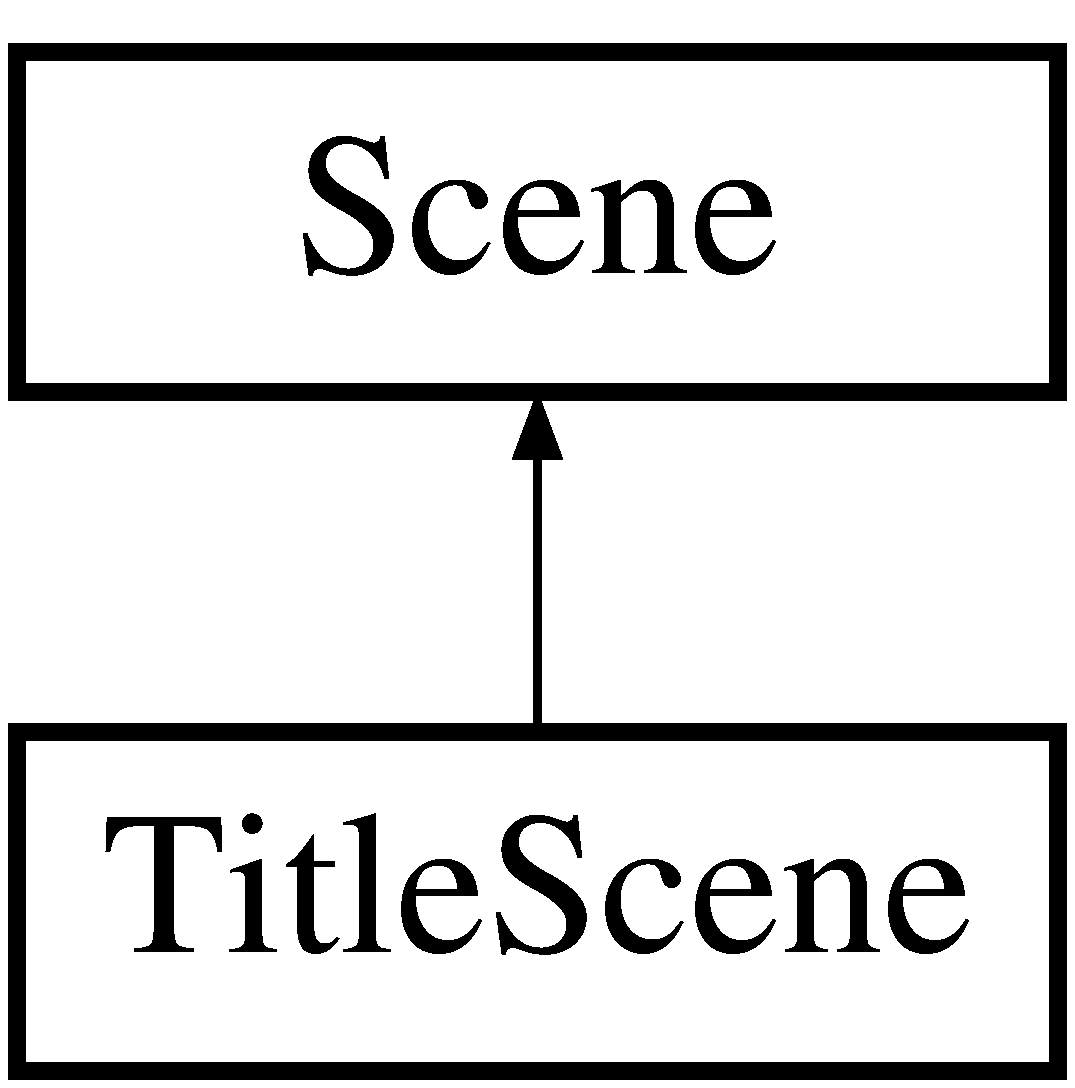
\includegraphics[height=2.000000cm]{class_title_scene}
\end{center}
\end{figure}
\subsection*{Public Member Functions}
\begin{DoxyCompactItemize}
\item 
\hyperlink{class_title_scene_a280a3b1e5890f45b932860777f8fbe6d}{Title\+Scene} (\hyperlink{class_scene_stack}{Scene\+Stack} \&stack, \hyperlink{struct_scene_1_1_context}{Context} context)
\item 
void \hyperlink{class_title_scene_a3e527255771f75a41c4fe8aaa35999dd}{draw} () override
\item 
bool \hyperlink{class_title_scene_a17ce1b5b9f6f8ca44a6ed3326e9e5d0a}{update} (sf\+::\+Time delta\+Time) override
\item 
bool \hyperlink{class_title_scene_a1f019a83309ce967883b4b4d76b816af}{handle\+Event} (const sf\+::\+Event \&event) override
\end{DoxyCompactItemize}
\subsection*{Additional Inherited Members}


\subsection{Constructor \& Destructor Documentation}
\mbox{\Hypertarget{class_title_scene_a280a3b1e5890f45b932860777f8fbe6d}\label{class_title_scene_a280a3b1e5890f45b932860777f8fbe6d}} 
\index{Title\+Scene@{Title\+Scene}!Title\+Scene@{Title\+Scene}}
\index{Title\+Scene@{Title\+Scene}!Title\+Scene@{Title\+Scene}}
\subsubsection{\texorpdfstring{Title\+Scene()}{TitleScene()}}
{\footnotesize\ttfamily Title\+Scene\+::\+Title\+Scene (\begin{DoxyParamCaption}\item[{\hyperlink{class_scene_stack}{Scene\+Stack} \&}]{stack,  }\item[{\hyperlink{struct_scene_1_1_context}{Context}}]{context }\end{DoxyParamCaption})}



\subsection{Member Function Documentation}
\mbox{\Hypertarget{class_title_scene_a3e527255771f75a41c4fe8aaa35999dd}\label{class_title_scene_a3e527255771f75a41c4fe8aaa35999dd}} 
\index{Title\+Scene@{Title\+Scene}!draw@{draw}}
\index{draw@{draw}!Title\+Scene@{Title\+Scene}}
\subsubsection{\texorpdfstring{draw()}{draw()}}
{\footnotesize\ttfamily void Title\+Scene\+::draw (\begin{DoxyParamCaption}{ }\end{DoxyParamCaption})\hspace{0.3cm}{\ttfamily [override]}, {\ttfamily [virtual]}}



Implements \hyperlink{class_scene_a789c16961aa1e316b2a4a05b95187546}{Scene}.

\mbox{\Hypertarget{class_title_scene_a1f019a83309ce967883b4b4d76b816af}\label{class_title_scene_a1f019a83309ce967883b4b4d76b816af}} 
\index{Title\+Scene@{Title\+Scene}!handle\+Event@{handle\+Event}}
\index{handle\+Event@{handle\+Event}!Title\+Scene@{Title\+Scene}}
\subsubsection{\texorpdfstring{handle\+Event()}{handleEvent()}}
{\footnotesize\ttfamily bool Title\+Scene\+::handle\+Event (\begin{DoxyParamCaption}\item[{const sf\+::\+Event \&}]{event }\end{DoxyParamCaption})\hspace{0.3cm}{\ttfamily [override]}, {\ttfamily [virtual]}}



Implements \hyperlink{class_scene_af25e4d2c998aca4e95899fb67488e815}{Scene}.

\mbox{\Hypertarget{class_title_scene_a17ce1b5b9f6f8ca44a6ed3326e9e5d0a}\label{class_title_scene_a17ce1b5b9f6f8ca44a6ed3326e9e5d0a}} 
\index{Title\+Scene@{Title\+Scene}!update@{update}}
\index{update@{update}!Title\+Scene@{Title\+Scene}}
\subsubsection{\texorpdfstring{update()}{update()}}
{\footnotesize\ttfamily bool Title\+Scene\+::update (\begin{DoxyParamCaption}\item[{sf\+::\+Time}]{delta\+Time }\end{DoxyParamCaption})\hspace{0.3cm}{\ttfamily [override]}, {\ttfamily [virtual]}}



Implements \hyperlink{class_scene_a72683c984a1da2ce4f757705e93730f2}{Scene}.



The documentation for this class was generated from the following files\+:\begin{DoxyCompactItemize}
\item 
S\+F\+M\+L Engine/\hyperlink{_title_scene_8h}{Title\+Scene.\+h}\item 
S\+F\+M\+L Engine/\hyperlink{_title_scene_8cpp}{Title\+Scene.\+cpp}\end{DoxyCompactItemize}

\chapter{File Documentation}
\hypertarget{_animated_sprite_8cpp}{}\section{S\+F\+ML Engine/\+Animated\+Sprite.cpp File Reference}
\label{_animated_sprite_8cpp}\index{S\+F\+M\+L Engine/\+Animated\+Sprite.\+cpp@{S\+F\+M\+L Engine/\+Animated\+Sprite.\+cpp}}
{\ttfamily \#include \char`\"{}stdafx.\+h\char`\"{}}\newline
{\ttfamily \#include \char`\"{}Animated\+Sprite.\+h\char`\"{}}\newline

\hypertarget{_animated_sprite_8h}{}\section{S\+F\+ML Engine/\+S\+F\+ML Engine/\+Animated\+Sprite.h File Reference}
\label{_animated_sprite_8h}\index{S\+F\+M\+L Engine/\+S\+F\+M\+L Engine/\+Animated\+Sprite.\+h@{S\+F\+M\+L Engine/\+S\+F\+M\+L Engine/\+Animated\+Sprite.\+h}}
{\ttfamily \#include $<$S\+F\+M\+L/\+Graphics/\+Render\+Target.\+hpp$>$}\newline
{\ttfamily \#include $<$S\+F\+M\+L/\+System/\+Time.\+hpp$>$}\newline
{\ttfamily \#include $<$S\+F\+M\+L/\+Graphics/\+Drawable.\+hpp$>$}\newline
{\ttfamily \#include $<$S\+F\+M\+L/\+Graphics/\+Transformable.\+hpp$>$}\newline
{\ttfamily \#include $<$S\+F\+M\+L/\+System/\+Vector2.\+hpp$>$}\newline
{\ttfamily \#include \char`\"{}Animation.\+h\char`\"{}}\newline
{\ttfamily \#include \char`\"{}Animated\+Sprite.\+h\char`\"{}}\newline
\subsection*{Classes}
\begin{DoxyCompactItemize}
\item 
class \hyperlink{class_animated_sprite}{Animated\+Sprite}
\end{DoxyCompactItemize}

\hypertarget{_animation_8cpp}{}\section{S\+F\+ML Engine/\+S\+F\+ML Engine/\+Animation.cpp File Reference}
\label{_animation_8cpp}\index{S\+F\+M\+L Engine/\+S\+F\+M\+L Engine/\+Animation.\+cpp@{S\+F\+M\+L Engine/\+S\+F\+M\+L Engine/\+Animation.\+cpp}}
{\ttfamily \#include \char`\"{}stdafx.\+h\char`\"{}}\newline
{\ttfamily \#include \char`\"{}Animation.\+h\char`\"{}}\newline

\hypertarget{_animation_8h}{}\section{S\+F\+ML Engine/\+S\+F\+ML Engine/\+Animation.h File Reference}
\label{_animation_8h}\index{S\+F\+M\+L Engine/\+S\+F\+M\+L Engine/\+Animation.\+h@{S\+F\+M\+L Engine/\+S\+F\+M\+L Engine/\+Animation.\+h}}
{\ttfamily \#include $<$vector$>$}\newline
{\ttfamily \#include $<$S\+F\+M\+L/\+Graphics/\+Rect.\+hpp$>$}\newline
{\ttfamily \#include $<$S\+F\+M\+L/\+Graphics/\+Texture.\+hpp$>$}\newline
\subsection*{Classes}
\begin{DoxyCompactItemize}
\item 
class \hyperlink{class_animation}{Animation}
\end{DoxyCompactItemize}

\hypertarget{_application_8cpp}{}\section{S\+F\+ML Engine/\+Application.cpp File Reference}
\label{_application_8cpp}\index{S\+F\+M\+L Engine/\+Application.\+cpp@{S\+F\+M\+L Engine/\+Application.\+cpp}}
{\ttfamily \#include \char`\"{}stdafx.\+h\char`\"{}}\newline
{\ttfamily \#include \char`\"{}Application.\+h\char`\"{}}\newline
{\ttfamily \#include \char`\"{}Scene.\+h\char`\"{}}\newline
{\ttfamily \#include \char`\"{}Title\+Scene.\+h\char`\"{}}\newline
{\ttfamily \#include \char`\"{}Game\+Scene.\+h\char`\"{}}\newline
{\ttfamily \#include \char`\"{}Pause\+Scene.\+h\char`\"{}}\newline
{\ttfamily \#include \char`\"{}Gameover\+Scene.\+h\char`\"{}}\newline
{\ttfamily \#include \char`\"{}Scene\+Identifiers.\+h\char`\"{}}\newline

\hypertarget{_application_8h}{}\section{S\+F\+ML Engine/\+Application.h File Reference}
\label{_application_8h}\index{S\+F\+M\+L Engine/\+Application.\+h@{S\+F\+M\+L Engine/\+Application.\+h}}
{\ttfamily \#include $<$S\+F\+M\+L/\+Graphics.\+hpp$>$}\newline
{\ttfamily \#include \char`\"{}Resource\+Holder.\+h\char`\"{}}\newline
{\ttfamily \#include \char`\"{}Scene\+Stack.\+h\char`\"{}}\newline
{\ttfamily \#include \char`\"{}Scene\+Identifiers.\+h\char`\"{}}\newline
{\ttfamily \#include \char`\"{}Sound\+Player.\+h\char`\"{}}\newline
\subsection*{Classes}
\begin{DoxyCompactItemize}
\item 
class \hyperlink{class_application}{Application}
\begin{DoxyCompactList}\small\item\em Handles the input, loading of textures and fonts, creates scenes. \end{DoxyCompactList}\end{DoxyCompactItemize}

\hypertarget{_astronaut_8cpp}{}\section{S\+F\+ML Engine/\+Astronaut.cpp File Reference}
\label{_astronaut_8cpp}\index{S\+F\+M\+L Engine/\+Astronaut.\+cpp@{S\+F\+M\+L Engine/\+Astronaut.\+cpp}}
{\ttfamily \#include \char`\"{}stdafx.\+h\char`\"{}}\newline
{\ttfamily \#include \char`\"{}Astronaut.\+h\char`\"{}}\newline

\hypertarget{_astronaut_8h}{}\section{S\+F\+ML Engine/\+S\+F\+ML Engine/\+Astronaut.h File Reference}
\label{_astronaut_8h}\index{S\+F\+M\+L Engine/\+S\+F\+M\+L Engine/\+Astronaut.\+h@{S\+F\+M\+L Engine/\+S\+F\+M\+L Engine/\+Astronaut.\+h}}
{\ttfamily \#include $<$S\+F\+M\+L\textbackslash{}\+Graphics.\+hpp$>$}\newline
{\ttfamily \#include \char`\"{}Animated\+Sprite.\+h\char`\"{}}\newline
\subsection*{Classes}
\begin{DoxyCompactItemize}
\item 
class \hyperlink{class_astronaut}{Astronaut}
\end{DoxyCompactItemize}

\hypertarget{_bullet_8cpp}{}\section{S\+F\+ML Engine/\+S\+F\+ML Engine/\+Bullet.cpp File Reference}
\label{_bullet_8cpp}\index{S\+F\+M\+L Engine/\+S\+F\+M\+L Engine/\+Bullet.\+cpp@{S\+F\+M\+L Engine/\+S\+F\+M\+L Engine/\+Bullet.\+cpp}}
{\ttfamily \#include \char`\"{}stdafx.\+h\char`\"{}}\newline
{\ttfamily \#include \char`\"{}Bullet.\+h\char`\"{}}\newline

\hypertarget{_bullet_8h}{}\section{S\+F\+ML Engine/\+S\+F\+ML Engine/\+Bullet.h File Reference}
\label{_bullet_8h}\index{S\+F\+M\+L Engine/\+S\+F\+M\+L Engine/\+Bullet.\+h@{S\+F\+M\+L Engine/\+S\+F\+M\+L Engine/\+Bullet.\+h}}
{\ttfamily \#include \char`\"{}Animated\+Sprite.\+h\char`\"{}}\newline
{\ttfamily \#include \char`\"{}Helper.\+h\char`\"{}}\newline
{\ttfamily \#include $<$S\+F\+M\+L\textbackslash{}\+Graphics.\+hpp$>$}\newline
\subsection*{Classes}
\begin{DoxyCompactItemize}
\item 
class \hyperlink{class_bullet}{Bullet}
\end{DoxyCompactItemize}

\hypertarget{_camera_8cpp}{}\section{S\+F\+ML Engine/\+Camera.cpp File Reference}
\label{_camera_8cpp}\index{S\+F\+M\+L Engine/\+Camera.\+cpp@{S\+F\+M\+L Engine/\+Camera.\+cpp}}
{\ttfamily \#include \char`\"{}stdafx.\+h\char`\"{}}\newline
{\ttfamily \#include \char`\"{}Camera.\+h\char`\"{}}\newline

\hypertarget{_camera_8h}{}\section{S\+F\+ML Engine/\+S\+F\+ML Engine/\+Camera.h File Reference}
\label{_camera_8h}\index{S\+F\+M\+L Engine/\+S\+F\+M\+L Engine/\+Camera.\+h@{S\+F\+M\+L Engine/\+S\+F\+M\+L Engine/\+Camera.\+h}}
{\ttfamily \#include $<$S\+F\+M\+L\textbackslash{}\+Graphics.\+hpp$>$}\newline
\subsection*{Classes}
\begin{DoxyCompactItemize}
\item 
class \hyperlink{class_camera}{Camera}
\end{DoxyCompactItemize}

\hypertarget{_game_scene_8cpp}{}\section{S\+F\+ML Engine/\+S\+F\+ML Engine/\+Game\+Scene.cpp File Reference}
\label{_game_scene_8cpp}\index{S\+F\+M\+L Engine/\+S\+F\+M\+L Engine/\+Game\+Scene.\+cpp@{S\+F\+M\+L Engine/\+S\+F\+M\+L Engine/\+Game\+Scene.\+cpp}}
{\ttfamily \#include \char`\"{}stdafx.\+h\char`\"{}}\newline
{\ttfamily \#include \char`\"{}Game\+Scene.\+h\char`\"{}}\newline
{\ttfamily \#include $<$iostream$>$}\newline

\hypertarget{_game_scene_8h}{}\section{S\+F\+ML Engine/\+Game\+Scene.h File Reference}
\label{_game_scene_8h}\index{S\+F\+M\+L Engine/\+Game\+Scene.\+h@{S\+F\+M\+L Engine/\+Game\+Scene.\+h}}
{\ttfamily \#include \char`\"{}Scene.\+h\char`\"{}}\newline
{\ttfamily \#include \char`\"{}Animated\+Sprite.\+h\char`\"{}}\newline
{\ttfamily \#include \char`\"{}Bullet.\+h\char`\"{}}\newline
{\ttfamily \#include \char`\"{}Astronaut.\+h\char`\"{}}\newline
{\ttfamily \#include \char`\"{}nest.\+h\char`\"{}}\newline
{\ttfamily \#include \char`\"{}Camera.\+h\char`\"{}}\newline
{\ttfamily \#include \char`\"{}H\+U\+D.\+h\char`\"{}}\newline
{\ttfamily \#include \char`\"{}Collision\+Manager.\+h\char`\"{}}\newline
{\ttfamily \#include \char`\"{}Obstacle.\+h\char`\"{}}\newline
{\ttfamily \#include \char`\"{}Alien.\+h\char`\"{}}\newline
{\ttfamily \#include \char`\"{}Mutant.\+h\char`\"{}}\newline
\subsection*{Classes}
\begin{DoxyCompactItemize}
\item 
class \hyperlink{class_game_scene}{Game\+Scene}
\begin{DoxyCompactList}\small\item\em Handles everything that occurs during the game. \end{DoxyCompactList}\end{DoxyCompactItemize}

\hypertarget{_helper_8cpp}{}\section{S\+F\+ML Engine/\+S\+F\+ML Engine/\+Helper.cpp File Reference}
\label{_helper_8cpp}\index{S\+F\+M\+L Engine/\+S\+F\+M\+L Engine/\+Helper.\+cpp@{S\+F\+M\+L Engine/\+S\+F\+M\+L Engine/\+Helper.\+cpp}}
{\ttfamily \#include \char`\"{}stdafx.\+h\char`\"{}}\newline
{\ttfamily \#include \char`\"{}Helper.\+h\char`\"{}}\newline

\hypertarget{_helper_8h}{}\section{S\+F\+ML Engine/\+S\+F\+ML Engine/\+Helper.h File Reference}
\label{_helper_8h}\index{S\+F\+M\+L Engine/\+S\+F\+M\+L Engine/\+Helper.\+h@{S\+F\+M\+L Engine/\+S\+F\+M\+L Engine/\+Helper.\+h}}
{\ttfamily \#include $<$S\+F\+M\+L/\+Graphics.\+hpp$>$}\newline
\subsection*{Classes}
\begin{DoxyCompactItemize}
\item 
class \hyperlink{class_helper}{Helper}
\end{DoxyCompactItemize}

\hypertarget{_pause_scene_8cpp}{}\section{S\+F\+ML Engine/\+S\+F\+ML Engine/\+Pause\+Scene.cpp File Reference}
\label{_pause_scene_8cpp}\index{S\+F\+M\+L Engine/\+S\+F\+M\+L Engine/\+Pause\+Scene.\+cpp@{S\+F\+M\+L Engine/\+S\+F\+M\+L Engine/\+Pause\+Scene.\+cpp}}
{\ttfamily \#include \char`\"{}stdafx.\+h\char`\"{}}\newline
{\ttfamily \#include \char`\"{}Pause\+Scene.\+h\char`\"{}}\newline

\hypertarget{_pause_scene_8h}{}\section{S\+F\+ML Engine/\+Pause\+Scene.h File Reference}
\label{_pause_scene_8h}\index{S\+F\+M\+L Engine/\+Pause\+Scene.\+h@{S\+F\+M\+L Engine/\+Pause\+Scene.\+h}}
{\ttfamily \#include \char`\"{}Scene.\+h\char`\"{}}\newline
{\ttfamily \#include \char`\"{}Scene\+Stack.\+h\char`\"{}}\newline
\subsection*{Classes}
\begin{DoxyCompactItemize}
\item 
class \hyperlink{class_pause_scene}{Pause\+Scene}
\begin{DoxyCompactList}\small\item\em Handles everything that occurs when the game has been paused. \end{DoxyCompactList}\end{DoxyCompactItemize}

\hypertarget{_player_8cpp}{}\section{S\+F\+ML Engine/\+Player.cpp File Reference}
\label{_player_8cpp}\index{S\+F\+M\+L Engine/\+Player.\+cpp@{S\+F\+M\+L Engine/\+Player.\+cpp}}
{\ttfamily \#include \char`\"{}stdafx.\+h\char`\"{}}\newline
{\ttfamily \#include \char`\"{}Player.\+h\char`\"{}}\newline
{\ttfamily \#include $<$iostream$>$}\newline

\hypertarget{_player_8h}{}\section{S\+F\+ML Engine/\+S\+F\+ML Engine/\+Player.h File Reference}
\label{_player_8h}\index{S\+F\+M\+L Engine/\+S\+F\+M\+L Engine/\+Player.\+h@{S\+F\+M\+L Engine/\+S\+F\+M\+L Engine/\+Player.\+h}}
{\ttfamily \#include $<$S\+F\+M\+L\textbackslash{}\+Graphics.\+hpp$>$}\newline
{\ttfamily \#include \char`\"{}Animated\+Sprite.\+h\char`\"{}}\newline
\subsection*{Classes}
\begin{DoxyCompactItemize}
\item 
class \hyperlink{class_player}{Player}
\end{DoxyCompactItemize}

\hypertarget{_resource_holder_8h}{}\section{S\+F\+ML Engine/\+Resource\+Holder.h File Reference}
\label{_resource_holder_8h}\index{S\+F\+M\+L Engine/\+Resource\+Holder.\+h@{S\+F\+M\+L Engine/\+Resource\+Holder.\+h}}
{\ttfamily \#include $<$map$>$}\newline
{\ttfamily \#include $<$string$>$}\newline
{\ttfamily \#include $<$memory$>$}\newline
{\ttfamily \#include $<$stdexcept$>$}\newline
{\ttfamily \#include $<$cassert$>$}\newline
{\ttfamily \#include \char`\"{}Resource\+Holder.\+inl\char`\"{}}\newline
\subsection*{Classes}
\begin{DoxyCompactItemize}
\item 
class \hyperlink{class_resource_holder}{Resource\+Holder$<$ Resource, Identifier $>$}
\end{DoxyCompactItemize}

\hypertarget{_resource_holder_8inl}{}\section{S\+F\+ML Engine/\+Resource\+Holder.inl File Reference}
\label{_resource_holder_8inl}\index{S\+F\+M\+L Engine/\+Resource\+Holder.\+inl@{S\+F\+M\+L Engine/\+Resource\+Holder.\+inl}}

\hypertarget{_resource_identifiers_8h}{}\section{S\+F\+ML Engine/\+Resource\+Identifiers.h File Reference}
\label{_resource_identifiers_8h}\index{S\+F\+M\+L Engine/\+Resource\+Identifiers.\+h@{S\+F\+M\+L Engine/\+Resource\+Identifiers.\+h}}
\subsection*{Classes}
\begin{DoxyCompactItemize}
\item 
class \hyperlink{class_resource_holder}{Resource\+Holder$<$ Resource, Identifier $>$}
\end{DoxyCompactItemize}
\subsection*{Namespaces}
\begin{DoxyCompactItemize}
\item 
 \hyperlink{namespacesf}{sf}
\item 
 \hyperlink{namespace_textures}{Textures}
\item 
 \hyperlink{namespace_shaders}{Shaders}
\item 
 \hyperlink{namespace_fonts}{Fonts}
\item 
 \hyperlink{namespace_sound_effect}{Sound\+Effect}
\item 
 \hyperlink{namespace_music}{Music}
\end{DoxyCompactItemize}
\subsection*{Typedefs}
\begin{DoxyCompactItemize}
\item 
typedef \hyperlink{class_resource_holder}{Resource\+Holder}$<$ sf\+::\+Texture, \hyperlink{namespace_textures_a2cfe2099537d4e80b08437b4978301a5}{Textures\+::\+ID} $>$ \hyperlink{_resource_identifiers_8h_a96220f9135333a0209f9367a28b7da13}{Texture\+Holder}
\item 
typedef \hyperlink{class_resource_holder}{Resource\+Holder}$<$ sf\+::\+Font, \hyperlink{namespace_fonts_a240717ec0dc75e98501af734a02c396d}{Fonts\+::\+ID} $>$ \hyperlink{_resource_identifiers_8h_ac2733d29d4a4d26a739742097fc51ede}{Font\+Holder}
\item 
typedef \hyperlink{class_resource_holder}{Resource\+Holder}$<$ sf\+::\+Shader, \hyperlink{namespace_shaders_ac69c86b4e324fdda75990b34e9a1dc7e}{Shaders\+::\+ID} $>$ \hyperlink{_resource_identifiers_8h_a4706ce8b6fb3fa40eb84ae53d373e07a}{Shader\+Holder}
\item 
typedef \hyperlink{class_resource_holder}{Resource\+Holder}$<$ sf\+::\+Sound\+Buffer, \hyperlink{namespace_sound_effect_a11ffbf1eb89e85a34cbfd5a59b2cd9cb}{Sound\+Effect\+::\+ID} $>$ \hyperlink{_resource_identifiers_8h_a25bbea8ba43bc0b029a11f80acd7b145}{Sound\+Buffer\+Holder}
\end{DoxyCompactItemize}
\subsection*{Enumerations}
\begin{DoxyCompactItemize}
\item 
enum \hyperlink{namespace_textures_a2cfe2099537d4e80b08437b4978301a5}{Textures\+::\+ID} \{ \newline
\hyperlink{namespace_textures_a2cfe2099537d4e80b08437b4978301a5aa7eca1b35d39c70635eb67e8d21dc819}{Textures\+::\+Playo}, 
\hyperlink{namespace_textures_a2cfe2099537d4e80b08437b4978301a5a61cbf1132258cda586a6130a03e804c9}{Textures\+::\+Astro}, 
\hyperlink{namespace_textures_a2cfe2099537d4e80b08437b4978301a5ae0de724966274dc241ef3de7eadc396d}{Textures\+::\+Nest}, 
\hyperlink{namespace_textures_a2cfe2099537d4e80b08437b4978301a5a52aa97e3cdb226168982426b7ab0aa2d}{Textures\+::\+Game\+Background}, 
\newline
\hyperlink{namespace_textures_a2cfe2099537d4e80b08437b4978301a5aa39a5e3bca9832daaaa9cbf31b8961f9}{Textures\+::\+Pause\+Background}, 
\hyperlink{namespace_textures_a2cfe2099537d4e80b08437b4978301a5aa7d0eb38e6c55469c163efe01cb88695}{Textures\+::\+Main\+Menu\+BG}, 
\hyperlink{namespace_textures_a2cfe2099537d4e80b08437b4978301a5a24f167674de87c1108c92fffd3837cd0}{Textures\+::\+Game\+Over\+BG}, 
\hyperlink{namespace_textures_a2cfe2099537d4e80b08437b4978301a5ac583013e9c40cfacce00147270928966}{Textures\+::\+Button}, 
\newline
\hyperlink{namespace_textures_a2cfe2099537d4e80b08437b4978301a5a34760cfde35030b2a2e35c8e81d6602a}{Textures\+::\+H\+UD}, 
\hyperlink{namespace_textures_a2cfe2099537d4e80b08437b4978301a5aa9db10d857958d53d192c3165dead752}{Textures\+::\+Gas\+Cloud}
 \}
\item 
enum \hyperlink{namespace_shaders_ac69c86b4e324fdda75990b34e9a1dc7e}{Shaders\+::\+ID} \{ \hyperlink{namespace_shaders_ac69c86b4e324fdda75990b34e9a1dc7eaf02a64b9b6206367e82aae811cd52d1b}{Shaders\+::\+Shockwave}, 
\hyperlink{namespace_shaders_ac69c86b4e324fdda75990b34e9a1dc7eaa670629dfa701b0829eec82754034c35}{Shaders\+::\+Ripple}
 \}
\item 
enum \hyperlink{namespace_fonts_a240717ec0dc75e98501af734a02c396d}{Fonts\+::\+ID} \{ \hyperlink{namespace_fonts_a240717ec0dc75e98501af734a02c396dab947c11fcf1d458feb7709e9c3733e65}{Fonts\+::\+P\+S2P}
 \}
\item 
enum \hyperlink{namespace_sound_effect_a11ffbf1eb89e85a34cbfd5a59b2cd9cb}{Sound\+Effect\+::\+ID} \{ \hyperlink{namespace_sound_effect_a11ffbf1eb89e85a34cbfd5a59b2cd9cba089c46ca5650d2908d73313697639681}{Sound\+Effect\+::\+Charge}
 \}
\item 
enum \hyperlink{namespace_music_ad5e0c8c2e2e7bdcbffbb125051531b86}{Music\+::\+ID} \{ \hyperlink{namespace_music_ad5e0c8c2e2e7bdcbffbb125051531b86a6bcadfc9c1f05aec18efb26a7bec3bc0}{Music\+::\+Menu\+Theme}
 \}
\end{DoxyCompactItemize}


\subsection{Typedef Documentation}
\mbox{\Hypertarget{_resource_identifiers_8h_ac2733d29d4a4d26a739742097fc51ede}\label{_resource_identifiers_8h_ac2733d29d4a4d26a739742097fc51ede}} 
\index{Resource\+Identifiers.\+h@{Resource\+Identifiers.\+h}!Font\+Holder@{Font\+Holder}}
\index{Font\+Holder@{Font\+Holder}!Resource\+Identifiers.\+h@{Resource\+Identifiers.\+h}}
\subsubsection{\texorpdfstring{Font\+Holder}{FontHolder}}
{\footnotesize\ttfamily typedef \hyperlink{class_resource_holder}{Resource\+Holder}$<$sf\+::\+Font, \hyperlink{namespace_fonts_a240717ec0dc75e98501af734a02c396d}{Fonts\+::\+ID}$>$ \hyperlink{_resource_identifiers_8h_ac2733d29d4a4d26a739742097fc51ede}{Font\+Holder}}

\mbox{\Hypertarget{_resource_identifiers_8h_a4706ce8b6fb3fa40eb84ae53d373e07a}\label{_resource_identifiers_8h_a4706ce8b6fb3fa40eb84ae53d373e07a}} 
\index{Resource\+Identifiers.\+h@{Resource\+Identifiers.\+h}!Shader\+Holder@{Shader\+Holder}}
\index{Shader\+Holder@{Shader\+Holder}!Resource\+Identifiers.\+h@{Resource\+Identifiers.\+h}}
\subsubsection{\texorpdfstring{Shader\+Holder}{ShaderHolder}}
{\footnotesize\ttfamily typedef \hyperlink{class_resource_holder}{Resource\+Holder}$<$sf\+::\+Shader, \hyperlink{namespace_shaders_ac69c86b4e324fdda75990b34e9a1dc7e}{Shaders\+::\+ID}$>$ \hyperlink{_resource_identifiers_8h_a4706ce8b6fb3fa40eb84ae53d373e07a}{Shader\+Holder}}

\mbox{\Hypertarget{_resource_identifiers_8h_a25bbea8ba43bc0b029a11f80acd7b145}\label{_resource_identifiers_8h_a25bbea8ba43bc0b029a11f80acd7b145}} 
\index{Resource\+Identifiers.\+h@{Resource\+Identifiers.\+h}!Sound\+Buffer\+Holder@{Sound\+Buffer\+Holder}}
\index{Sound\+Buffer\+Holder@{Sound\+Buffer\+Holder}!Resource\+Identifiers.\+h@{Resource\+Identifiers.\+h}}
\subsubsection{\texorpdfstring{Sound\+Buffer\+Holder}{SoundBufferHolder}}
{\footnotesize\ttfamily typedef \hyperlink{class_resource_holder}{Resource\+Holder}$<$sf\+::\+Sound\+Buffer, \hyperlink{namespace_sound_effect_a11ffbf1eb89e85a34cbfd5a59b2cd9cb}{Sound\+Effect\+::\+ID}$>$ \hyperlink{_resource_identifiers_8h_a25bbea8ba43bc0b029a11f80acd7b145}{Sound\+Buffer\+Holder}}

\mbox{\Hypertarget{_resource_identifiers_8h_a96220f9135333a0209f9367a28b7da13}\label{_resource_identifiers_8h_a96220f9135333a0209f9367a28b7da13}} 
\index{Resource\+Identifiers.\+h@{Resource\+Identifiers.\+h}!Texture\+Holder@{Texture\+Holder}}
\index{Texture\+Holder@{Texture\+Holder}!Resource\+Identifiers.\+h@{Resource\+Identifiers.\+h}}
\subsubsection{\texorpdfstring{Texture\+Holder}{TextureHolder}}
{\footnotesize\ttfamily typedef \hyperlink{class_resource_holder}{Resource\+Holder}$<$sf\+::\+Texture, \hyperlink{namespace_textures_a2cfe2099537d4e80b08437b4978301a5}{Textures\+::\+ID}$>$ \hyperlink{_resource_identifiers_8h_a96220f9135333a0209f9367a28b7da13}{Texture\+Holder}}


\hypertarget{_scene_8cpp}{}\section{S\+F\+ML Engine/\+Scene.cpp File Reference}
\label{_scene_8cpp}\index{S\+F\+M\+L Engine/\+Scene.\+cpp@{S\+F\+M\+L Engine/\+Scene.\+cpp}}
{\ttfamily \#include \char`\"{}stdafx.\+h\char`\"{}}\newline
{\ttfamily \#include \char`\"{}Scene\+Stack.\+h\char`\"{}}\newline
{\ttfamily \#include \char`\"{}Scene.\+h\char`\"{}}\newline

\hypertarget{_scene_8h}{}\section{S\+F\+ML Engine/\+Scene.h File Reference}
\label{_scene_8h}\index{S\+F\+M\+L Engine/\+Scene.\+h@{S\+F\+M\+L Engine/\+Scene.\+h}}
{\ttfamily \#include $<$memory$>$}\newline
{\ttfamily \#include \char`\"{}Resource\+Holder.\+h\char`\"{}}\newline
{\ttfamily \#include \char`\"{}Resource\+Identifiers.\+h\char`\"{}}\newline
{\ttfamily \#include \char`\"{}Scene\+Identifiers.\+h\char`\"{}}\newline
{\ttfamily \#include \char`\"{}Sound\+Player.\+h\char`\"{}}\newline
{\ttfamily \#include $<$S\+F\+M\+L/\+Graphics.\+hpp$>$}\newline
{\ttfamily \#include $<$S\+F\+M\+L/\+Audio.\+hpp$>$}\newline
{\ttfamily \#include \char`\"{}Music\+Player.\+h\char`\"{}}\newline
\subsection*{Classes}
\begin{DoxyCompactItemize}
\item 
class \hyperlink{class_scene}{Scene}
\item 
struct \hyperlink{struct_scene_1_1_context}{Scene\+::\+Context}
\begin{DoxyCompactList}\small\item\em \hyperlink{struct_scene_1_1_context}{Context} holds map to all textures, render window and all fonts. Only one instance is every created and passed around. \end{DoxyCompactList}\end{DoxyCompactItemize}

\hypertarget{_scene_identifiers_8h}{}\section{S\+F\+ML Engine/\+Scene\+Identifiers.h File Reference}
\label{_scene_identifiers_8h}\index{S\+F\+M\+L Engine/\+Scene\+Identifiers.\+h@{S\+F\+M\+L Engine/\+Scene\+Identifiers.\+h}}
\subsection*{Namespaces}
\begin{DoxyCompactItemize}
\item 
 \hyperlink{namespace_scenes}{Scenes}
\end{DoxyCompactItemize}
\subsection*{Enumerations}
\begin{DoxyCompactItemize}
\item 
enum \hyperlink{namespace_scenes_a0ad7ab6856b1d77d498e3a251f6bb275}{Scenes\+::\+ID} \{ \newline
\hyperlink{namespace_scenes_a0ad7ab6856b1d77d498e3a251f6bb275a62ed6cc2cc350c0b2f007bba07e0aac6}{Scenes\+::\+None}, 
\hyperlink{namespace_scenes_a0ad7ab6856b1d77d498e3a251f6bb275a777d5475dda0030fdd34a9f736b5891a}{Scenes\+::\+Title}, 
\hyperlink{namespace_scenes_a0ad7ab6856b1d77d498e3a251f6bb275a8c6d665468f36f79d9f0b1d02ec46b74}{Scenes\+::\+Menu}, 
\hyperlink{namespace_scenes_a0ad7ab6856b1d77d498e3a251f6bb275a1c09bc977521c21c5bd955eca43c24f1}{Scenes\+::\+Game}, 
\newline
\hyperlink{namespace_scenes_a0ad7ab6856b1d77d498e3a251f6bb275aa64f4adb0e245eb77f79e2cf3c2c10e7}{Scenes\+::\+Loading}, 
\hyperlink{namespace_scenes_a0ad7ab6856b1d77d498e3a251f6bb275a554bcf6b884325cfc3097b9d12f3d97b}{Scenes\+::\+Pause}, 
\hyperlink{namespace_scenes_a0ad7ab6856b1d77d498e3a251f6bb275a81c375e87af8f99a546d728ce60e4620}{Scenes\+::\+Settings}, 
\hyperlink{namespace_scenes_a0ad7ab6856b1d77d498e3a251f6bb275aca2e7abcafce28f8ca6e764360a04047}{Scenes\+::\+Gameover}
 \}
\end{DoxyCompactItemize}

\hypertarget{_scene_stack_8cpp}{}\section{S\+F\+ML Engine/\+Scene\+Stack.cpp File Reference}
\label{_scene_stack_8cpp}\index{S\+F\+M\+L Engine/\+Scene\+Stack.\+cpp@{S\+F\+M\+L Engine/\+Scene\+Stack.\+cpp}}
{\ttfamily \#include \char`\"{}stdafx.\+h\char`\"{}}\newline
{\ttfamily \#include \char`\"{}Scene\+Stack.\+h\char`\"{}}\newline
{\ttfamily \#include \char`\"{}Scene.\+h\char`\"{}}\newline
{\ttfamily \#include $<$assert.\+h$>$}\newline

\hypertarget{_scene_stack_8h}{}\section{S\+F\+ML Engine/\+Scene\+Stack.h File Reference}
\label{_scene_stack_8h}\index{S\+F\+M\+L Engine/\+Scene\+Stack.\+h@{S\+F\+M\+L Engine/\+Scene\+Stack.\+h}}
{\ttfamily \#include $<$vector$>$}\newline
{\ttfamily \#include $<$utility$>$}\newline
{\ttfamily \#include $<$functional$>$}\newline
{\ttfamily \#include $<$map$>$}\newline
{\ttfamily \#include \char`\"{}Scene.\+h\char`\"{}}\newline
\subsection*{Classes}
\begin{DoxyCompactItemize}
\item 
class \hyperlink{class_scene_stack}{Scene\+Stack}
\begin{DoxyCompactList}\small\item\em Controls the changing of scenes. \end{DoxyCompactList}\end{DoxyCompactItemize}

\hypertarget{_s_f_m_l_01_engine_8cpp}{}\section{S\+F\+ML Engine/\+S\+F\+ML Engine/\+S\+F\+ML Engine.\+cpp File Reference}
\label{_s_f_m_l_01_engine_8cpp}\index{S\+F\+M\+L Engine/\+S\+F\+M\+L Engine/\+S\+F\+M\+L Engine.\+cpp@{S\+F\+M\+L Engine/\+S\+F\+M\+L Engine/\+S\+F\+M\+L Engine.\+cpp}}
{\ttfamily \#include \char`\"{}stdafx.\+h\char`\"{}}\newline
{\ttfamily \#include \char`\"{}S\+F\+M\+L/\+Graphics.\+hpp\char`\"{}}\newline
{\ttfamily \#include \char`\"{}S\+F\+M\+L/\+Open\+G\+L.\+hpp\char`\"{}}\newline
{\ttfamily \#include $<$iostream$>$}\newline
{\ttfamily \#include \char`\"{}Application.\+h\char`\"{}}\newline
\subsection*{Functions}
\begin{DoxyCompactItemize}
\item 
int \hyperlink{_s_f_m_l_01_engine_8cpp_ae66f6b31b5ad750f1fe042a706a4e3d4}{main} ()
\end{DoxyCompactItemize}


\subsection{Function Documentation}
\hypertarget{_s_f_m_l_01_engine_8cpp_ae66f6b31b5ad750f1fe042a706a4e3d4}{}\label{_s_f_m_l_01_engine_8cpp_ae66f6b31b5ad750f1fe042a706a4e3d4} 
\index{S\+F\+M\+L Engine.\+cpp@{S\+F\+M\+L Engine.\+cpp}!main@{main}}
\index{main@{main}!S\+F\+M\+L Engine.\+cpp@{S\+F\+M\+L Engine.\+cpp}}
\subsubsection{\texorpdfstring{main()}{main()}}
{\footnotesize\ttfamily int main (\begin{DoxyParamCaption}{ }\end{DoxyParamCaption})}


\hypertarget{_sound_player_8cpp}{}\section{S\+F\+ML Engine/\+S\+F\+ML Engine/\+Sound\+Player.cpp File Reference}
\label{_sound_player_8cpp}\index{S\+F\+M\+L Engine/\+S\+F\+M\+L Engine/\+Sound\+Player.\+cpp@{S\+F\+M\+L Engine/\+S\+F\+M\+L Engine/\+Sound\+Player.\+cpp}}
{\ttfamily \#include \char`\"{}stdafx.\+h\char`\"{}}\newline
{\ttfamily \#include \char`\"{}Sound\+Player.\+h\char`\"{}}\newline

\hypertarget{_sound_player_8h}{}\section{S\+F\+ML Engine/\+S\+F\+ML Engine/\+Sound\+Player.h File Reference}
\label{_sound_player_8h}\index{S\+F\+M\+L Engine/\+S\+F\+M\+L Engine/\+Sound\+Player.\+h@{S\+F\+M\+L Engine/\+S\+F\+M\+L Engine/\+Sound\+Player.\+h}}
{\ttfamily \#include $<$S\+F\+M\+L/\+Audio/\+Sound\+Buffer.\+hpp$>$}\newline
{\ttfamily \#include $<$S\+F\+M\+L/\+Audio/\+Sound.\+hpp$>$}\newline
{\ttfamily \#include \char`\"{}Resource\+Identifiers.\+h\char`\"{}}\newline
{\ttfamily \#include \char`\"{}Resource\+Holder.\+h\char`\"{}}\newline
{\ttfamily \#include $<$list$>$}\newline
\subsection*{Classes}
\begin{DoxyCompactItemize}
\item 
class \hyperlink{class_sound_player}{Sound\+Player}
\end{DoxyCompactItemize}

\hypertarget{stdafx_8cpp}{}\section{S\+F\+ML Engine/stdafx.cpp File Reference}
\label{stdafx_8cpp}\index{S\+F\+M\+L Engine/stdafx.\+cpp@{S\+F\+M\+L Engine/stdafx.\+cpp}}
{\ttfamily \#include \char`\"{}stdafx.\+h\char`\"{}}\newline

\hypertarget{stdafx_8h}{}\section{S\+F\+ML Engine/\+S\+F\+ML Engine/stdafx.h File Reference}
\label{stdafx_8h}\index{S\+F\+M\+L Engine/\+S\+F\+M\+L Engine/stdafx.\+h@{S\+F\+M\+L Engine/\+S\+F\+M\+L Engine/stdafx.\+h}}
{\ttfamily \#include \char`\"{}targetver.\+h\char`\"{}}\newline
{\ttfamily \#include $<$stdio.\+h$>$}\newline
{\ttfamily \#include $<$tchar.\+h$>$}\newline

\hypertarget{targetver_8h}{}\section{S\+F\+ML Engine/\+S\+F\+ML Engine/targetver.h File Reference}
\label{targetver_8h}\index{S\+F\+M\+L Engine/\+S\+F\+M\+L Engine/targetver.\+h@{S\+F\+M\+L Engine/\+S\+F\+M\+L Engine/targetver.\+h}}
{\ttfamily \#include $<$S\+D\+K\+D\+D\+K\+Ver.\+h$>$}\newline

\hypertarget{_title_scene_8cpp}{}\section{S\+F\+ML Engine/\+Title\+Scene.cpp File Reference}
\label{_title_scene_8cpp}\index{S\+F\+M\+L Engine/\+Title\+Scene.\+cpp@{S\+F\+M\+L Engine/\+Title\+Scene.\+cpp}}
{\ttfamily \#include \char`\"{}stdafx.\+h\char`\"{}}\newline
{\ttfamily \#include \char`\"{}Title\+Scene.\+h\char`\"{}}\newline
{\ttfamily \#include $<$iostream$>$}\newline

\hypertarget{_title_scene_8h}{}\section{S\+F\+ML Engine/\+Title\+Scene.h File Reference}
\label{_title_scene_8h}\index{S\+F\+M\+L Engine/\+Title\+Scene.\+h@{S\+F\+M\+L Engine/\+Title\+Scene.\+h}}
{\ttfamily \#include \char`\"{}Scene.\+h\char`\"{}}\newline
{\ttfamily \#include \char`\"{}Scene\+Stack.\+h\char`\"{}}\newline
\subsection*{Classes}
\begin{DoxyCompactItemize}
\item 
class \hyperlink{class_title_scene}{Title\+Scene}
\begin{DoxyCompactList}\small\item\em Handles everything that occurs when the game has been paused. \end{DoxyCompactList}\end{DoxyCompactItemize}

%--- End generated contents ---

% Index
\backmatter
\newpage
\phantomsection
\clearemptydoublepage
\addcontentsline{toc}{chapter}{Index}
\printindex

\end{document}
